\chapter{Systems of ODEs} \label{sys:chapter}

%%%%%%%%%%%%%%%%%%%%%%%%%%%%%%%%%%%%%%%%%%%%%%%%%%%%%%%%%%%%%%%%%%%%%%%%%%%%%%

\section{Introduction to systems of ODEs} \label{sec:introtosys}

\sectionnotes{1 to 1.5 lectures\EPref{, \S4.1 in \cite{EP}}\BDref{,
\S7.1 in \cite{BD}}}

\subsection{Systems}

Often we do not have just one dependent variable and one equation.
And as we will see, we may end up with systems of several
equations and several dependent variables even if we start with a single
equation.

If we have several dependent variables,
suppose $y_1$, $y_2$, \ldots, $y_n$,
then
we can have a differential equation involving all of them and their
derivatives with respect to one independent variable $x$.
For example, $y_1'' = f(y_1',y_2',y_1,y_2,x)$.
Usually, when we have two dependent variables we have two equations
such as
\begin{equation*}
\begin{aligned}
y_1'' & = f_1(y_1',y_2',y_1,y_2,x) , \\
y_2'' & = f_2(y_1',y_2',y_1,y_2,x) ,
\end{aligned}
\end{equation*}
for some functions $f_1$ and $f_2$.  We call the above a
\emph{\myindex{system of differential equations}}.
More precisely, the above is a \emph{\myindex{second order system}}
of ODEs as second
order derivatives appear.
The system
\begin{equation*}
\begin{aligned}
x_1' & = g_1(x_1,x_2,x_3,t) , \\
x_2' & = g_2(x_1,x_2,x_3,t) , \\
x_3' & = g_3(x_1,x_2,x_3,t) ,
\end{aligned}
\end{equation*}
is a \emph{\myindex{first order system}}, where $x_1,x_2,x_3$ are
the dependent variables,
and $t$ is the independent variable.

The terminology for systems is essentially the same as for
single equations.
For the system above, a
\emph{solution}\index{solution to a system}
is a set of three functions $x_1(t)$, $x_2(t)$, $x_3(t)$, such that
\begin{equation*}
\begin{aligned}
x_1'(t) &= g_1\bigl(x_1(t),x_2(t),x_3(t),t\bigr) , \\
x_2'(t) &= g_2\bigl(x_1(t),x_2(t),x_3(t),t\bigr) , \\
x_3'(t) &= g_3\bigl(x_1(t),x_2(t),x_3(t),t\bigr) .
\end{aligned}
\end{equation*}

We usually also have an
\emph{initial condition}\index{initial condition for a system}.  Just like
for single equations we specify $x_1$, $x_2$, and $x_3$ for some fixed $t$.
For example, $x_1(0) = a_1$, $x_2(0) = a_2$, $x_3(0) = a_3$.
For some constants $a_1$, $a_2$, and $a_3$.  For the second order system
we would also specify the first derivatives at a point.
And if we find a solution with constants in it, where by solving for the
constants we find a solution for any initial condition, we call this
solution the \emph{general solution}\index{general solution to a system}.
Best to look at a simple example.

\begin{example}
Sometimes a system is easy to solve
by solving for one variable and then for the second variable.
Take 
the first order system
\begin{equation*}
\begin{aligned}
y_1' & = y_1 , \\
y_2' & = y_1 - y_2 ,
\end{aligned}
\end{equation*}
with $y_1$, $y_2$ as the dependent variables and $x$ as the independent
variable.  And consider initial conditions
$y_1(0) = 1$, $y_2(0) = 2$.

We note that $y_1 = C_1 e^x$ is the general solution of the first equation.
We then plug this $y_1$ into the second equation
and get the equation $y_2' = C_1e^x - y_2$, which is a linear first order
equation that is easily solved for $y_2$.  By the method of integrating
factor we get
\begin{equation*}
e^x y_2 = \frac{C_1}{2}e^{2x} + C_2 ,
\end{equation*}
or $y_2 = \frac{C_1}{2}e^{x} + C_2e^{-x}$.  The general solution to the system
is, therefore,
\begin{equation*}
y_1 = C_1 e^x , \qquad
y_2 = \frac{C_1}{2}e^{x} + C_2e^{-x} .
\end{equation*}
We solve for $C_1$ and $C_2$ given the initial conditions.
We substitute $x=0$ and find
that $C_1=1$ and $C_2=\nicefrac{3}{2}$.  Thus the solution is
$y_1 = e^x$, and
$y_2 = (\nicefrac{1}{2}) e^x + (\nicefrac{3}{2}) e^{-x}$.
\end{example}

Generally, we will not be so lucky to be able to solve for
each variable separately as in the 
example above, and we will have to solve for all variables at once.
While we won't generally be able to solve for one variable and then the
next, we will try to salvage as much as possible from this technique.
It will turn out that in a certain sense we will still (try to) solve
a bunch of single equations and put their solutions together.  Let's not
worry right now about how to solve systems yet.

We will mostly consider the \emph{\myindex{linear systems}}.  The example
above is a so-called \emph{\myindex{linear first order system}}.
It is linear as none of the dependent variables or their derivatives
appear in nonlinear functions or with powers
higher than one ($x$, $y$, $x'$ and $y'$, constants, and functions of $t$
can appear, but not $xy$ or ${(y')}^2$ or $x^3$).  Another, more
complicated, example of a linear system is
\begin{equation*}
\begin{aligned}
y_1'' &= e^t y_1' + t^2 y_1 + 5 y_2 + \sin(t), \\
y_2'' &= t y_1'-y_2' + 2 y_1 + \cos(t).
\end{aligned}
\end{equation*}

\subsection{Applications}

Let us consider some simple applications of systems and how to set up the
equations.

\begin{example} \label{sintro:closedbrine-example}
First, we consider salt and brine tanks, but this time water flows
from one to the other and back.  We again consider that the tanks are
evenly mixed.

\begin{myfig}
\capstart
\inputpdft{lin-tank-sys}
\caption{A closed system of two brine tanks.\label{sintro:closedbrine}}
\end{myfig}

Suppose we have two tanks, each containing volume $V$ liters of salt brine.
The amount of salt in the first tank is $x_1$ grams, and the amount of salt
in the second tank is $x_2$ grams.  The liquid is perfectly mixed and
flows at the rate $r$ liters per second out of each tank into the other.
See \figurevref{sintro:closedbrine}.

The rate of change of $x_1$,
that is $x_1'$, is the
rate of salt coming in minus the rate going out.
The rate coming in is the
density of the salt in tank 2, that is $\frac{x_2}{V}$, times the rate $r$.
The rate coming out is the
density of the salt in tank 1, that is $\frac{x_1}{V}$, times the rate $r$.
In other words it is
\begin{equation*}
x_1' = \frac{x_2}{V} r - \frac{x_1}{V} r =
\frac{r}{V} x_2 - \frac{r}{V} x_1  = \frac{r}{V} (x_2-x_1).
\end{equation*}
Similarly we find the rate $x_2'$, where the roles of $x_1$ and $x_2$
are reversed.  All in all, the system of ODEs for this problem is
\begin{equation*}
\begin{aligned}
x_1' & = \frac{r}{V} (x_2-x_1), \\
x_2' & = \frac{r}{V} (x_1-x_2).
\end{aligned}
\end{equation*}
In this system we cannot solve for $x_1$ or $x_2$ separately.  We must
solve for both $x_1$ and $x_2$ at once, which is intuitively clear since
the amount of salt in one tank affects the amount in the other.
We can't know $x_1$ before we know $x_2$, and vice versa.

We don't yet know how to find all the solutions, but
intuitively we can at least find some solutions.  Suppose we
know that initially the tanks have the same amount of salt.  That is,
we have an initial condition such as $x_1(0)=x_2(0) = C$.  Then clearly the
amount of salt coming and out of each tank is the same, so the amounts are
not changing.  In other words, $x_1 = C$ and $x_2 = C$ (the constant
functions) is a solution:  $x_1' = x_2' = 0$, and
$x_2-x_1 = x_1-x_2 = 0$, so the equations are satisfied.

Let us think about the setup a little bit more without solving it.  Suppose the
initial conditions are $x_1(0) = A$ and $x_2(0) = B$, for two different
constants $A$ and $B$.  Since no salt is coming in or out of this closed system,
the total amount of salt is constant.  That is, $x_1+x_2$ is constant,
and so it equals $A+B$.
Intuitively if $A$ is bigger than $B$, then more salt will flow out of tank
one than into it.  Eventually, after a long time we would then expect
the amount of salt in each tank to equalize. In other words,
the solutions of both $x_1$ and $x_2$ should
tend towards $\frac{A+B}{2}$.  Once you know how to solve systems
you will find out that this really is so.
\end{example}

\begin{example} \label{sintro:carts-example}
Let us look at a second order example.
We return to the mass and spring setup, but this time we
consider two masses.

\begin{mywrapfigsimp}{2.0in}{2.3in}
\noindent
\inputpdft{cartsfig}
\end{mywrapfigsimp}
Consider one spring with constant $k$ and two masses $m_1$
and $m_2$.  Think of the masses as carts that 
ride along a straight track with no friction.  Let $x_1$ be the displacement of the first
cart and $x_2$ be the displacement of the second cart.
That is, we put the two
carts somewhere with no tension on the spring, and we mark the position of
the first and second cart and call those the zero positions.
Then $x_1$ measures how far the first cart is from its zero position,
and $x_2$ measures how far the second cart is from its zero position.
The force exerted by the spring on the first cart is
$k(x_2-x_1)$,
since $x_2-x_1$ is how far the string is stretched (or compressed) from
the rest position.  The force exerted on the second cart is the opposite,
thus the same thing with a negative sign.
\myindex{Newton's second law} states that
force equals mass times acceleration.  So the system of equations is
\begin{equation*}
\begin{aligned}
m_1 x_1'' & = k(x_2-x_1) , \\
m_2 x_2'' & = - k(x_2-x_1) .
\end{aligned}
\end{equation*}

Again, we cannot solve for the $x_1$ or $x_2$ variable separately.
That we must solve for both $x_1$ and $x_2$ at once
is intuitively clear, since where the first cart goes
depends on exactly where the second cart goes and vice versa.
\end{example}

\subsection{Changing to first order}

Before we talk about how to handle systems, let us note that
in some sense
we need only consider first order systems.
Let us
take an $n^{\text{th}}$ order differential equation
\begin{equation*}
y^{(n)} = F(y^{(n-1)},\ldots,y',y,x) .
\end{equation*}
We define new variables $u_1, u_2, \ldots, u_n$ and write the system
\begin{align*}
u_1' & = u_2 , \\
u_2' & = u_3 , \\
& ~\, \vdots \\
u_{n-1}' & = u_n , \\
u_n' & = F(u_n,u_{n-1},\ldots,u_2,u_1,x) .
\end{align*}
We solve
this system for $u_1$, $u_2$, \ldots, $u_n$.  Once we have solved
for the $u$,
we can discard $u_2$ through $u_n$ and let $y = u_1$.
This $y$ solves the original equation.

\begin{example}
Take $x''' = 2x''+ 8x' + x + t$.  Letting $u_1 = x$, $u_2 = x'$, $u_3
= x''$, we find the system:
\begin{equation*}
u_1' = u_2, \qquad u_2' = u_3, \qquad u_3' = 2u_3 + 8u_2 + u_1 + t .
\end{equation*}
\end{example}

A similar process can be followed for a system of higher order differential
equations.  For example, a system of $k$ differential equations in $k$
unknowns, all of order $n$, can be transformed into a first
order system of $n \times k$
equations and $n \times k$ unknowns.

\begin{example}
Consider the system from the carts example,
\begin{equation*}
m_1 x_1''  = k(x_2-x_1), \qquad m_2 x_2'' = - k(x_2-x_1) .
\end{equation*}
Let $u_1 = x_1$, $u_2 = x_1'$, 
$u_3 = x_2$, $u_4 = x_2'$.  The second order system becomes the
first order system
\begin{equation*}
u_1' = u_2, \qquad
m_1 u_2'  = k(u_3-u_1), \qquad
u_3' = u_4, \qquad
m_2 u_4' = - k(u_3-u_1) .
\end{equation*}
\end{example}

\begin{example}
The idea works in reverse as well.  Consider 
the system
\begin{equation*}
x' = 2y-x , \qquad
y' = x, 
\end{equation*}
where the independent variable is $t$.  We wish to solve for the initial
conditions $x(0) = 1$, $y(0) =0$.

If we differentiate the second equation, we get
$y''=x'$.  We know what $x'$ is in terms of $x$ and $y$, and
we know that $x=y'$.  So,
\begin{equation*}
y'' = x' = 2y-x = 2y-y' .
\end{equation*}
We now have the equation $y''+y'-2y = 0$.  We know how to solve this
equation and we find that $y = C_1 e^{-2t} + C_2 e^t$.  Once we have $y$,
we use the equation $y' = x$ to get $x$.
\begin{equation*}
x = y' = -2 C_1 e^{-2t} + C_2 e^t .
\end{equation*}
We solve for the initial conditions $1 = x(0) = -2 C_1 + C_2$
and $0 = y(0) = C_1 + C_2$.  Hence, $C_1 = -C_2$ and $1 = 3C_2$.
So $C_1 = \nicefrac{-1}{3}$ and $C_2 = \nicefrac{1}{3}$.  Our solution is
\begin{equation*}
x = \frac{2e^{-2t} + e^t}{3} ,\qquad
y = \frac{-e^{-2t} + e^t}{3} .
\end{equation*}
\end{example}

\begin{exercise}
Plug in and check that this really is the solution.
\end{exercise}

It is useful to go back and forth between systems and higher order equations
for other reasons.  For example, software for solving ODE numerically
(approximation) is generally for first order systems.  To use it,
you take whatever ODE you want to solve and convert it to a first
order system.  It is not very hard
to adapt computer code for the Euler or Runge--Kutta method for first order equations to
handle first
order systems.  We simply treat the dependent variable not as
a number but as a vector.  In many mathematical computer languages there is
almost no distinction in syntax.

%In fact, this is what IODE was doing when you had it solve a second order
%equation numerically in the IODE Project III if you have done that project.

\subsection{Autonomous systems and vector fields}

A system where the equations do not depend on the independent variable
is called an \emph{\myindex{autonomous system}}.  For example
the system $y'=2y-x$, $y'=x$ is autonomous as $t$ is the independent
variable but does not appear in the equations.

For autonomous systems we can draw the so-called
\emph{\myindex{direction field}} or \emph{\myindex{vector field}},
a plot similar to a slope field, but
instead of giving a slope at each point, we give a direction (and a
magnitude).  The previous example, $x' = 2y-x$, $y' = x$, says
that at the point $(x,y)$ the direction in which we should travel to satisfy
the equations should be the direction of the vector $( 2y-x, x )$
with the speed equal to the magnitude of this vector.  So we draw
the vector $(2y-x,x)$ at the point $(x,y)$ and we do this for
many points on the $xy$-plane.
For example, at the point $(1,2)$ we draw the vector
$\bigl(2(2)-1,1\bigr) = (3,1)$,
a vector pointing to the right and a little bit up,
while at the point $(2,1)$ we draw the vector $\bigl(2(1)-2,2\bigr) = (0,2)$
a vector that points straight up.
When drawing the vectors, we will scale down
their size to fit many of them on the same direction field.
If we drew the arrows at the actual size, the diagram would be a
jumbled mess once you would draw more than a couple of arrows.
So we scale them all so that not even the longest one interferes with
the others.
We are mostly 
interested in their direction and relative size.  See
\figurevref{sintro-vectorfield:fig}.

We can draw a path of the solution in the plane.  Suppose the
solution is given by $x = f(t)$, $y=g(t)$.  We pick an interval
of $t$ (say $0 \leq t \leq 2$ for our example) and plot all the points
$\bigl(f(t),g(t)\bigr)$ for $t$ in the selected range.  The resulting picture is
called the \emph{\myindex{phase portrait}}
(or \myindex{phase plane portrait}).
The particular curve obtained
is called the \emph{\myindex{trajectory}} or \emph{\myindex{solution curve}}.
See an example plot in \figurevref{sintro-vectorfield-sol:fig}.
In the figure the solution starts at $(1,0)$ and travels along the vector field
for a distance of 2 units of $t$.  We solved this system precisely, so
we compute $x(2)$ and $y(2)$ to find
$x(2) \approx 2.475$ and $y(2) \approx 2.457$.  This point corresponds
to the top right end of the plotted solution curve in the figure.

\begin{myfig}
\parbox[t]{3.0in}{
 \capstart
 \diffyincludegraphics{width=3.0in}{width=4.5in}{sintro-vectorfield}
 \caption{The direction field for $x' = 2y-x$, $y' = x$.%
 \label{sintro-vectorfield:fig}}
}
\quad
\parbox[t]{3.0in}{
 \capstart
 \diffyincludegraphics{width=3.0in}{width=4.5in}{sintro-vectorfield-sol}
 \caption{The direction field for $x' = 2y-x$, $y' = x$ with
 the trajectory of the solution starting at $(1,0)$
 for $0 \leq t \leq 2$.%
 \label{sintro-vectorfield-sol:fig}}
}
\end{myfig}


Notice the similarity to the diagrams we drew for autonomous systems in one
dimension.  But note how much more complicated things become when we
allow just one extra dimension.

We can draw phase portraits and trajectories in the $xy$-plane
even if the system is not autonomous.  In this case, however, we cannot draw
the direction field, since the field changes as $t$ changes.  For
each $t$ we would get a different direction field.

\subsection{Picard's theorem}

Perhaps before going further, let us mention that Picard's theorem on
existence and uniqueness still holds for systems of ODE\@.  Let us restate
this theorem in the setting of systems.  A general first order
system is of the form
\begin{equation} \label{eq:general-system}
\begin{aligned}
x_1' & = F_1(x_1,x_2,\ldots,x_n,t) , \\
x_2' & = F_2(x_1,x_2,\ldots,x_n,t) , \\
& \vdots \\
x_n' & = F_n(x_1,x_2,\ldots,x_n,t) .
\end{aligned}
\end{equation}

\begin{theorem}[Picard's theorem on existence and uniqueness for systems]%
\label{sys:picardthm}%
\index{existence and uniqueness for systems}\index{Picard's theorem}
If for every $j=1,2,\ldots,n$ and every
$k = 1,2,\ldots,n$
each $F_j$ is continuous
and the derivative
$\frac{\partial F_j}{\partial x_k}$ exists and is
continuous near some $(x_1^0,x_2^0,\ldots,x_n^0,t^0)$, then a solution to
\eqref{eq:general-system}
subject to the initial condition
$x_1(t^0) = x_1^0$,
$x_2(t^0) = x_2^0$, \ldots,
$x_n(t^0) = x_n^0$
exists (at least for $t$ in some small interval) and is unique.
\end{theorem}

That is, a unique solution exists for any initial condition
given that the system is reasonable ($F_j$ and its partial derivatives
in the $x$ variables are continuous).  As for single equations
we may not have a solution for all time $t$, but at least for some 
short period of time.

As we can change any $n$th order ODE into a first order system,
then we notice that this theorem provides also the
existence and uniqueness of solutions for higher order equations
that we have until now not stated explicitly.

\subsection{Exercises}

\begin{exercise}
Find the general solution of $x_1' = x_2 - x_1 + t$, $x_2' = x_2$.
\end{exercise}

\begin{exercise}
Find the general solution of $x_1' = 3 x_1 - x_2 + e^t$, $x_2' = x_1$.
\end{exercise}

\begin{exercise}
Write $ay'' + by' + cy = f(x)$
as a first order system of ODEs.
\end{exercise}

\begin{exercise}
Write $x'' + y^2 y' - x^3 = \sin(t)$, 
$y'' + {(x'+y')}^2 -x = 0$ as a first order system of ODEs.
\end{exercise}

\begin{exercise}
Suppose two masses on carts on frictionless surface are at 
displacements $x_1$ and $x_2$ as in \examplevref{sintro:carts-example}.
Suppose that a rocket applies force $F$ in the positive direction on cart
$x_1$.  Set up the system of equations.
\end{exercise}

\begin{exercise}
Suppose the tanks are as in 
\examplevref{sintro:closedbrine-example}, starting both at volume $V$,
but now the rate of flow from tank 1 to tank 2 is $r_1$, and
rate of flow from tank 2 to tank one is $r_2$.
Notice that the volumes are now not constant.  Set up the system of equations.
\end{exercise}

\setcounter{exercise}{100}

\begin{exercise}
Find the general solution to $y_1' = 3 y_1$, $y_2' = y_1 + y_2$,
$y_3' = y_1 + y_3$.
\end{exercise}
\exsol{%
$y_1 = C_1 e^{3x}$,
$y_2 = y(x) = C_2 e^x+ \frac{C_1}{2} e^{3 x}$,
$y_3 = y(x) = C_3 e^x+ \frac{C_1}{2} e^{3 x}$
}

\begin{exercise}
Solve $y'=2x$, $x'=x+y$, $x(0)=1$, $y(0)=3$.
\end{exercise}
\exsol{%
$x=\frac{5}{3} e^{2t} - \frac{2}{3} e^{-t}$,
$y=\frac{5}{3} e^{2t} + \frac{4}{3} e^{-t}$
}

\begin{exercise}
Write $x''' = x+t$ as a first order system.
\end{exercise}
\exsol{%
$x_1' = x_2$,
$x_2' = x_3$,
$x_3' = x_1+t$
}

\begin{exercise}
Write $y_1'' + y_1 + y_2 = t$, 
$y_2'' + y_1 - y_2 = t^2$ as a first order system.
\end{exercise}
\exsol{%
$y_3' + y_1 + y_2 = t$, 
$y_4' + y_1 - y_2 = t^2$,
$y_1' = y_3$,
$y_2' = y_4$
}

\begin{exercise}
Suppose two masses on carts on frictionless surface are at 
displacements $x_1$ and $x_2$ as in \examplevref{sintro:carts-example}.
Suppose initial displacement is $x_1(0)=x_2(0)=0$, and initial velocity is $x_1'(0) = x_2'(0) = a$ for some number $a$.
Use your intuition
to solve the system, explain your reasoning.
\end{exercise}
\exsol{%
$x_1 = x_2 = at$.  Explanation of the intuition is left to reader.
}

\begin{exercise}
Suppose the tanks are as in 
\examplevref{sintro:closedbrine-example} except that clean water flows in
at the rate $s$ liters per second into tank 1, and brine flows out of tank 2
and into the sewer also at the rate of $s$ liters per second.
The rate of flow from tank 1 into tank 2 is still $r$, but the rate of flow
from tank 2 back into tank 1 is $r-s$ (assume $r > s$).
\begin{tasks}
\task Draw the picture.
\task Set up the system of equations.
\task Intuitively, what happens as $t$ goes to infinity, explain.
\end{tasks}
\end{exercise}
\exsol{%
a) Left to reader.
\quad b) 
$x_1' = \frac{r-s}{V} x_2- \frac{r}{V}x_1$,
$x_2' = \frac{r}{V} (x_1- x_2)$.
\quad c) As $t$ goes to infinity, both $x_1$ and $x_2$ go to zero,
explanation is left to reader.
}

%%%%%%%%%%%%%%%%%%%%%%%%%%%%%%%%%%%%%%%%%%%%%%%%%%%%%%%%%%%%%%%%%%%%%%%%%%%%%%

\sectionnewpage
\section{Matrices and linear systems} \label{sec:matrix}

\sectionnotes{1.5 lectures\EPref{,
first part of \S5.1 in \cite{EP}}\BDref{,
\S7.2 and \S7.3 in \cite{BD}}, see also \appendixref{linalg:appendix}}

\subsection{Matrices and vectors}

Before we start talking about linear systems of ODEs, we need to
talk about matrices, so let us review these briefly.  A \emph{\myindex{matrix}}
is an $m
\times n$ array of numbers ($m$ rows and $n$ columns).  For example, we denote
a $3 \times 5$ matrix as follows
\begin{equation*}
A = 
\begin{bmatrix}
a_{11} & a_{12} & a_{13} & a_{14} & a_{15} \\
a_{21} & a_{22} & a_{23} & a_{24} & a_{25} \\
a_{31} & a_{32} & a_{33} & a_{34} & a_{35}
\end{bmatrix} .
\end{equation*}
The numbers $a_{ij}$ are called \emph{elements}\index{element of a matrix}
or \emph{entries}\index{entry of a matrix}.

By a \emph{\myindex{vector}} we usually mean a
\emph{\myindex{column vector}}, that is an $m \times 1$ matrix.
If we mean a \emph{\myindex{row vector}},
we will explicitly say so (a row vector is a $1 \times n$ matrix).
We usually denote
matrices by upper case letters and vectors by lower case letters with an
arrow such as $\vec{x}$ or $\vec{b}$.  By $\vec{0}$ we mean the vector
of all zeros.

We define some operations on matrices.  We 
want $1 \times 1$ matrices to really act like numbers, so our operations
have to be compatible with this viewpoint.

First, we can multiply\index{scalar multiplication} a matrix by
a \emph{\myindex{scalar}} (a number).
We simply multiply each entry in the matrix by the scalar.  For example,
\begin{equation*}
2
\begin{bmatrix}
1 & 2 & 3 \\
4 & 5 & 6
\end{bmatrix} =
\begin{bmatrix}
2 & 4 & 6 \\
8 & 10 & 12
\end{bmatrix} .
\end{equation*}
Matrix addition\index{addition of matrices} is also easy.
We add matrices element by element.
For example,
\begin{equation*}
\begin{bmatrix}
1 & 2 & 3 \\
4 & 5 & 6
\end{bmatrix} +
\begin{bmatrix}
1 & 1 & -1 \\
0 & 2 & 4
\end{bmatrix}
=
\begin{bmatrix}
2 & 3 & 2 \\
4 & 7 & 10
\end{bmatrix} .
\end{equation*}
If the sizes do not match, then addition is not defined.

If we denote by 0 the matrix with all zero entries, by
$c$, $d$ scalars, and by $A$, $B$, $C$ matrices, we
have the following familiar rules:
\begin{align*}
A + 0 & = A = 0 + A , \\
A + B & = B + A , \\
(A + B) + C & = A + (B + C) , \\
c(A+B) & = cA+cB, \\
(c+d)A & = cA + dA.
\end{align*}

Another useful operation for matrices is the so-called
\emph{\myindex{transpose}}.  This operation just swaps rows and columns of a
matrix.
The transpose of $A$ is denoted by $A^T$.  Example:
\begin{equation*}
\begin{bmatrix}
1 & 2 & 3 \\
4 & 5 & 6
\end{bmatrix}^T =
\begin{bmatrix}
1 & 4 \\
2 & 5 \\
3 & 6 
\end{bmatrix}
\end{equation*}

\subsection{Matrix multiplication}

Let us now define matrix multiplication.  First we define the so-called
\emph{\myindex{dot product}} (or \emph{\myindex{inner product}}) of two vectors.
Usually this will be a row vector multiplied
with a column vector of the same size.  For the dot product we multiply
each pair of entries from the first and the second vector and we sum these
products.  The result is a single number.
For example,
\begin{equation*}
\begin{bmatrix}
a_1 & a_2 & a_3
\end{bmatrix}
\cdot
\begin{bmatrix}
b_1 \\
b_2 \\
b_3
\end{bmatrix}
= a_1 b_1 + a_2 b_2 + a_3 b_3 .
\end{equation*}
Similarly for larger (or smaller) vectors.

Armed with the dot product we define the
\emph{\myindex{product of matrices}}.
First let us denote by $\operatorname{row}_i(A)$ the $i^{\text{th}}$ row
of $A$ and by
$\operatorname{column}_j(A)$ the $j^{\text{th}}$ column of $A$.
For an $m \times n$ matrix $A$ and an $n \times p$ matrix $B$,
we can define the product $AB$.  We let $AB$ be an $m \times p$
matrix whose $ij^{\text{th}}$ entry is the dot product
\begin{equation*}
\operatorname{row}_i(A) \cdot
\operatorname{column}_j(B) .
\end{equation*}
Do note how the sizes match up: $m \times n$ multiplied by $n \times p$ is 
$m \times p$.  Example:
\begin{multline*}
\begin{bmatrix}
1 & 2 & 3 \\
4 & 5 & 6
\end{bmatrix}
\begin{bmatrix}
1 & 0 & -1 \\
1 & 1 & 1 \\
1 & 0 & 0
\end{bmatrix}
= \\ =
\begin{bmatrix}
1\cdot 1 + 2\cdot 1 + 3 \cdot 1 &  &
1\cdot 0 + 2\cdot 1 + 3 \cdot 0 &  &
1\cdot (-1) + 2\cdot 1 + 3 \cdot 0 \\
4\cdot 1 + 5\cdot 1 + 6 \cdot 1 &  &
4\cdot 0 + 5\cdot 1 + 6 \cdot 0 &  &
4\cdot (-1) + 5\cdot 1 + 6 \cdot 0
\end{bmatrix}
=
\begin{bmatrix}
6 & 2 & 1 \\
15 & 5 & 1
\end{bmatrix}
\end{multline*}

\medskip

For multiplication we want an analogue of a 1.  This analogue is the
so-called \emph{\myindex{identity matrix}}.
The identity matrix is a square matrix with 1s on the
diagonal and zeros everywhere else.  It is usually denoted by $I$.
For each size we have a different identity matrix and so sometimes we may denote
the size as a subscript.  For example, the $I_3$ would be the $3 \times 3$
identity matrix
\begin{equation*}
I = I_3 =
\begin{bmatrix}
1 & 0 & 0 \\
0 & 1 & 0 \\
0 & 0 & 1
\end{bmatrix} .
\end{equation*}

We have the following rules for matrix multiplication.  Suppose that
$A$, $B$, $C$ are matrices of the correct sizes so that the following
make sense.  Let $\alpha$ denote a scalar (number).
\begin{align*}
A(BC) & = (AB)C, \\
A(B+C) & = AB + AC, \\
(B+C)A & = BA + CA, \\
\alpha(AB) & = (\alpha A)B = A(\alpha B), \\
IA & = A = AI .
\end{align*}

\pagebreak[2]
A few warnings are in order.
\begin{enumerate}[(i)]
\item $AB \not= BA$ in general (it may be true by fluke sometimes).  That is,
matrices do not \myindex{commute}.
For example, take
$A = \left[ \begin{smallmatrix} 1 & 1 \\ 1 & 1 \end{smallmatrix} \right]$
and
$B = \left[ \begin{smallmatrix} 1 & 0 \\ 0 & 2 \end{smallmatrix} \right]$.
\item $AB = AC$ does not necessarily imply $B=C$, even if $A$ is not 0.
\item $AB = 0$ does not necessarily mean that $A=0$ or $B=0$.
Try, for example,
$A = B = \left[ \begin{smallmatrix} 0 & 1 \\ 0 & 0 \end{smallmatrix}
\right]$.
\end{enumerate}

For the last two items to hold we would need to \myquote{divide} by
a matrix.  This is where the \emph{\myindex{matrix inverse}} comes in.
Suppose that $A$ and $B$ are $n \times n$ matrices such that
\begin{equation*}
AB = I = BA .
\end{equation*}
Then we call $B$ the inverse of $A$ and we denote $B$ by $A^{-1}$.
If the inverse of $A$ exists, then we call $A$
\emph{invertible\index{invertible matrix}}.
If $A$ is not invertible, we sometimes say $A$ is
\emph{singular\index{singular matrix}}.

If $A$ is invertible, then $AB = AC$ does imply
that $B = C$ (in particular, the inverse of $A$ is unique).
We just multiply both sides by $A^{-1}$ (on the left) to get
$A^{-1}AB = A^{-1}AC$ or $IB=IC$ or $B=C$.
It is also not hard to see that ${(A^{-1})}^{-1} = A$.

\subsection{The determinant}

For square matrices we define a useful quantity called the
\emph{\myindex{determinant}}.  We define
the determinant of a $1 \times 1$ matrix as the value of its only entry.
For a $2 \times 2$ matrix we define
\begin{equation*}
\det \left(
\begin{bmatrix}
a & b \\
c & d
\end{bmatrix}
\right)
\overset{\text{def}}{=}
ad-bc .
\end{equation*}

Before trying to define the
determinant for larger matrices, let us note
the meaning of the determinant.  Consider an $n \times n$ matrix
as a mapping of the $n$-dimensional euclidean space ${\mathbb{R}}^n$ to 
itself, where $\vec{x}$ gets sent to $A \vec{x}$.
In particular, a $2 \times 2$ matrix $A$ is a mapping of
the plane to itself.  The
determinant of 
$A$ is the factor by which the area of objects changes. 
If we take the unit square (square of side 1) in the plane, then
$A$ takes the square to a parallelogram of area $\lvert\det(A)\rvert$.  The sign
of $\det(A)$ denotes changing of orientation (negative if the axes get flipped).  For
example, let
\begin{equation*}
A =
\begin{bmatrix}
1 & 1 \\
-1 & 1
\end{bmatrix} .
\end{equation*}
Then $\det(A) = 1+1 = 2$.  Let us see where the (unit) square with vertices
$(0,0)$, $(1,0)$, $(0,1)$, and $(1,1)$ gets sent.  Clearly $(0,0)$ gets sent
to $(0,0)$.  
\begin{equation*}
\begin{bmatrix}
1 & 1 \\
-1 & 1
\end{bmatrix}
\begin{bmatrix}
1 \\ 0
\end{bmatrix} =
\begin{bmatrix}
1 \\
-1 
\end{bmatrix}
,
\qquad
\begin{bmatrix}
1 & 1 \\
-1 & 1
\end{bmatrix}
\begin{bmatrix}
0 \\ 1
\end{bmatrix} =
\begin{bmatrix}
1 \\
1 
\end{bmatrix}
,
\qquad
\begin{bmatrix}
1 & 1 \\
-1 & 1
\end{bmatrix}
\begin{bmatrix}
1 \\ 1
\end{bmatrix} =
\begin{bmatrix}
2 \\
0 
\end{bmatrix}
.
\end{equation*}
The image of the square is another square with vertices $(0,0)$, $(1,-1)$,
$(1,1)$, and $(2,0)$.  The
image square has
a side of length $\sqrt{2}$ and is therefore of area 2.

If you think back to high school geometry, you may have seen a formula for
computing the area of a \myindex{parallelogram}
with vertices $(0,0)$, $(a,c)$, $(b,d)$
and $(a+b,c+d)$.  And it is precisely
\begin{equation*}
\left\lvert \, \det \left(
\begin{bmatrix} a & b \\ c & d \end{bmatrix}
\right) \, \right\lvert.
\end{equation*}
The vertical lines above mean absolute value.
The matrix $\left[ \begin{smallmatrix} a & b \\ c & d \end{smallmatrix}
\right]$
carries the unit square to the given parallelogram.

\medskip

Let us look at the determinant for larger matrices.  We define $A_{ij}$ as
the matrix $A$ with the $i^{\text{th}}$ row and the $j^{\text{th}}$ column
deleted.  To compute the determinant of a matrix, pick one row, say the
$i^{\text{th}}$ row and compute:
\begin{equation*}
\mybxbg{~~
\det (A) =
\sum_{j=1}^n
{(-1)}^{i+j}
a_{ij} \det (A_{ij}) .
~~}
\end{equation*}
For the first row we get
\begin{equation*}
\det (A) =
a_{11} \det (A_{11}) - 
a_{12} \det (A_{12}) + 
a_{13} \det (A_{13}) - 
\cdots
\begin{cases}
+ a_{1n} \det (A_{1n}) & \text{if } n \text{ is odd,} \\
- a_{1n} \det (A_{1n}) & \text{if } n \text{ even.}
\end{cases}
\end{equation*}
We alternately add and subtract the determinants of the submatrices
$A_{ij}$ multiplied by $a_{ij}$ for a fixed $i$ and all $j$.
For a $3 \times 3$ matrix,
picking the first row, we get $\det (A) = a_{11} \det (A_{11}) -
a_{12} \det (A_{12}) + a_{13} \det (A_{13})$.  For example,
\begin{equation*}
\begin{split}
\det \left(
\begin{bmatrix}
1 & 2 & 3 \\
4 & 5 & 6 \\
7 & 8 & 9
\end{bmatrix}
\right)
& =
1 \cdot
\det \left(
\begin{bmatrix}
5 & 6 \\
8 & 9
\end{bmatrix}
\right)
-
2 \cdot
\det \left(
\begin{bmatrix}
4 & 6 \\
7 & 9
\end{bmatrix}
\right)
+
3 \cdot
\det \left(
\begin{bmatrix}
4 & 5 \\
7 & 8
\end{bmatrix}
\right) \\
& =
1 (5 \cdot 9 - 6 \cdot 8)
-
2 (4 \cdot 9 - 6 \cdot 7)
+
3 (4 \cdot 8 - 5 \cdot 7)
= 0 .
\end{split}
\end{equation*}

The numbers ${(-1)}^{i+j}\det(A_{ij})$ are called
\emph{cofactors\index{cofactor}}
of the matrix and
this way of computing the determinant is called the
\emph{\myindex{cofactor expansion}}.
No matter which row you pick, you always get the same number.
It is also possible to compute the
determinant by expanding
along columns (picking a column instead of a row above).
It is true that $\det(A) = \det(A^T)$.

A common notation for the determinant is a pair of vertical
lines:
\begin{equation*}
\begin{vmatrix}
a & b \\
c & d
\end{vmatrix}
=
\det \left(
\begin{bmatrix}
a & b \\
c & d
\end{bmatrix}
\right) .
\end{equation*}
I personally find this notation confusing as vertical lines usually
mean a positive quantity, while determinants can be negative.  Also
think about how to write the absolute value of a determinant.  I will not
use this notation in this book.

\medskip

Think of the determinants telling you the scaling of a mapping.  
If $B$ doubles the sizes of geometric objects and $A$ triples them,
then $AB$ (which applies $B$ to an object and then $A$) should make size
go up by a factor of $6$.  This is true in general:
\begin{equation*}
\det(AB) = \det(A)\det(B) .
\end{equation*}
This property is one of the most useful, and it is employed often to 
actually compute determinants.  A particularly interesting consequence is to
note what it means for existence of inverses.
Take $A$ and $B$ to be inverses of each other, that is $AB=I$.  Then
\begin{equation*}
\det(A)\det(B) = \det(AB) = \det(I) = 1 .
\end{equation*}
Neither $\det(A)$ nor $\det(B)$ can be zero.
Let us state this as a theorem
as it will be very important in the context of this course.

\begin{theorem}
An $n \times n$ matrix $A$ is invertible if and only if $\det (A) \not= 0$.
\end{theorem}

In fact, $\det(A^{-1}) \det(A) = 1$ says that $\det(A^{-1}) =
\frac{1}{\det(A)}$.  So we even know what the determinant of $A^{-1}$ is
before we know how to compute $A^{-1}$.

There is a simple formula for the inverse of a $2 \times 2$ matrix
\begin{equation*}
\begin{bmatrix}
a & b \\
c & d
\end{bmatrix}^{-1}
=
\frac{1}{ad-bc}
\begin{bmatrix}
d & -b \\
-c & a
\end{bmatrix} .
\end{equation*}
Notice the determinant of the matrix
$[\begin{smallmatrix}a&b\\c&d\end{smallmatrix}]$
in the denominator of the fraction.
The formula only works if the determinant is nonzero, otherwise we are
dividing by zero.

\subsection{Solving linear systems}

One application of matrices we will need is to solve systems of
linear equations.  This is best shown by example.
Suppose that we have the following system of linear equations
\begin{align*}
          2 x_1 +           2 x_2 +           2 x_3 & = 2 , \\
\phantom{9} x_1 + \phantom{9} x_2 +           3 x_3 & = 5 , \\
\phantom{9} x_1 +           4 x_2 + \phantom{9} x_3 & = 10 .
\end{align*}

Without changing the solution,
we could swap equations in this system,
we could multiply any of the equations by a nonzero number, and
we could add a multiple of one equation to another equation.
It turns out these operations always suffice to find a solution.

It is easier to write the system as a matrix equation.
The system above can be
written as
\begin{equation*}
\begin{bmatrix}
2 & 2 & 2 \\
1 & 1 & 3 \\
1 & 4 & 1 
\end{bmatrix}
\begin{bmatrix}
x_1 \\
x_2 \\
x_3
\end{bmatrix} 
=
\begin{bmatrix}
2 \\
5 \\
10
\end{bmatrix} .
\end{equation*}
To solve the system we put the coefficient matrix (the matrix on the
left-hand side of the equation) together with the vector on the right and side
and get the
so-called
\emph{\myindex{augmented matrix}}
\begin{equation*}
\left[
\begin{array}{ccc|c}
2 & 2 & 2 & 2 \\
1 & 1 & 3 & 5 \\
1 & 4 & 1 & 10
\end{array}
\right] .
%\qquad
%\text{or just}
%\qquad
%\begin{bmatrix}
%2 & 2 & 2 & 2 \\
%1 & 1 & 3 & 5 \\
%1 & 4 & 1 & 10
%\end{bmatrix} .
\end{equation*}

\pagebreak[2]
We apply the following three elementary operations.
\begin{enumerate}[(i)]
\item Swap two rows.
\item Multiply a row by a nonzero number.
\item Add a multiple of one row to another row.
\end{enumerate}
We keep doing these operations until we get into a state where it is
easy to read off the answer, or until we get into a contradiction indicating
no solution, for example if we come up with an equation such as $0=1$.

Let us work through the example.  First multiply the first row by
$\nicefrac{1}{2}$ to obtain
\begin{equation*}
\left[
\begin{array}{ccc|c}
1 & 1 & 1 & 1 \\
1 & 1 & 3 & 5 \\
1 & 4 & 1 & 10
\end{array}
\right] .
\end{equation*}
Now subtract the first row from the second and third row.
\begin{equation*}
\left[
\begin{array}{ccc|c}
1 & 1 & 1 & 1 \\
0 & 0 & 2 & 4 \\
0 & 3 & 0 & 9
\end{array}
\right]
\end{equation*}
Multiply the last row by $\nicefrac{1}{3}$ and the second row by $\nicefrac{1}{2}$.
\begin{equation*}
\left[
\begin{array}{ccc|c}
1 & 1 & 1 & 1 \\
0 & 0 & 1 & 2 \\
0 & 1 & 0 & 3
\end{array}
\right]
\end{equation*}
Swap rows 2 and 3.
\begin{equation*}
\left[
\begin{array}{ccc|c}
1 & 1 & 1 & 1 \\
0 & 1 & 0 & 3 \\
0 & 0 & 1 & 2
\end{array}
\right]
\end{equation*}
Subtract the last row from the first, then subtract the second row
from the first.
\begin{equation*}
\left[
\begin{array}{ccc|c}
1 & 0 & 0 & -4 \\
0 & 1 & 0 & 3 \\
0 & 0 & 1 & 2
\end{array}
\right]
\end{equation*}
If we think about what equations this augmented matrix represents, we see that
$x_1 = -4$, $x_2 = 3$, and $x_3 = 2$.  We try this solution in the original
system and, voil\`a, it works!

\begin{exercise}
Check that the solution above really solves the given equations.
\end{exercise}

We write this equation in matrix notation as
\begin{equation*}
A \vec{x} = \vec{b} ,
\end{equation*}
where $A$ is the matrix
$\left[ \begin{smallmatrix}
2 & 2 & 2 \\
1 & 1 & 3 \\
1 & 4 & 1 
\end{smallmatrix} \right]$ and $\vec{b}$ is the vector
$\left[ \begin{smallmatrix}
2 \\
5 \\
10
\end{smallmatrix} \right]$.  The solution can also be computed via the
inverse,
\begin{equation*}
\vec{x} = A^{-1} A \vec{x} = A^{-1} \vec{b} .
\end{equation*}

\medskip

It is
possible that the solution is not unique, or that no solution exists.
It is easy to tell if a solution does not exist.  If during the row
reduction you come up with a row where all the entries except the last one
are zero (the last entry in a row corresponds to the right-hand side of the
equation), then the system is \emph{inconsistent\index{inconsistent system}} and
has no solution.  For
example, for a system of 3 equations and 3 unknowns, if you find a row
such as $[\,0 \quad 0 \quad 0 ~\,|\,~ 1\,]$ in the augmented matrix,
you know the system is inconsistent.  That row corresponds to $0=1$.

\medskip

You generally try to use row operations until the following conditions
are satisfied.  The first (from the left) nonzero entry in each row is called the
\emph{\myindex{leading entry}}.
\begin{enumerate}[(i)]
\item The leading entry in any row is strictly to the right of
the leading entry of the row above.
\item Any zero rows are below all the nonzero rows.
\item All leading entries are 1.
\item All the entries above and below a leading entry are zero.
\end{enumerate}
Such a matrix is said to be in
\emph{\myindex{reduced row echelon form}}.  The variables
corresponding to columns with no leading entries are said to be
\emph{free variables\index{free variable}}.
Free variables mean that we can pick those variables
to be anything we want and then solve for the rest of the unknowns.

\begin{example}
The following augmented matrix is in reduced row echelon form.
\begin{equation*}
\left[
\begin{array}{ccc|c}
1 & 2 & 0 & 3 \\
0 & 0 & 1 & 1 \\
0 & 0 & 0 & 0
\end{array}
\right]
\end{equation*}
Suppose
the variables are $x_1$, $x_2$, and $x_3$.  Then $x_2$ is the
free variable, $x_1 = 3 - 2x_2$, and $x_3 = 1$.

\medskip

On the other hand if during the row reduction process you come up with the
matrix
\begin{equation*}
\left[
\begin{array}{ccc|c}
1 & 2 & 13 & 3 \\
0 & 0 & 1 & 1 \\
0 & 0 & 0 & 3
\end{array}
\right]
,
\end{equation*}
there is no need to go further.  The last row corresponds to
the equation $0 x_1 + 0 x_2 + 0 x_3 = 3$, which is preposterous.  Hence, no
solution exists.
\end{example}

\subsection{Computing the inverse}

If the matrix $A$ is square and there exists a unique solution
$\vec{x}$ to $A \vec{x} = \vec{b}$ for any $\vec{b}$ (there are no free
variables), then $A$ is invertible.
Multiplying both sides by $A^{-1}$, you can see that $\vec{x} =
A^{-1} \vec{b}$.  So it is useful to compute the inverse if you want to
solve the equation for many different right-hand sides $\vec{b}$.

We have a formula for
the $2 \times 2$ inverse, but it is also not hard
to compute inverses of larger matrices.
While we will not have too much occasion to compute inverses for larger
matrices than $2 \times 2$ by hand, let us touch on how to do it.
Finding the inverse of $A$ is actually just solving a bunch of linear
equations.  If we can solve $A \vec{x}_k = \vec{e}_k$ where $\vec{e}_k$ is
the vector with all zeros except a 1 at the $k^{\text{th}}$ position, then
the inverse is the matrix with the columns $\vec{x}_k$ for $k=1,2,\ldots,n$
(exercise: why?).  Therefore, to find the inverse we write a larger $n
\times 2n$ augmented matrix $[ \,A ~|~ I\, ]$, where $I$ is the identity
matrix.
We then perform row reduction.
The reduced row echelon form of $[ \,A ~|~ I\, ]$ 
will be of the form $[ \,I ~|~ A^{-1}\, ]$ if and only if
$A$ is invertible.  We then just read off the inverse $A^{-1}$.

\subsection{Exercises}

\begin{exercise}
Solve
$\left[ \begin{smallmatrix}
1 & 2 \\
3 & 4 
\end{smallmatrix} \right] \vec{x} =
\left[ \begin{smallmatrix}
5 \\
6
\end{smallmatrix} \right]$ by using matrix inverse.
\end{exercise}

\begin{exercise}
Compute determinant of
$\left[ \begin{smallmatrix}
9 & -2 & -6 \\
-8 & 3 & 6 \\
10 & -2 & -6
\end{smallmatrix} \right]$.
\end{exercise}

\begin{exercise}
Compute determinant of
$\left[ \begin{smallmatrix}
1 & 2 & 3 & 1 \\
4 & 0 & 5 & 0 \\
6 & 0 & 7 & 0 \\
8 & 0 & 10 & 1
\end{smallmatrix} \right]$.  Hint: Expand along the proper row or column to
make the calculations simpler.
\end{exercise}

\begin{exercise}
Compute inverse of
$\left[ \begin{smallmatrix}
1 & 2 & 3 \\
1 & 1 & 1 \\
0 & 1 & 0
\end{smallmatrix} \right]$.
\end{exercise}

\begin{exercise}
For which $h$ is
$\left[ \begin{smallmatrix}
1 & 2 & 3 \\
4 & 5 & 6 \\
7 & 8 & h
\end{smallmatrix} \right]$
not invertible?  Is there only one such $h$?  Are there several?  Infinitely
many?
\end{exercise}

\begin{exercise}
For which $h$ is
$\left[ \begin{smallmatrix}
h & 1 & 1 \\
0 & h & 0 \\
1 & 1 & h
\end{smallmatrix} \right]$
not invertible?  Find all such $h$.
\end{exercise}

\begin{exercise}
Solve
$\left[ \begin{smallmatrix}
9 & -2 & -6 \\
-8 & 3 & 6 \\
10 & -2 & -6
\end{smallmatrix} \right] \vec{x} =
\left[ \begin{smallmatrix}
1 \\
2 \\
3
\end{smallmatrix} \right]$ .
\end{exercise}

\begin{exercise}
Solve
$\left[ \begin{smallmatrix}
5 & 3 & 7 \\
8 & 4 & 4 \\
6 & 3 & 3
\end{smallmatrix} \right] \vec{x} =
\left[ \begin{smallmatrix}
2 \\
0 \\
0
\end{smallmatrix} \right]$.
\end{exercise}

\begin{exercise}
Solve
$\left[ \begin{smallmatrix}
3 & 2 & 3 & 0 \\
3 & 3 & 3 & 3 \\
0 & 2 & 4 & 2 \\
2 & 3 & 4 & 3 
\end{smallmatrix} \right] \vec{x} =
\left[ \begin{smallmatrix}
2 \\
0 \\
4 \\
1
\end{smallmatrix} \right]$.
\end{exercise}

\begin{exercise}
Find 3 nonzero $2 \times 2$ matrices $A$, $B$, and $C$ such that
$AB = AC$ but $B \not= C$.
\end{exercise}

\setcounter{exercise}{100}

\begin{exercise}
Compute determinant of
$\left[ \begin{smallmatrix}
1 & 1 & 1 \\
2 & 3 & -5 \\
1 & -1 & 0
\end{smallmatrix}\right]$
\end{exercise}
\exsol{%
$-15$
}

\begin{exercise}
Find $t$ such that
$\left[ \begin{smallmatrix}
1 & t \\
-1 & 2
\end{smallmatrix}\right]$
is not invertible.
\end{exercise}
\exsol{%
$-2$
}

\begin{exercise}
Solve
$\left[ \begin{smallmatrix}
1 & 1 \\
1 & -1
\end{smallmatrix}\right] \vec{x} = 
\left[ \begin{smallmatrix}
10 \\ 20
\end{smallmatrix}\right]$.
\end{exercise}
\exsol{%
$\vec{x} =
\left[ \begin{smallmatrix}
15 \\ -5
\end{smallmatrix}\right]$
}

\begin{exercise}
Suppose $a, b, c$ are nonzero numbers.
Let
$M=\left[ \begin{smallmatrix}
a & 0 \\
0 & b
\end{smallmatrix}\right]$,
$N=\left[ \begin{smallmatrix}
a & 0 & 0 \\
0 & b & 0 \\
0 & 0 & c
\end{smallmatrix}\right]$.
\begin{tasks}(2)
\task Compute $M^{-1}$.
\task Compute $N^{-1}$.
\end{tasks}
\end{exercise}
\exsol{%
a) $\left[ \begin{smallmatrix}
\nicefrac{1}{a} & 0 \\
0 & \nicefrac{1}{b}
\end{smallmatrix}\right]$
\quad
b)
$\left[ \begin{smallmatrix}
\nicefrac{1}{a} & 0 & 0 \\
0 & \nicefrac{1}{b} & 0 \\
0 & 0 & \nicefrac{1}{c}
\end{smallmatrix}\right]$
}

%%%%%%%%%%%%%%%%%%%%%%%%%%%%%%%%%%%%%%%%%%%%%%%%%%%%%%%%%%%%%%%%%%%%%%%%%%%%%%

\sectionnewpage
\section{Linear systems of ODEs}
\label{linsystems:section}

\sectionnotes{less than 1 lecture\EPref{,
second part of \S5.1 in \cite{EP}}\BDref{,
\S7.4 in \cite{BD}}}

First let us talk about matrix- or vector-valued functions.  
Such a function is
just a matrix or vector whose entries depend on some variable.
If $t$ is the independent variable, we write a
\emph{\myindex{vector-valued function}}
$\vec{x}(t)$ as
\begin{equation*}
\vec{x}(t) = \begin{bmatrix}
x_1(t) \\
x_2(t) \\
\vdots \\
x_n(t)
\end{bmatrix} .
\end{equation*}
Similarly a \emph{\myindex{matrix-valued function}} $A(t)$ is
\begin{equation*}
A(t) =
\begin{bmatrix}
a_{11}(t) & a_{12}(t) & \cdots & a_{1n}(t) \\
a_{21}(t) & a_{22}(t) & \cdots & a_{2n}(t) \\
\vdots & \vdots & \ddots & \vdots \\
a_{n1}(t) & a_{n2}(t) & \cdots & a_{nn}(t)
\end{bmatrix} .
\end{equation*}
The derivative $A'(t)$ or $\frac{dA}{dt}$ is
just the matrix-valued function
whose $ij^{\text{th}}$ entry is $a_{ij}'(t)$.

Rules of differentiation of matrix-valued functions
are similar to rules for normal
functions.  Let $A(t)$ and $B(t)$ be matrix-valued
functions.  Let $c$ a scalar and let $C$ be a constant matrix.
Then
\begin{equation*}
\begin{aligned}
\bigl(A(t)+B(t)\bigr)' & = A'(t) + B'(t), \\
\bigl(A(t)B(t)\bigr)' & = A'(t)B(t) + A(t)B'(t), \\
\bigl(cA(t)\bigr)' & = cA'(t), \\
\bigl(CA(t)\bigr)' & = CA'(t), \\
\bigl(A(t)\,C\bigr)' & = A'(t)\,C .
\end{aligned}
\end{equation*}
Note the order of the multiplication in the last two expressions.

A \emph{\myindex{first order linear system of ODEs}} is a system that can be
written as the vector equation
\begin{equation*}
{\vec{x}}'(t) = P(t)\vec{x}(t) + \vec{f}(t),
\end{equation*}
where $P(t)$ is a matrix-valued function,
and $\vec{x}(t)$ and $\vec{f}(t)$ are vector-valued functions.
We will often suppress the dependence on $t$ and
only write ${\vec{x}}' = P\vec{x} + \vec{f}$.  A solution of
the system is a vector-valued function
$\vec{x}$ satisfying the vector equation.

For example, the equations
\begin{equation*}
\begin{aligned}
x_1' &= 2t x_1 + e^t x_2 + t^2 , \\
x_2' &= \frac{x_1}{t} -x_2 + e^t ,
\end{aligned}
\end{equation*}
can be written as
\begin{equation*}
{\vec{x}}' = 
\begin{bmatrix}
2t & e^t \\
\nicefrac{1}{t} & -1
\end{bmatrix}
\vec{x}
+
\begin{bmatrix}
t^2 \\
e^t
\end{bmatrix} .
\end{equation*}

We will mostly concentrate on equations that are not just linear, but are in
fact \emph{\myindex{constant coefficient}} equations.  That is, the matrix $P$ will
be constant; it will not depend on $t$.

\medskip

When $\vec{f} = \vec{0}$ (the zero vector), then we say the system is
\emph{homogeneous\index{homogeneous system}}.
For homogeneous linear systems we have the
principle of superposition, just like for single homogeneous equations.

\begin{theorem}[Superposition]\index{superposition}
Let
${\vec{x}}' = P\vec{x}$ be a linear homogeneous system of ODEs.  Suppose
that $\vec{x}_1,\vec{x}_2,\ldots,\vec{x}_n$ are $n$ solutions of the equation
and $c_1,c_2,\ldots,c_n$ are any constants, then
\begin{equation} \label{syshom:eq1}
\vec{x} = c_1 \vec{x}_1 + c_2 \vec{x}_2 + \cdots + c_n \vec{x}_n ,
\end{equation}
is also a solution.
Furthermore, if this is a system of $n$ equations ($P$ is $n\times n$), and
$\vec{x}_1,\vec{x}_2,\ldots,\vec{x}_n$ are linearly independent, then every
solution  $\vec{x}$ can be written as \eqref{syshom:eq1}.
\end{theorem}

Linear independence for vector-valued functions is the same idea as
for normal functions.
The vector-valued functions
$\vec{x}_1,\vec{x}_2,\ldots,\vec{x}_n$ are
linearly independent
\index{linearly independent!for vector-valued functions}
when
\begin{equation*}
c_1 \vec{x}_1 + c_2 \vec{x}_2 + \cdots + c_n \vec{x}_n  = \vec{0}
\end{equation*}
has only the solution $c_1 = c_2 = \cdots = c_n = 0$, where the equation
must hold for all $t$.

\begin{example}
$\vec{x}_1 = \Bigl[ \begin{smallmatrix} t^2 \\ t \end{smallmatrix} \Bigr]$,
$\vec{x}_2 = \Bigl[ \begin{smallmatrix} 0 \\ 1+t \end{smallmatrix} \Bigr]$,
$\vec{x}_3 = \Bigl[ \begin{smallmatrix} -t^2 \\ 1 \end{smallmatrix} \Bigr]$
are linearly dependent because
$\vec{x}_1 + \vec{x}_3 = \vec{x}_2$, and this holds for all $t$.  So $c_1 =
1$, $c_2 = -1$, and $c_3 = 1$ above will work.

On the other hand if we change the example just slightly
$\vec{x}_1 = \Bigl[ \begin{smallmatrix} t^2 \\ t \end{smallmatrix} \Bigr]$,
$\vec{x}_2 = \Bigl[ \begin{smallmatrix} 0 \\ t \end{smallmatrix} \Bigr]$,
$\vec{x}_3 = \Bigl[ \begin{smallmatrix} -t^2 \\ 1 \end{smallmatrix}
\Bigr]$,
then the functions are linearly independent.
First write
$c_1 \vec{x}_1 + c_2 \vec{x}_2 + c_3 \vec{x}_3  = \vec{0}$ and note that it
has to hold for all $t$.  We get that
\begin{equation*}
c_1 \vec{x}_1 + c_2 \vec{x}_2 + c_3 \vec{x}_3
=
\begin{bmatrix}
c_1 t^2 - c_3 t^2
\\
c_1 t + c_2 t + c_3 
\end{bmatrix}
=
\begin{bmatrix}
0
\\
0
\end{bmatrix} .
\end{equation*}
In other words
$c_1 t^2 - c_3 t^2 = 0$ and
$c_1 t + c_2 t + c_3 = 0$.
If we set $t = 0$, then the second equation becomes $c_3 = 0$.  But then
the first equation becomes
$c_1 t^2 = 0$ for all $t$ and so $c_1 = 0$.  Thus the second equation
is just $c_2 t = 0$, which means $c_2 = 0$.  So $c_1 = c_2 = c_3 = 0$
is the only solution and $\vec{x}_1$,
$\vec{x}_2$, and $\vec{x}_3$ are linearly independent.
\end{example}

The linear combination $c_1 \vec{x}_1 + c_2 \vec{x}_2 + \cdots + c_n
\vec{x}_n$ could always be written as
\begin{equation*}
X(t)\,\vec{c} ,
\end{equation*}
where $X(t)$ is the matrix with columns $\vec{x}_1, \vec{x}_2, \ldots, \vec{x}_n$,
and $\vec{c}$ is the column vector with entries $c_1, c_2, \ldots, c_n$.
Assuming that $\vec{x}_1,\vec{x}_2,\ldots,\vec{x}_n$ are linearly
independent,
the matrix-valued function $X(t)$ is called a \emph{\myindex{fundamental matrix}},
or a \emph{\myindex{fundamental matrix solution}}.

\medskip

To solve nonhomogeneous first order linear systems, we use the same
technique as we applied to solve single linear nonhomogeneous equations.

\begin{theorem}
Let
${\vec{x}}' = P\vec{x} + \vec{f}$ be a linear system of ODEs.
Suppose $\vec{x}_p$ is one particular solution.  Then every solution
can be written as
\begin{equation*}
\vec{x} = \vec{x}_c + \vec{x}_p ,
\end{equation*}
where $\vec{x}_c$ is a solution to the
\myindex{associated homogeneous equation}
(${\vec{x}}' = P\vec{x}$).
\end{theorem}

The procedure for systems is the same as for single equations.
We find a particular solution
to the nonhomogeneous equation, then we find the general solution to the
associated homogeneous equation, and finally we add the two together.

\medskip

Alright, suppose you have found the general solution of
${\vec{x}}' = P\vec{x} + \vec{f}$.  Next suppose you are given an
initial condition of the form
\begin{equation*}
\vec{x}(t_0) = \vec{b}
\end{equation*}
for some fixed $t_0$ and a constant
vector $\vec{b}$.  Let $X(t)$ be a fundamental matrix solution
of the associated homogeneous equation
(i.e.\ columns of $X(t)$ are solutions).  The general solution can be
written as
\begin{equation*}
\vec{x}(t) = X(t)\,\vec{c} + \vec{x}_p(t).
\end{equation*}
We are seeking a vector 
$\vec{c}$ such that
\begin{equation*}
\vec{b} = \vec{x}(t_0) = X(t_0)\,\vec{c} + \vec{x}_p(t_0).
\end{equation*}
In other words, we are solving for $\vec{c}$ the nonhomogeneous system of linear equations
\begin{equation*}
X(t_0)\,\vec{c} = \vec{b} - \vec{x}_p(t_0) .
\end{equation*}

\begin{example}
In \sectionref{sec:introtosys} we solved the system
\begin{align*}
x_1' & = x_1 , \\
x_2' & = x_1 - x_2 ,
\end{align*}
with initial conditions $x_1(0) = 1$, $x_2(0) = 2$.
Let us consider this problem in the language of this section.

The system is homogeneous, so $\vec{f}(t) = \vec{0}$.
We write the system and the initial conditions as
\begin{equation*}
{\vec{x}}'
=
\begin{bmatrix}
1 & 0 \\
1 & -1
\end{bmatrix}
\vec{x} ,
\qquad
\vec{x}(0) = 
\begin{bmatrix}
1 \\
2
\end{bmatrix} .
\end{equation*}

We found the general solution is
$x_1 = c_1 e^t $ and
$x_2 = \frac{c_1}{2}e^{t} + c_2e^{-t}$. 
Letting $c_1=1$ and $c_2=0$, we obtain the solution
$\left[ \begin{smallmatrix} e^t \\ (1/2) e^t \end{smallmatrix} \right]$.
Letting $c_1=0$ and $c_2=1$, we obtain
$\left[ \begin{smallmatrix} 0 \\ e^{-t} \end{smallmatrix} \right]$.
These two solutions are linearly independent,
as can be seen by setting
$t=0$, and noting that the resulting constant vectors are
linearly independent.
In matrix notation, a fundamental matrix solution is, therefore,
\begin{equation*}
X(t) = 
\begin{bmatrix}
e^t & 0 \\
\frac{1}{2} e^t & e^{-t}
\end{bmatrix} .
\end{equation*}

To solve the initial value problem we solve for $\vec{c}$ in the equation
\begin{equation*}
X(0)\,\vec{c} = \vec{b} ,
\end{equation*}
or in other words,
\begin{equation*}
\begin{bmatrix}
1 & 0 \\
\frac{1}{2} & 1
\end{bmatrix} 
\vec{c} = 
\begin{bmatrix}
1 \\ 2
\end{bmatrix} .
\end{equation*}
A single elementary row operation shows
$\vec{c} =
\left[ \begin{smallmatrix} 1 \\ 3/2 \end{smallmatrix} \right]$.
Our solution is
\begin{equation*}
\vec{x}(t) = 
X(t)\,\vec{c} = 
\begin{bmatrix}
e^t & 0 \\
\frac{1}{2} e^t & e^{-t}
\end{bmatrix}
\begin{bmatrix}
1 \\ \frac{3}{2}
\end{bmatrix} =
\begin{bmatrix}
e^t \\
\frac{1}{2} e^t + \frac{3}{2} e^{-t}
\end{bmatrix} .
\end{equation*}
This new solution agrees with our previous solution from \sectionref{sec:introtosys}.
\end{example}

\subsection{Exercises}

\begin{exercise}
Write the system $x_1' = 2 x_1 - 3t x_2 + \sin t$,
$x_2' = e^t x_1 + 3 x_2 + \cos t$ in the form
${\vec{x}}' = P(t) \vec{x} + \vec{f}(t)$.
\end{exercise}

\begin{exercise}
\leavevmode
\begin{tasks}
\task
Verify that the system ${\vec{x}}' =
\left[ \begin{smallmatrix}
1 & 3 \\ 3 & 1
\end{smallmatrix} \right] \vec{x}$ has the two solutions
$\left[ \begin{smallmatrix}
1 \\ 1
\end{smallmatrix} \right] e^{4t}$ and
$\left[ \begin{smallmatrix}
1 \\ -1
\end{smallmatrix} \right] e^{-2t}$.
\task
Write down the general solution.
\task
Write down the general solution in the form $x_1 = ?$, $x_2 = ?$
(i.e.\ write down a formula for each element of the solution).
\end{tasks}
\end{exercise}

\begin{exercise}
Verify that
$\left[ \begin{smallmatrix}
1 \\ 1
\end{smallmatrix} \right] e^{t}$ and
$\left[ \begin{smallmatrix}
1 \\ -1
\end{smallmatrix} \right] e^{t}$ 
are linearly independent.  Hint: Just plug in $t=0$.
\end{exercise}

\begin{exercise}
Verify that
$\left[ \begin{smallmatrix}
1 \\ 1 \\ 0
\end{smallmatrix} \right] e^{t}$ and
$\left[ \begin{smallmatrix}
1 \\ -1 \\ 1
\end{smallmatrix} \right] e^{t}$ 
and
$\left[ \begin{smallmatrix}
1 \\ -1 \\ 1
\end{smallmatrix} \right] e^{2t}$ 
are linearly independent.  Hint: You must be a bit more tricky than in the
previous exercise.
\end{exercise}

\begin{exercise}
Verify that
$\left[ \begin{smallmatrix}
t \\ t^2
\end{smallmatrix} \right]$ and
$\left[ \begin{smallmatrix}
t^3 \\ t^4
\end{smallmatrix} \right]$ 
are linearly independent.
\end{exercise}

\begin{exercise}
Take the system $x_1' + x_2' = x_1$,
$x_1' - x_2' = x_2$.
\begin{tasks}
\task Write it in the form
$A {\vec{x}}' = B \vec{x}$ for matrices $A$ and $B$.
\task Compute $A^{-1}$ and use that to write the system in the form
${\vec{x}}' = P \vec{x}$.
\end{tasks}
\end{exercise}

\setcounter{exercise}{100}

\begin{exercise}
Are
$\left[ \begin{smallmatrix}
e^{2t} \\ e^t
\end{smallmatrix}\right]$
and
$\left[ \begin{smallmatrix}
e^{t} \\ e^{2t}
\end{smallmatrix}\right]$
linearly independent?  Justify.
\end{exercise}
\exsol{%
Yes.
}

\begin{exercise}
Are
$\left[ \begin{smallmatrix}
\cosh(t) \\ 1
\end{smallmatrix}\right]$,
$\left[ \begin{smallmatrix}
e^{t} \\ 1
\end{smallmatrix}\right]$,
and
$\left[ \begin{smallmatrix}
e^{-t} \\ 1
\end{smallmatrix}\right]$
linearly independent?  Justify.
\end{exercise}
\exsol{%
No.
$2 \left[ \begin{smallmatrix}
\cosh(t) \\ 1
\end{smallmatrix}\right] - 
\left[ \begin{smallmatrix}
e^{t} \\ 1
\end{smallmatrix}\right]
-
\left[ \begin{smallmatrix}
e^{-t} \\ 1
\end{smallmatrix}\right] = \vec{0}$
}

\begin{exercise}
Write $x'=3x-y+e^t$, $y'=tx$ in matrix notation.
\end{exercise}
\exsol{%
$\left[ \begin{smallmatrix}
x \\ y
\end{smallmatrix}\right] '
=
\left[ \begin{smallmatrix}
3 & -1 \\
t & 0
\end{smallmatrix}\right]
\left[ \begin{smallmatrix}
x \\ y
\end{smallmatrix}\right]
+
\left[ \begin{smallmatrix}
e^{t} \\ 0
\end{smallmatrix}\right]$
}

\begin{exercise}
\leavevmode
\begin{tasks}
\task Write $x_1'=2tx_2$, $x_2'=2tx_2$ in matrix notation.
\task Solve and write
the solution in matrix notation.
\end{tasks}
\end{exercise}
\exsol{%
a)
$\vec{x}\,'
=
\left[ \begin{smallmatrix}
0 & 2t \\
0 & 2t
\end{smallmatrix}\right]
\vec{x}$
\quad
b)
$\vec{x}
=
\left[ \begin{smallmatrix}
C_2 e^{t^2} + C_1 \\
C_2 e^{t^2}
\end{smallmatrix}\right]$
}

%%%%%%%%%%%%%%%%%%%%%%%%%%%%%%%%%%%%%%%%%%%%%%%%%%%%%%%%%%%%%%%%%%%%%%%%%%%%%%

\sectionnewpage
\section{Eigenvalue method}
\label{eigenmethod:section}

\sectionnotes{2 lectures\EPref{, \S5.2 in \cite{EP}}\BDref{,
part of \S7.3, \S7.5, and \S7.6 in \cite{BD}}}

In this section we will learn how to solve linear homogeneous constant
coefficient systems of ODEs by the eigenvalue method.
Suppose we have such a system
\begin{equation*}
{\vec{x}}' = P\vec{x} ,
\end{equation*}
where
$P$ is a
constant square matrix.
We wish to
adapt the method for the single
constant coefficient equation by trying the function $e^{\lambda t}$.
However, $\vec{x}$ is a vector.  So we try $\vec{x} = \vec{v} e^{\lambda t}$, where
$\vec{v}$ is an arbitrary constant vector.  We plug this $\vec{x}$ into the equation to get
\begin{equation*}
\underbrace{\lambda \vec{v} e^{\lambda t}}_{{\vec{x}}'} =
\underbrace{P\vec{v} e^{\lambda t}}_{P\vec{x}} .
\end{equation*}
We divide by $e^{\lambda t}$ and notice that we are looking for a scalar $\lambda$
and a vector $\vec{v}$ that satisfy the equation
\begin{equation*}
\lambda \vec{v} = P\vec{v} .
\end{equation*}

To solve this equation we need a little bit more linear algebra, which we now
review.

\subsection{Eigenvalues and eigenvectors of a matrix}

Let $A$ be a constant square matrix.  Suppose there is a
scalar $\lambda$ and a nonzero vector $\vec{v}$ such that
\begin{equation*}
A \vec{v} = \lambda \vec{v}.
\end{equation*}
We call $\lambda$ an \emph{\myindex{eigenvalue}} of $A$ and we
call $\vec{v}$
a corresponding \emph{\myindex{eigenvector}}.

\begin{example}
The matrix $\left[ \begin{smallmatrix}
2 & 1 \\
0 & 1
\end{smallmatrix} \right]$ has an eigenvalue $\lambda = 2$ with a
corresponding
eigenvector $\left[ \begin{smallmatrix}
1 \\ 0
\end{smallmatrix} \right]$ as
\begin{equation*}
\begin{bmatrix}
2 & 1 \\
0 & 1
\end{bmatrix}
\begin{bmatrix}
1 \\ 0
\end{bmatrix}
=
\begin{bmatrix}
2 \\
0 
\end{bmatrix}
=
2
\begin{bmatrix}
1 \\ 0
\end{bmatrix} .
\end{equation*}
\end{example}

Let us see how to compute eigenvalues for any matrix.
Rewrite the equation for an eigenvalue as
\begin{equation*}
(A - \lambda I)\vec{v} = \vec{0} .
\end{equation*}
This equation has a nonzero solution $\vec{v}$ only if 
$A - \lambda I$ is not invertible.  Were it invertible,
we could write
${(A - \lambda I)}^{-1}(A - \lambda I)\vec{v} = {(A-\lambda I)}^{-1}\vec{0}$,
which implies $\vec{v} = \vec{0}$.  Therefore,
$A$ has the
eigenvalue $\lambda$ if and only if $\lambda$ solves the equation
\begin{equation*}
\det (A-\lambda I) = 0 .
\end{equation*}

Consequently, we can find an eigenvalue of $A$ without
finding a corresponding eigenvector at the same time.  An eigenvector will have to be
found later, once $\lambda$ is known.

\begin{example}
Find all eigenvalues of 
$\left[ \begin{smallmatrix}
2 & 1 & 1 \\
1 & 2 & 0 \\
0 & 0 & 2
\end{smallmatrix} \right]$.

We write
\begin{multline*}
\det \left(
\begin{bmatrix}
2 & 1 & 1 \\
1 & 2 & 0 \\
0 & 0 & 2
\end{bmatrix}
- \lambda 
\begin{bmatrix}
1 & 0 & 0 \\
0 & 1 & 0 \\
0 & 0 & 1
\end{bmatrix}
\right)
=
\det \left(
\begin{bmatrix}
2-\lambda & 1 & 1 \\
1 & 2-\lambda & 0 \\
0 & 0 & 2-\lambda
\end{bmatrix}
\right)
= \\
=
(2-\lambda) \bigl({(2-\lambda)}^2 - 1\bigr)
= 
-(\lambda -1)(\lambda -2)(\lambda-3) .
\end{multline*}
So the eigenvalues are $\lambda = 1$, $\lambda = 2$, and
$\lambda = 3$.
\end{example}

For an $n \times n$ matrix, the polynomial we get by
computing $\det(A - \lambda I)$ is of degree $n$, and hence
in general, we have $n$ eigenvalues.  Some may be repeated, some may be
complex.

\medskip

To find an eigenvector corresponding to an eigenvalue $\lambda$, we write
\begin{equation*}
(A-\lambda I) \vec{v} = \vec{0} ,
\end{equation*}
and solve for a nontrivial (nonzero) vector $\vec{v}$.
If $\lambda$ is an eigenvalue, there will be at least one
free variable, and so
for
each distinct eigenvalue $\lambda$, we can always find an eigenvector.

\begin{example}
Find an eigenvector of
$\left[ \begin{smallmatrix}
2 & 1 & 1 \\
1 & 2 & 0 \\
0 & 0 & 2
\end{smallmatrix} \right]$ corresponding to the eigenvalue $\lambda = 3$.

We write
\begin{equation*}
(A-\lambda I) \vec{v} = 
\left(
\begin{bmatrix}
2 & 1 & 1 \\
1 & 2 & 0 \\
0 & 0 & 2
\end{bmatrix}
- 3
\begin{bmatrix}
1 & 0 & 0 \\
0 & 1 & 0 \\
0 & 0 & 1
\end{bmatrix}
\right)
\begin{bmatrix}
v_1 \\ v_2 \\ v_3
\end{bmatrix}
=
\begin{bmatrix}
-1 & 1 & 1 \\
1 & -1 & 0 \\
0 & 0 & -1
\end{bmatrix}
\begin{bmatrix}
v_1 \\ v_2 \\ v_3
\end{bmatrix}
=
\vec{0} .
\end{equation*}
It is easy to solve this system of linear equations.  We write down the
augmented matrix
\begin{equation*}
\left[
\begin{array}{ccc|c}
-1 & 1 & 1 & 0 \\
1 & -1 & 0 & 0 \\
0 & 0 & -1 & 0
\end{array}
\right] ,
\end{equation*}
and perform row operations (exercise: which ones?) until we get:
\begin{equation*}
\left[
\begin{array}{ccc|c}
1 & -1 & 0 & 0 \\
0 & 0 & 1 & 0 \\
0 & 0 & 0 & 0
\end{array}
\right] .
\end{equation*}
The entries of $\vec{v}$ have to satisfy the equations
$v_1 - v_2 = 0$, $v_3 = 0$, and $v_2$ is a free variable.  
We can pick $v_2$ to be arbitrary (but nonzero), let
$v_1 = v_2$, and of course $v_3 = 0$.
For example, if we pick $v_2 = 1$, then
$\vec{v} =
\left[ \begin{smallmatrix} 1 \\ 1 \\ 0 \end{smallmatrix} \right]$.
Let us verify that $\vec{v}$ really is an eigenvector corresponding to $\lambda = 3$:
\begin{equation*}
\begin{bmatrix}
2 & 1 & 1 \\
1 & 2 & 0 \\
0 & 0 & 2 \\
\end{bmatrix}
\begin{bmatrix}
1 \\
1 \\
0
\end{bmatrix}
=
\begin{bmatrix}
3 \\
3 \\
0
\end{bmatrix}
=
3
\begin{bmatrix}
1 \\
1 \\
0
\end{bmatrix} .
\end{equation*}
Yay!  It worked.
\end{example}

\begin{exercise}[easy]
Are eigenvectors unique?  Can you find a different eigenvector for
$\lambda = 3$ in the example above?  How are the two eigenvectors related?
\end{exercise}

\begin{exercise}
When the matrix is $2 \times 2$ you do not need to
%write down the augmented matrix and
do row operations when computing an eigenvector,
you can read it off from $A-\lambda I$
(if you have computed the eigenvalues correctly).
Can you see why?  Explain.  Try it for the matrix
$\left[ \begin{smallmatrix} 2 & 1 \\ 1 & 2 \end{smallmatrix} \right]$.
\end{exercise}

\subsection{The eigenvalue method with distinct real eigenvalues}

OK\@.  We have the system of equations
\begin{equation*}
{\vec{x}}' = P\vec{x} .
\end{equation*}
We find the eigenvalues $\lambda_1$, $\lambda_2$, \ldots, $\lambda_n$
of the matrix $P$, and corresponding eigenvectors
$\vec{v}_1$, $\vec{v}_2$, \ldots, $\vec{v}_n$.
Now we notice that the functions
$\vec{v}_1 e^{\lambda_1 t}$, 
$\vec{v}_2 e^{\lambda_2 t}$, \ldots,
$\vec{v}_n e^{\lambda_n t}$ are solutions of the system of equations and hence
$
\vec{x} = c_1 \vec{v}_1 e^{\lambda_1 t} +
c_2 \vec{v}_2 e^{\lambda_2 t} + \cdots +
c_n \vec{v}_n e^{\lambda_n t}
$
is a solution.

\begin{theorem}
Take ${\vec{x}}' = P\vec{x}$.  If $P$ is an $n \times n$ constant matrix
that
has $n$ distinct real eigenvalues $\lambda_1$, $\lambda_2$, \ldots, $\lambda_n$,
then there exist $n$ linearly independent corresponding eigenvectors
$\vec{v}_1$, $\vec{v}_2$, \ldots, $\vec{v}_n$, and the general solution to
${\vec{x}}' = P\vec{x}$
can be written as
\begin{equation*}
\mybxbg{~~
\vec{x} = c_1 \vec{v}_1 e^{\lambda_1 t} +
c_2 \vec{v}_2 e^{\lambda_2 t} + \cdots +
c_n \vec{v}_n e^{\lambda_n t} .
~~}
\end{equation*}
\end{theorem}

The corresponding fundamental matrix solution is
\begin{equation*}
X(t) = \bigl[\, \vec{v}_1 e^{\lambda_1 t} \quad \vec{v}_2 e^{\lambda_2 t}
\quad \cdots \quad \vec{v}_n e^{\lambda_n t} \,\bigr].
\end{equation*}
That is, $X(t)$
is the matrix whose $j^{\text{th}}$ column is 
$\vec{v}_j e^{\lambda_j t}$.

\begin{example}
Consider the system
\begin{equation*}
{\vec{x}}'
=
\begin{bmatrix}
2 & 1 & 1 \\
1 & 2 & 0 \\
0 & 0 & 2
\end{bmatrix}
\vec{x} .
\end{equation*}
Find the general solution.

Earlier, we found the eigenvalues are $1,2,3$.  We found the eigenvector
$\left[ \begin{smallmatrix} 1 \\ 1 \\ 0 \end{smallmatrix} \right]$
for the eigenvalue 3.  Similarly
we find the eigenvector 
$\left[ \begin{smallmatrix} 1 \\ -1 \\ 0 \end{smallmatrix} \right]$
for the eigenvalue 1, and 
$\left[ \begin{smallmatrix} 0 \\ 1 \\ -1 \end{smallmatrix} \right]$
for the eigenvalue 2 (exercise: check).
Hence our general solution is
\begin{equation*}
\vec{x} =
c_1
\begin{bmatrix}
1 \\ -1 \\ 0
\end{bmatrix}
e^t
+
c_2
\begin{bmatrix}
0 \\ 1 \\ -1
\end{bmatrix}
e^{2t}
+
c_3
\begin{bmatrix}
1 \\ 1 \\ 0
\end{bmatrix}
e^{3t} 
=
\begin{bmatrix}
c_1 e^t+c_3 e^{3t} \\ -c_1 e^t + c_2 e^{2t} + c_3 e^{3t} \\ - c_2 e^{2t}
\end{bmatrix} .
\end{equation*}
In terms of a fundamental matrix solution,
\begin{equation*}
\vec{x} = X(t)\, \vec{c}
=
\begin{bmatrix}
e^t & 0 & e^{3t} \\
-e^t & e^{2t} & e^{3t} \\
0 & -e^{2t} & 0
\end{bmatrix}
\begin{bmatrix}
c_1 \\ c_2 \\ c_3
\end{bmatrix} .
\end{equation*}
\end{example}

\begin{exercise}
Check that this $\vec{x}$ really solves the system.
\end{exercise}

Note: If we write a single homogeneous linear constant coefficient $n^{\text{th}}$
order equation as a first order system (as we did in \sectionref{sec:introtosys}),
then the eigenvalue equation
\begin{equation*}
\det(P - \lambda I) = 0
\end{equation*}
is essentially the same as the characteristic equation we got in
\sectionref{sec:ccsol} and \sectionref{sec:hol}.

\subsection{Complex eigenvalues}

A matrix may very well have complex eigenvalues even if all the entries are
real.  Take, for example,
\begin{equation*}
{\vec{x}}' = 
\begin{bmatrix}
1 & 1 \\
-1 & 1
\end{bmatrix}
\vec{x} .
\end{equation*}
Let us compute the eigenvalues of
the matrix $P = \left[ \begin{smallmatrix} 1 & 1 \\ -1 & 1 \end{smallmatrix}
\right]$.
\begin{equation*}
\det(P - \lambda I) =
\det\left(
\begin{bmatrix}
1-\lambda & 1 \\
-1 & 1-\lambda
\end{bmatrix}
\right)
= {(1-\lambda)}^2 + 1
= \lambda^2 - 2 \lambda + 2 = 0 .
\end{equation*}
Thus $\lambda = 1 \pm i$.
Corresponding eigenvectors are also complex.
Start with $\lambda = 1-i$.
\begin{align*}
\bigl(P-(1-i) I\bigr) \vec{v} & = \vec{0} , \\
\begin{bmatrix}
i & 1 \\
-1 & i
\end{bmatrix}
\vec{v} = \vec{0}.
\end{align*}
The equations $i v_1 + v_2 = 0$ and $-v_1 + iv_2 = 0$
are multiples of each other.  So we only need to consider one of them.
After picking $v_2 = 1$, for example, we have an
eigenvector
$\vec{v} = \left[ \begin{smallmatrix} i \\ 1 \end{smallmatrix} \right]$.
In similar fashion we find that
$\left[ \begin{smallmatrix} -i \\ 1 \end{smallmatrix} \right]$
is an eigenvector corresponding to the eigenvalue $1+i$.

We could write the solution as
\begin{equation*}
\vec{x} =
c_1 \begin{bmatrix} i \\ 1 \end{bmatrix} e^{(1-i)t} +
c_2 \begin{bmatrix} -i \\ 1 \end{bmatrix} e^{(1+i)t}
=
\begin{bmatrix}
c_1 i e^{(1-i)t} - c_2 i e^{(1+i)t} \\
c_1 e^{(1-i)t} + c_2 e^{(1+i)t}
\end{bmatrix} .
\end{equation*}
We would then need to look for complex values $c_1$ and $c_2$ to solve
any initial conditions.  It is perhaps not completely clear
that we get a real solution.  After solving for $c_1$ and $c_2$,
we could use
\hyperref[eulersformula]{Euler's formula} and do the
whole song and dance we did before, but we will not.   We will apply
the formula in a smarter way first to find independent real solutions.

\medskip

We claim that we did not have to look for a second eigenvector
(nor for the second eigenvalue).  All complex eigenvalues come in pairs
(because the matrix $P$ is real).

First a small detour.  The real part of
a complex number $z$ can be computed as $\frac{z + \bar{z}}{2}$, where
the bar above $z$ means $\overline{a+ib} = a -ib$.  This operation is called the
\emph{\myindex{complex conjugate}}.
If $a$ is a real number, then $\bar{a} = a$.
Similarly
we bar whole vectors or matrices by taking the complex conjugate
of every entry.  Suppose a matrix $P$ is real.  Then
$\overline{P} = P$, and so $\overline{P\vec{x}} = \overline{P} \,
\overline{\vec{x}} = P \overline{\vec{x}}$.
Also the complex conjugate of 0 is still 0,
therefore,
\begin{equation*}
\vec{0} = \overline{\vec{0}} = 
\overline{(P-\lambda I)\vec{v}}
=
(P-\bar{\lambda} I)\overline{\vec{v}} .
\end{equation*}
In other words, if $\lambda = a+ib$ is an eigenvalue, then so is $\bar{\lambda} = a-ib$.
And if $\vec{v}$ is an eigenvector corresponding to the eigenvalue
$\lambda$, then $\overline{\vec{v}}$ is an eigenvector corresponding
to the eigenvalue~$\bar{\lambda}$.  

Suppose $a + ib$ is a complex eigenvalue of $P$, and $\vec{v}$
is a corresponding eigenvector.  Then
\begin{equation*}
\vec{x}_1 = \vec{v} e^{(a+ib)t}
\end{equation*}
is a solution (complex-valued) of
${\vec{x}}' = P \vec{x}$.  \hyperref[eulersformula]{Euler's formula}
shows that $\overline{e^{a+ib}} =
e^{a-ib}$,
and so
\begin{equation*}
\vec{x}_2 = \overline{\vec{x}_1} = \overline{\vec{v}} e^{(a-ib)t}
\end{equation*}
is also a solution.
As $\vec{x}_1$ and $\vec{x}_2$ are solutions, the function
\begin{equation*}
\vec{x}_3 =
\operatorname{Re} \vec{x}_1 =
\operatorname{Re} \vec{v} e^{(a+ib)t} =
\frac{\vec{x}_1 + \overline{\vec{x}_1}}{2}  =
\frac{\vec{x}_1 + \vec{x}_2}{2} 
=
\frac{1}{2} \vec{x}_1 + \frac{1}{2}\vec{x}_2
\end{equation*}
is also a solution.  And $\vec{x}_3$ is real-valued!  Similarly as
$\operatorname{Im} z = \frac{z-\bar{z}}{2i}$ is the imaginary part, we find
that
\begin{equation*}
\vec{x}_4 =
\operatorname{Im} \vec{x}_1 =
\frac{\vec{x}_1 - \overline{\vec{x}_1}}{2i}  =
\frac{\vec{x}_1 - \vec{x}_2}{2i} .
\end{equation*}
is also a real-valued solution.  It turns out that $\vec{x}_3$ and
$\vec{x}_4$ are linearly independent.
We will use \hyperref[eulersformula]{Euler's formula}
to separate out the real and imaginary part.

\medskip

Returning to our problem,
\begin{equation*}
\vec{x}_1 =
\begin{bmatrix} i \\ 1 \end{bmatrix} e^{(1-i)t}
=
\begin{bmatrix} i \\ 1 \end{bmatrix} \left( e^t \cos t - i e^t \sin t \right)
=
\begin{bmatrix}
i e^t \cos t + e^t \sin t  \\
e^t \cos t - i e^t \sin t
\end{bmatrix}
=
\begin{bmatrix}
e^t \sin t  \\
e^t \cos t
\end{bmatrix}
+ i
\begin{bmatrix}
e^t \cos t  \\
- e^t \sin t
\end{bmatrix}
.
\end{equation*}
Then
\begin{equation*}
\operatorname{Re} \vec{x}_1 = 
\begin{bmatrix}
e^t \sin t  \\
e^t \cos t
\end{bmatrix} ,
\qquad \text{and} \qquad
\operatorname{Im} \vec{x}_1 = 
\begin{bmatrix}
e^t \cos t \\
- e^t \sin t
\end{bmatrix} ,
\end{equation*}
are the two real-valued linearly independent solutions we seek.

\begin{exercise}
Check that these really are solutions.
\end{exercise}

The general solution is
\begin{equation*}
\vec{x}
=
c_1
\begin{bmatrix}
e^t \sin t  \\
e^t \cos t
\end{bmatrix} 
+ c_2
\begin{bmatrix}
e^t \cos t \\
-e^t \sin t
\end{bmatrix} 
=
\begin{bmatrix}
c_1 e^t \sin t + c_2 e^t \cos t \\
c_1 e^t \cos t - c_2 e^t \sin t
\end{bmatrix} .
\end{equation*}
This solution is real-valued for real $c_1$ and $c_2$.  At this point, we would solve
for any initial conditions we may have to find $c_1$ and $c_2$.

\medskip

Let us summarize the discussion as a theorem.

\begin{theorem}
Let $P$ be a real-valued constant matrix.
If $P$ has a complex eigenvalue $a+ib$ and a corresponding eigenvector
$\vec{v}$, then $P$ also has a complex eigenvalue $a-ib$ with
a corresponding eigenvector $\overline{\vec{v}}$.
Furthermore,
${\vec{x}}' = P\vec{x}$ has
two linearly independent real-valued solutions
\begin{equation*}
\vec{x}_1 = \operatorname{Re} \vec{v} e^{(a+ib)t} ,
\qquad
\text{and}
\qquad
\vec{x}_2 = \operatorname{Im} \vec{v} e^{(a+ib)t} .
\end{equation*}
\end{theorem}

For each pair of complex eigenvalues $a+ib$ and $a-ib$,
we get two real-valued linearly
independent solutions.
We then go on to the next
eigenvalue, which is either a real eigenvalue or another complex eigenvalue
pair.  If we have $n$ distinct eigenvalues (real or complex), then we end up with $n$ linearly independent solutions.
If we had only two equations ($n=2$) as in the example above,
then once we found two solutions we are
finished, and our general solution is
\begin{equation*}
\vec{x} =
c_1 \vec{x}_1 + c_2 \vec{x}_2
= 
c_1 \bigl( \operatorname{Re} \vec{v} e^{(a+ib)t} \bigr) +
c_2 \bigl( \operatorname{Im} \vec{v} e^{(a+ib)t} \bigr)
.
\end{equation*}

We can now find a real-valued general solution to any homogeneous
system where the matrix has distinct eigenvalues.  When we have repeated
eigenvalues, matters get a bit more complicated and we will look at that
situation in \sectionref{sec:multeigen}.

\subsection{Exercises}

\begin{exercise}[easy]
Let $A$ be a $3 \times 3$ matrix with an eigenvalue of 3 and a
corresponding eigenvector $\vec{v} =
\left[ \begin{smallmatrix} 1 \\ -1 \\ 3 \end{smallmatrix} \right]$.
Find $A \vec{v}$.
\end{exercise}

\begin{exercise}
\leavevmode
\begin{tasks}
\task
Find the general solution of $x_1' = 2 x_1$, $x_2' = 3 x_2$ using the
eigenvalue method (first write the system in the form
${\vec{x}}' = A \vec{x}$).
\task
Solve the system by solving each equation
separately and verify you get the same general solution.
\end{tasks}
\end{exercise}

\begin{exercise}
Find the general solution of $x_1' = 3 x_1 + x_2$,
$x_2' = 2 x_1 + 4 x_2$ using the eigenvalue method.
\end{exercise}

\begin{exercise}
Find the general solution of $x_1' = x_1 -2 x_2$,
$x_2' = 2 x_1 + x_2$ using the eigenvalue method.
Do not use complex exponentials in your solution.
\end{exercise}

\begin{exercise}
\leavevmode
\begin{tasks}
\task
Compute eigenvalues and eigenvectors of
$A = \left[ \begin{smallmatrix}
9 & -2 & -6 \\
-8 & 3 & 6 \\
10 & -2 & -6
\end{smallmatrix} \right]$.
\task
Find the general solution of ${\vec{x}}' = A \vec{x}$.
\end{tasks}
\end{exercise}

%Repeated eigenvalue, do not ask to solve a diffy q quite yet
\begin{exercise}
Compute eigenvalues and eigenvectors of
$\left[ \begin{smallmatrix}
-2 & -1 & -1 \\
3 & 2 & 1 \\
-3 & -1 & 0 \\
\end{smallmatrix} \right]$.
\end{exercise}

\begin{exercise}
Let $a,b,c,d,e,f$ be numbers.  Find the eigenvalues of
$\left[ \begin{smallmatrix}
a & b & c \\
0 & d & e \\
0 & 0 & f \\
\end{smallmatrix} \right]$.
\end{exercise}

\setcounter{exercise}{100}

\begin{exercise}
\leavevmode
\begin{tasks}
\task
Compute eigenvalues and eigenvectors of
$A= \left[ \begin{smallmatrix}
1 & 0 & 3 \\
-1 & 0 & 1 \\
2 & 0 & 2
\end{smallmatrix}\right]$.
\task
Solve the system
$\vec{x}\,' = A \vec{x}$.
\end{tasks}
\end{exercise}
\exsol{%
a)
Eigenvalues: $4,0,-1$
\quad
Eigenvectors:
$\left[ \begin{smallmatrix}
1 \\ 0 \\ 1
\end{smallmatrix}\right]$,
$\left[ \begin{smallmatrix}
0 \\ 1 \\ 0
\end{smallmatrix}\right]$,
$\left[ \begin{smallmatrix}
3 \\ 5 \\ -2
\end{smallmatrix}\right]$
\\
b)
$\vec{x} = 
C_1
\left[ \begin{smallmatrix}
1 \\ 0 \\ 1
\end{smallmatrix}\right] e^{4t}
+
C_2
\left[ \begin{smallmatrix}
0 \\ 1 \\ 0
\end{smallmatrix}\right] +
C_3
\left[ \begin{smallmatrix}
3 \\ 5 \\ -2
\end{smallmatrix}\right] e^{-t}$
}

\begin{exercise}
\leavevmode
\begin{tasks}
\task
Compute eigenvalues and eigenvectors of
$A=\left[ \begin{smallmatrix}
1 & 1 \\
-1 & 0 
\end{smallmatrix}\right]$.
\task
Solve the system $\vec{x}\,' = A\vec{x}$.
\end{tasks}
\end{exercise}
\exsol{%
a)
Eigenvalues: $\frac{1+\sqrt{3}i}{2},
\frac{1-\sqrt{3}i}{2}$,
\quad
Eigenvectors:
$\left[ \begin{smallmatrix}
-2 \\ 1-\sqrt{3}i
\end{smallmatrix}\right]$,
$\left[ \begin{smallmatrix}
-2 \\ 1+\sqrt{3}i
\end{smallmatrix}\right]$
\\
b)
$\vec{x} = C_1
e^{t/2}
\left[ \begin{smallmatrix}
-2\cos\bigl(\frac{\sqrt{3}t}{2}\bigr)
\\
\cos\bigl(\frac{\sqrt{3}t}{2}\bigr) + \sqrt{3}\sin\bigl(\frac{\sqrt{3}t}{2}\bigr)
\end{smallmatrix}\right]
+
C_2
e^{t/2}
\left[ \begin{smallmatrix}
- 2\sin\bigl(\frac{\sqrt{3}t}{2}\bigr)
\\
\sin\bigl(\frac{\sqrt{3}t}{2}\bigr) -\sqrt{3}\cos\bigl(\frac{\sqrt{3}t}{2}\bigr)
\end{smallmatrix}\right]$
}

\begin{exercise}
Solve $x_1' = x_2$, $x_2' = x_1$ using the eigenvalue method.
\end{exercise}
\exsol{%
$\vec{x} = C_1 \left[ \begin{smallmatrix}
1 \\ 1
\end{smallmatrix}\right] e^{t}
+
C_2 \left[ \begin{smallmatrix}
1 \\ -1
\end{smallmatrix}\right] e^{-t}$
}

\begin{exercise}
Solve $x_1' = x_2$, $x_2' = -x_1$ using the eigenvalue method.
\end{exercise}
\exsol{%
$\vec{x} =
C_1 \left[ \begin{smallmatrix}
\cos(t) \\ -\sin(t)
\end{smallmatrix}\right]
+
C_2 \left[ \begin{smallmatrix}
\sin(t) \\ \cos(t)
\end{smallmatrix}\right]$
}

%%%%%%%%%%%%%%%%%%%%%%%%%%%%%%%%%%%%%%%%%%%%%%%%%%%%%%%%%%%%%%%%%%%%%%%%%%%%%%

\sectionnewpage
\section{Two-dimensional systems and their vector fields}
\label{sec:twodimaut}

\sectionnotes{1 lecture\EPref{, part of \S6.2 in \cite{EP}}\BDref{,
parts of \S7.5 and \S7.6 in \cite{BD}}}

Let us take a moment to talk about constant coefficient linear
homogeneous systems in the plane.
Much intuition can be obtained by studying this simple case.
We use coordinates $(x,y)$ for the plane as usual,
and suppose
$P = \left[ \begin{smallmatrix} a & b \\ c & d \end{smallmatrix} \right]$ 
is a $2 \times 2$ matrix.  Consider the system
\begin{equation} \label{pln:eq}
\begin{bmatrix} x \\ y \end{bmatrix} ' =
P \begin{bmatrix} x \\ y \end{bmatrix} 
\qquad 
\text{or}
\qquad
\begin{bmatrix} x \\ y \end{bmatrix} ' =
\begin{bmatrix} a & b \\ c & d \end{bmatrix} 
\begin{bmatrix} x \\ y \end{bmatrix} 
.
\end{equation}
The system is autonomous (compare this section
to \sectionref{auteq:section})
and so we can draw a vector field (see the end of
\sectionref{sec:introtosys}).
We will be able to visually tell what the vector field looks like and
how the solutions behave, once we find 
the eigenvalues and eigenvectors of the matrix $P$.
For this section,
we assume that $P$ has two eigenvalues and two corresponding
eigenvectors.

\medskip

\emph{Case 1.}  Suppose that the eigenvalues of $P$ are real and positive.
We find two corresponding eigenvectors and plot them in the plane.  For
example, take the
matrix $\left[ \begin{smallmatrix} 1 & 1 \\ 0 & 2 \end{smallmatrix}
\right]$.
The eigenvalues are 1 and 2 and corresponding eigenvectors are
$\left[ \begin{smallmatrix} 1 \\ 0 \end{smallmatrix} \right]$ and
$\left[ \begin{smallmatrix} 1 \\ 1 \end{smallmatrix} \right]$.  See
\figurevref{pln:source-eigfig}.

\begin{mywrapfig}[14]{3.25in}
\capstart
\diffyincludegraphics{width=3in}{width=4.5in}{pln-source-eig}
\caption{Eigenvectors of $P$.\label{pln:source-eigfig}}
\end{mywrapfig}

Let $(x,y)$ be a point on the line determined by an eigenvector
$\vec{v}$ for an eigenvalue $\lambda$.
That is,
$\left[ \begin{smallmatrix} x \\ y \end{smallmatrix} \right] = \alpha \vec{v}$
for some scalar $\alpha$.
Then 
\begin{equation*}
\begin{bmatrix} x \\ y \end{bmatrix} '
=
P \begin{bmatrix} x \\ y \end{bmatrix}
=
P ( \alpha \vec{v} ) =  \alpha ( P \vec{v} )
= \alpha \lambda \vec{v} .
\end{equation*}
The derivative is a multiple of $\vec{v}$ and hence points along the
line determined by $\vec{v}$.  As $\lambda > 0$, the derivative points in the
direction of $\vec{v}$ when $\alpha$ is positive and in the opposite direction
when $\alpha$ is negative.  We draw the lines determined by
the eigenvectors, and we draw
arrows on the lines to indicate the directions.
See \figurevref{pln:source-eig-arrfig}.

We fill in the rest of the arrows for the vector field
and we also draw a few solutions.  See
\figurevref{pln:source-fullfig}.
The picture looks like a source
with arrows coming out from the origin.
Hence we call this type of picture a
\emph{\myindex{source}} or sometimes an \emph{\myindex{unstable node}}.

\begin{myfig}
\parbox[t]{3.0in}{
 \capstart
 \diffyincludegraphics{width=3in}{width=4.5in}{pln-source-eig-arr}
 \caption{Eigenvectors of $P$ with directions.\label{pln:source-eig-arrfig}}
}
\quad
\parbox[t]{3.0in}{
 \capstart
 \diffyincludegraphics{width=3in}{width=4.5in}{pln-source-full}
 \caption{Example source vector field with eigenvectors and
 solutions.\label{pln:source-fullfig}}
}
\end{myfig}

\medskip

\emph{Case 2.} Suppose both eigenvalues are negative.  For example, take
the
negation of the matrix in case 1,
$\left[ \begin{smallmatrix} -1 & -1 \\ 0 & -2 \end{smallmatrix} \right]$.
The eigenvalues are $-1$ and $-2$ and corresponding eigenvectors are
the same,
$\left[ \begin{smallmatrix} 1 \\ 0 \end{smallmatrix} \right]$ and
$\left[ \begin{smallmatrix} 1 \\ 1 \end{smallmatrix} \right]$.  The
calculation and the picture are almost the same.  The only difference is that
the eigenvalues are negative and hence all arrows are reversed.  We get the
picture in \figurevref{pln:sink-fullfig}.  We call this kind of picture a
\emph{\myindex{sink}} or a \emph{\myindex{stable node}}.

\begin{myfig}
\parbox[t]{3.0in}{
 \capstart
 \diffyincludegraphics{width=3in}{width=4.5in}{pln-sink-full}
 \caption{Example sink vector field with eigenvectors and
 solutions.\label{pln:sink-fullfig}}
}
\quad
\parbox[t]{3.0in}{
 \capstart
 \diffyincludegraphics{width=3in}{width=4.5in}{pln-saddle-full}
 \caption{Example saddle vector field with eigenvectors and
 solutions.\label{pln:saddle-fullfig}}
}
\end{myfig}

\medskip

\emph{Case 3.} Suppose one eigenvalue is positive and one is negative.
For example the matrix
$\left[ \begin{smallmatrix} 1 & 1 \\ 0 & -2 \end{smallmatrix} \right]$.
The eigenvalues are 1 and $-2$ and corresponding eigenvectors are
$\left[ \begin{smallmatrix} 1 \\ 0 \end{smallmatrix} \right]$ and
$\left[ \begin{smallmatrix} 1 \\ -3 \end{smallmatrix} \right]$.  We reverse
the arrows on one line (corresponding to the negative eigenvalue) and we
obtain the picture in \figurevref{pln:saddle-fullfig}.  We call this picture a
\emph{\myindex{saddle point}}.

\medskip

\pagebreak[0]
For the next three cases we will assume the eigenvalues are complex.  In this
case the eigenvectors are also complex and we cannot just plot them in the
plane.

\medskip

\pagebreak[0]
\emph{Case 4.} Suppose the eigenvalues are purely imaginary, that is,
$\pm ib$.  For example,
let $P = 
\left[ \begin{smallmatrix} 0 & 1 \\ -4 & 0 \end{smallmatrix} \right]$.
The eigenvalues are $\pm 2i$ and corresponding eigenvectors are
$\left[ \begin{smallmatrix} 1 \\ 2i \end{smallmatrix} \right]$ and
$\left[ \begin{smallmatrix} 1 \\ -2i \end{smallmatrix} \right]$.  Consider
the eigenvalue $2i$ and its eigenvector
$\left[ \begin{smallmatrix} 1 \\ 2i \end{smallmatrix} \right]$.
The real and imaginary
parts of $\vec{v} e^{2it}$ are
\begin{equation*}
\operatorname{Re}
\begin{bmatrix} 1 \\ 2i \end{bmatrix} e^{2it} =
\begin{bmatrix} \cos (2t) \\ -2 \sin (2t)  \end{bmatrix} ,
\qquad
\operatorname{Im}
\begin{bmatrix} 1 \\ 2i \end{bmatrix} e^{2it} =
\begin{bmatrix} \sin (2t) \\ 2 \cos (2t) \end{bmatrix} .
\end{equation*}
We can take any linear combination of them to get other solutions,
which one we take
depends on the initial
conditions.  Now note that the real part is
a parametric equation for an ellipse.  Same with the imaginary part
and in fact any linear combination of the two.
This is what happens in general when the eigenvalues are purely imaginary.
So when the eigenvalues are purely imaginary, we get
\emph{ellipses\index{ellipses (vector field)}} for the
solutions.  This type of picture is sometimes called a
\emph{\myindex{center}}.  See \figurevref{pln:ellipsesfig}.

\begin{myfig}
\parbox[t]{3.0in}{
 \capstart
 \diffyincludegraphics{width=3in}{width=4.5in}{pln-ellipses}
 \caption{Example center vector field.\label{pln:ellipsesfig}}
}
\quad
\parbox[t]{3.0in}{
 \capstart
 \diffyincludegraphics{width=3in}{width=4.5in}{pln-spiral-source}
 \caption{Example spiral source vector field.\label{pln:spiral-sourcefig}}
}
\end{myfig}

\medskip

\emph{Case 5.} Now suppose the complex eigenvalues have a positive real
part.  That is, suppose the eigenvalues are $a \pm ib$ for some $a > 0$.
For example, let $P = 
\left[ \begin{smallmatrix} 1 & 1 \\ -4 & 1 \end{smallmatrix} \right]$.
The eigenvalues turn out to be $1\pm 2i$ and eigenvectors are
$\left[ \begin{smallmatrix} 1 \\ 2i \end{smallmatrix} \right]$ and
$\left[ \begin{smallmatrix} 1 \\ -2i \end{smallmatrix} \right]$.  We take
$1 + 2i$ and its eigenvector
$\left[ \begin{smallmatrix} 1 \\ 2i \end{smallmatrix} \right]$ and find
the real and imaginary parts of
$\vec{v} e^{(1+2i)t}$ are
\begin{equation*}
\operatorname{Re}
\begin{bmatrix} 1 \\ 2i \end{bmatrix} e^{(1+2i)t} =
e^t
\begin{bmatrix} \cos (2t) \\ -2 \sin (2t)  \end{bmatrix} ,
\qquad
\operatorname{Im}
\begin{bmatrix} 1 \\ 2i \end{bmatrix} e^{(1+2i)t} =
e^t
\begin{bmatrix} \sin (2t) \\ 2 \cos (2t) \end{bmatrix} .
\end{equation*}
Note the $e^t$ in front of the solutions.  The solutions
grow in magnitude while spinning around the origin.  Hence we get
a \emph{\myindex{spiral source}}.
See \figurevref{pln:spiral-sourcefig}.

\medskip

\emph{Case 6.} Finally suppose the complex eigenvalues have a negative real
part.  That is, suppose the eigenvalues are $-a \pm ib$ for some $a > 0$.
For example, let $P = 
\left[ \begin{smallmatrix} -1 & -1 \\ 4 & -1 \end{smallmatrix} \right]$.
The eigenvalues turn out to be $-1\pm 2i$ and eigenvectors are
$\left[ \begin{smallmatrix} 1 \\ -2i \end{smallmatrix} \right]$ and
$\left[ \begin{smallmatrix} 1 \\ 2i \end{smallmatrix} \right]$.  We take
$-1 - 2i$ and its eigenvector
$\left[ \begin{smallmatrix} 1 \\ 2i \end{smallmatrix} \right]$ and find
the real and imaginary parts of
$\vec{v} e^{(-1-2i)t}$ are
\begin{equation*}
\operatorname{Re}
\begin{bmatrix} 1 \\ 2i \end{bmatrix} e^{(-1-2i)t} =
e^{-t}
\begin{bmatrix} \cos (2t) \\ 2 \sin (2t)  \end{bmatrix} ,
\qquad
\operatorname{Im}
\begin{bmatrix} 1 \\ 2i \end{bmatrix} e^{(-1-2i)t} =
e^{-t}
\begin{bmatrix} -\sin (2t) \\ 2 \cos (2t) \end{bmatrix} .
\end{equation*}
Note the $e^{-t}$ in front of the solutions.  The solutions
shrink in magnitude while spinning around the origin.  Hence we get
a \emph{\myindex{spiral sink}}.
See \figurevref{pln:spiral-sinkfig}.

\begin{myfig}
\capstart
\diffyincludegraphics{width=3in}{width=4.5in}{pln-spiral-sink}
\caption{Example spiral sink vector field.\label{pln:spiral-sinkfig}}
\end{myfig}

\medskip

We summarize the behavior of linear homogeneous two-dimensional systems
given by a nonsingular matrix
in \tableref{pln:behtab}.
Systems where one of the eigenvalues is zero (the matrix is singular)
come up in practice from time to time, see
\examplevref{sintro:closedbrine-example}, and the pictures are somewhat
different (simpler in a way).  See the exercises.

\begin{table}[h!t]
\mybeginframe
\capstart
\begin{center}
\begin{tabular}{@{}ll@{}}
\toprule
Eigenvalues & Behavior \\
\midrule
real and both positive & source / unstable node \\
real and both negative & sink / stable node \\
real and opposite signs & saddle \\
purely imaginary & center point / ellipses \\
complex with positive real part & spiral source \\
complex with negative real part & spiral sink \\
\bottomrule
\end{tabular}
\end{center}
\caption{Summary of behavior of linear homogeneous two-dimensional systems.\label{pln:behtab}}
\myendframe
\end{table}

\subsection{Exercises}

\begin{exercise}
Take the equation $m x'' + c x' + kx = 0$, with $m > 0$, $c \geq 0$, $k > 0$
for the mass-spring system.
\begin{tasks}
\task Convert this to a system of first
order equations.
\task Classify for what $m, c, k$ do you get which behavior.
\task Explain from physical intuition why you do not get all the
different kinds of behavior here?
\end{tasks}
\end{exercise}

\begin{exercise}
\pagebreak[2]
What happens in the case when $P = 
\left[ \begin{smallmatrix} 1 & 1 \\ 0 & 1 \end{smallmatrix} \right]$?  In
this case the eigenvalue is repeated and there is only one independent eigenvector.
What
picture does this look like?
\end{exercise}

\begin{exercise}
What happens in the case when $P = 
\left[ \begin{smallmatrix} 1 & 1 \\ 1 & 1 \end{smallmatrix} \right]$?
Does this look like any of the pictures we have drawn?
\end{exercise}

\begin{exercise}
Which behaviors are possible if $P$ is diagonal, that is
$P = \left[ \begin{smallmatrix} a & 0 \\ 0 & b \end{smallmatrix} \right]$?
You can assume that $a$ and $b$ are not zero.
\end{exercise}

\begin{exercise}
Take the system from \examplevref{sintro:closedbrine-example},
$x_1'=\frac{r}{V}(x_2-x_1)$,
$x_2'=\frac{r}{V}(x_1-x_2)$.
As we said, one of the eigenvalues is zero.  What is the other eigenvalue, how
does the picture look like and what happens when $t$ goes to infinity.
\end{exercise}

\setcounter{exercise}{100}

\begin{exercise}
Describe the behavior of the following systems without solving:
\begin{tasks}(2)
\task $x' = x + y$, \quad $y' = x-y$.
\task $x_1' = x_1 + x_2$, \quad $x_2' = 2 x_2$.
\task $x_1' = -2x_2$, \quad $x_2' = 2 x_1$.
\task $x' = x + 3y$, \quad $y' = -2x-4y$.
\task $x' = x - 4y$, \quad $y' = -4x+y$.
\end{tasks}
\end{exercise}
\exsol{%
a) Two eigenvalues: $\pm \sqrt{2}$ so the behavior is a saddle.
\quad
b) Two eigenvalues: $1$ and $2$, so the behavior is a source.
\quad
c) Two eigenvalues: $\pm 2i$, so the behavior is a center (ellipses).
\quad
d) Two eigenvalues: $-1$ and $-2$, so the behavior is a sink.
\quad
e) Two eigenvalues: $5$ and $-3$, so the behavior is a saddle.
}

\begin{exercise}
Suppose that $\vec{x}\,' = A \vec{x}$ where $A$ is a 2 by 2 matrix
with eigenvalues $2\pm i$.  Describe the behavior.
\end{exercise}
\exsol{%
Spiral source.
}

\begin{exercise}
Take
$\left[ \begin{smallmatrix}
x \\ y
\end{smallmatrix}\right] '
=
\left[ \begin{smallmatrix}
0 & 1 \\ 0 & 0
\end{smallmatrix}\right]
\left[ \begin{smallmatrix}
x \\ y
\end{smallmatrix}\right]$.
Draw the vector field and describe the behavior.  Is it one of the
behaviors that we have seen before?
\end{exercise}
\exsol{%
%mbxSTARTIGNORE
\vtop{\vskip-1ex \hbox{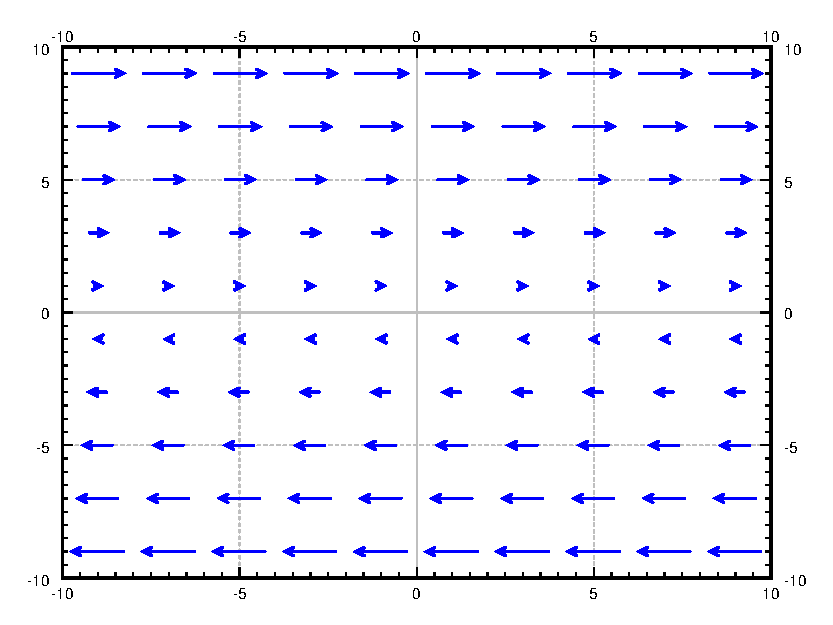
\includegraphics[width=2in]{figures/0100vectorfield}}}
%mbxENDIGNORE
%mbxlatex 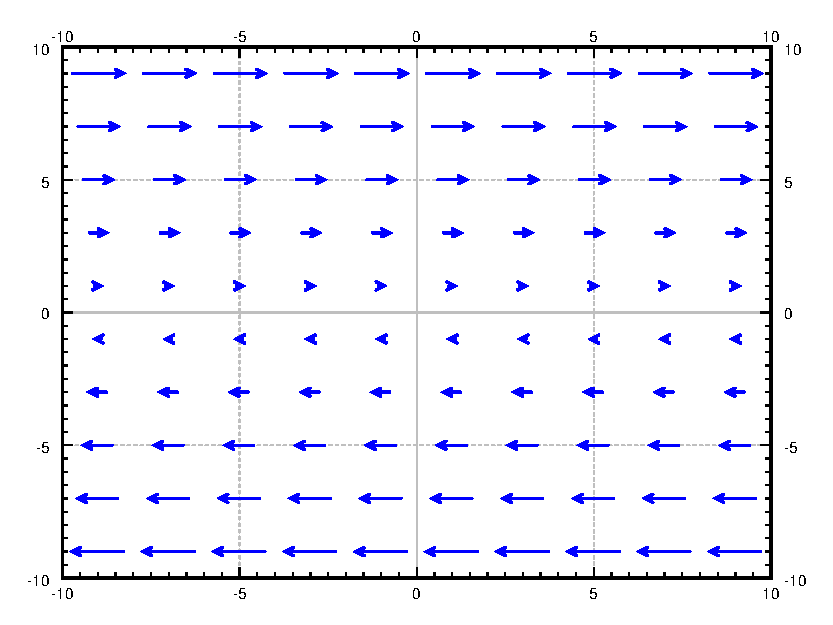
\includegraphics[width=2in]{figures/0100vectorfield}
\\[6pt]
The solution does not move anywhere if $y = 0$.  When $y$ is positive,
the solution moves (with constant speed)
in the positive $x$ direction.  When $y$ is
negative, the solution moves (with constant speed) in the negative
$x$ direction.  It is not one of the behaviors we saw.
\\
Note that the matrix has a double eigenvalue 0 and the general solution is
$x = C_1 t + C_2$ and $y = C_1$, which agrees with the
description above.
}

%%%%%%%%%%%%%%%%%%%%%%%%%%%%%%%%%%%%%%%%%%%%%%%%%%%%%%%%%%%%%%%%%%%%%%%%%%%%%%

\sectionnewpage
\section{Second order systems and applications}
\label{sol:section}

\sectionnotes{more than 2 lectures\EPref{, \S5.4 in \cite{EP}}\BDref{,
not in \cite{BD}}}

\subsection{Undamped mass-spring systems}

While we did say that we will usually only look at first order systems, it is
sometimes more convenient to study the system in the way it arises naturally.
For example, suppose we have 3 masses connected by springs between two
walls.  We could pick any higher number, and the math would be essentially
the same, but for simplicity we pick 3 right now.  Let us also assume no
friction, that is, the system is undamped\index{undamped motion!systems}.
The masses are $m_1$, $m_2$, and
$m_3$ and the spring constants are $k_1$, $k_2$, $k_3$, and $k_4$.
Let $x_1$ be the displacement from rest position of the first mass, and
$x_2$ and $x_3$ the displacement of the second and third mass.  We make,
as usual, positive values go right (as $x_1$ grows, the first mass is
moving right).
See \figurevref{sosa:threecartsfig}.

\begin{myfig}
\capstart
\inputpdft{threecartsfig}
\caption{System of masses and springs.\label{sosa:threecartsfig}}
\end{myfig}

This simple system turns up in unexpected places.  For example, 
our world really consists of many small particles of matter interacting together.
When we try the system above with many more masses, we obtain a good approximation to
how an elastic material behaves.  By somehow taking a limit of
the number of masses going to infinity, we obtain the continuous
one-dimensional wave equation (that we study in \sectionref{we:section}).
But we digress.

Let us set up the equations for the \myindex{three mass system}.
By \myindex{Hooke's law}, the force acting on the mass equals the 
spring compression times the spring constant.  By
\myindex{Newton's second law},
force is mass times acceleration.  So if we sum the forces acting
on each mass, put the right sign in front of each term, depending on the
direction in which it is acting, and set this equal to mass
times the acceleration, we end up with the desired system of
equations.
\begin{equation*}
\begin{aligned}
m_1 x_1'' &= -k_1 x_1 + k_2 (x_2-x_1)
& & = -(k_1+k_2) x_1 + k_2 x_2 , \\
m_2 x_2'' &= -k_2 (x_2-x_1) + k_3 (x_3-x_2)
& & = k_2 x_1 -(k_2+k_3) x_2 + k_3 x_3 , \\
m_3 x_3'' &= -k_3 (x_3-x_2) - k_4 x_3
& & = k_3 x_2 - (k_3+k_4) x_3 . 
\end{aligned}
\end{equation*}
We define the matrices
\begin{equation*}
M =
\begin{bmatrix}
m_1 & 0 & 0 \\
0 & m_2 & 0 \\
0 & 0 & m_3
\end{bmatrix}
\qquad
\text{and}
\qquad
K =
\begin{bmatrix}
-(k_1+k_2) & k_2 & 0 \\
k_2 & -(k_2+k_3) & k_3 \\
0 & k_3 & -(k_3+k_4)
\end{bmatrix} .
\end{equation*}
We write the equation simply as
\begin{equation*}
M {\vec{x}}'' = K \vec{x} .
\end{equation*}
At this point we could introduce 3 new variables and write out a system
of 6 first order equations.  We claim this simple setup is easier to handle as
a second order system.
We call $\vec{x}$ the \emph{\myindex{displacement vector}}, $M$ the
\emph{\myindex{mass matrix}}, and $K$ the \emph{\myindex{stiffness matrix}}.

\begin{exercise}
Repeat this setup for 4 masses (find the matrices $M$ and $K$).
Do it for 5 masses.  Can you
find a prescription to do it for $n$ masses?
\end{exercise}

As with a single equation we want to \myquote{divide by $M$.}  This means
computing the inverse of $M$.
The masses are all nonzero and $M$ is a
diagonal matrix\index{diagonal matrix}, so computing the inverse
is easy:
\begin{equation*}
M^{-1} =
\begin{bmatrix}
\frac{1}{m_1} & 0 & 0 \\
0 & \frac{1}{m_2} & 0 \\
0 & 0 & \frac{1}{m_3}
\end{bmatrix} .
\end{equation*}
This fact follows readily
by how we multiply diagonal matrices.  As an exercise, you should verify that
$M M^{-1} = M^{-1} M = I$.

\medskip

Let $A = M^{-1}K$.  We look at the system
${\vec{x}}'' = M^{-1}K \vec{x}$, or
\begin{equation*}
{\vec{x}}'' = A \vec{x} .
\end{equation*}
Many real world systems can be modeled by this equation.  For simplicity,
we will only talk about the
given masses-and-springs problem.  We try a solution of the form
\begin{equation*}
\vec{x} = \vec{v} e^{\alpha t} .
\end{equation*}
We compute that for this guess,
${\vec{x}}'' = \alpha^2 \vec{v} e^{\alpha t}$.
We plug our guess into the equation and get
\begin{equation*}
\alpha^2 \vec{v} e^{\alpha t} = A\vec{v} e^{\alpha t} .
\end{equation*}
We divide by $e^{\alpha t}$ to arrive at
$\alpha^2 \vec{v} = A\vec{v}$.  Hence if $\alpha^2$ is an eigenvalue
of $A$ and $\vec{v}$ is a corresponding eigenvector, we have found
a solution.

In our example, and in other common applications,
$A$ has only real negative
eigenvalues (and possibly a zero eigenvalue).  So we study only this
case.  When an eigenvalue $\lambda$ is negative, it means that
$\alpha^2 = \lambda$ is negative.  Hence there is some real number $\omega$
such that $-\omega^2 = \lambda$.  Then $\alpha = \pm i \omega$.
The solution we guessed was
\begin{equation*}
\vec{x} = \vec{v} \, \bigl(\cos (\omega t) + i \sin (\omega t) \bigr) .
\end{equation*}
By taking the real and imaginary parts (note that $\vec{v}$ is real), we
find that 
$\vec{v} \cos (\omega t)$ and
$\vec{v} \sin (\omega t)$ are linearly independent solutions.

If an eigenvalue is zero, it turns out that both $\vec{v}$ and $\vec{v} t$ are
solutions, where $\vec{v}$ is an eigenvector corresponding to the eigenvalue
0.

\begin{exercise}
Show that if $A$ has a zero eigenvalue and $\vec{v}$ is a
corresponding eigenvector, then $\vec{x} = \vec{v} (a + bt)$ is a solution
of ${\vec{x}}'' = A \vec{x}$ for
arbitrary constants $a$ and $b$.
\end{exercise}

\begin{theorem}
Let $A$ be a real $n \times n$ matrix
with $n$ distinct real negative (or zero) eigenvalues we
denote by $-\omega_1^2 > -\omega_2^2 > \cdots > -\omega_n^2$, and
corresponding
eigenvectors by
$\vec{v}_1$, $\vec{v}_2$, \ldots, $\vec{v}_n$.  If $A$ is invertible
(that is, if $\omega_1 > 0$), then
\begin{equation*}
\mybxbg{~~
\vec{x}(t)
= \sum_{i=1}^n \vec{v}_i \bigl(a_i \cos (\omega_i t) + b_i \sin (\omega_i t) \bigr) ,
~~}
\end{equation*}
is the general solution of
\begin{equation*}
{\vec{x}}'' = A \vec{x},
\end{equation*}
for some arbitrary constants $a_i$ and $b_i$.
If $A$ has a zero eigenvalue, that is $\omega_1 = 0$,
and all other eigenvalues are distinct and
negative, then the general solution can be written as
\begin{equation*}
\mybxbg{~~
\vec{x}(t) = \vec{v}_1 (a_1 + b_1 t) +
\sum_{i=2}^n \vec{v}_i \bigl(a_i \cos (\omega_i t) + b_i \sin (\omega_i t) \bigr) .
~~}
\end{equation*}
\end{theorem}

We use this solution and the setup from the introduction
of this section even when some of the masses and springs are missing.  
For example, when there are only 2 masses and only 2 springs, simply take
only the equations for
the two masses and set all the spring constants for the springs that
are missing to zero.

\subsection{Examples}

\begin{example}
Consider the setup in \figurevref{sosa:twocartswallfig}, with
$m_1 = \unit[2]{kg}$, $m_2 = \unit[1]{kg}$, $k_1 = \unitfrac[4]{N}{m}$, and
$k_2 = \unitfrac[2]{N}{m}$.

\begin{myfig}
\capstart
\inputpdft{twocartswallfig}
\caption{System of masses and springs.\label{sosa:twocartswallfig}}
\end{myfig}

The equations we write down are
\begin{equation*}
\begin{bmatrix}
2 & 0 \\
0 & 1
\end{bmatrix}
{\vec{x}}'' =
\begin{bmatrix}
-(4+2) & 2 \\
2 & -2
\end{bmatrix}
\vec{x} ,
\end{equation*}
or
\begin{equation*}
{\vec{x}}'' =
\begin{bmatrix}
-3 & 1 \\
2 & -2
\end{bmatrix}
\vec{x} .
\end{equation*}

We find the eigenvalues of $A$ to be $\lambda = -1, -4$ (exercise).
We find corresponding eigenvectors to be
$\left[ \begin{smallmatrix} 1 \\ 2 \end{smallmatrix} \right]$ and
$\left[ \begin{smallmatrix} 1 \\ -1 \end{smallmatrix} \right]$ respectively
(exercise).

We check the theorem and note that $\omega_1 = 1$ and $\omega_2 = 2$.
Hence the general solution is
\begin{equation*}
\vec{x} = 
\begin{bmatrix} 1 \\ 2 \end{bmatrix}
\bigl( a_1 \cos (t) + b_1 \sin (t) \bigr)
+
\begin{bmatrix} 1 \\ -1 \end{bmatrix}
\bigl( a_2 \cos (2t) + b_2 \sin (2t) \bigr) .
\end{equation*}

The two terms in the solution represent the two
so-called \emph{natural\index{natural mode of oscillation}}
or \emph{normal modes of oscillation\index{normal mode of oscillation}}.
And the two (angular) frequencies are the
\emph{natural frequencies\index{natural frequency}}.
The first natural frequency is 1, and second natural frequency is 2.
The two modes are plotted in \figurevref{sosa:modesfig}.

\begin{myfig}
\capstart
%original files sosa-mode1 sosa-mode2
\diffyincludegraphics{width=6.24in}{width=9in}{sosa-modes-1-2}
\caption{The two modes of the mass-spring system.  In the left plot
the masses are moving in unison and in the right plot are masses moving in the
opposite direction.\label{sosa:modesfig}}
\end{myfig}

Let us write the solution as
\begin{equation*}
\vec{x} = 
\begin{bmatrix} 1 \\ 2 \end{bmatrix}
c_1 \cos (t - \alpha_1 )
+
\begin{bmatrix} 1 \\ -1 \end{bmatrix}
c_2 \cos (2t - \alpha_2 ) .
\end{equation*}
The first term,
\begin{equation*}
\begin{bmatrix} 1 \\ 2 \end{bmatrix}
c_1 \cos (t - \alpha_1 )
=
\begin{bmatrix}
c_1 \cos (t - \alpha_1 ) \\
2c_1 \cos (t - \alpha_1 )
\end{bmatrix} ,
\end{equation*}
corresponds to the mode where the masses move synchronously
in the same direction.

The second term,
\begin{equation*}
\begin{bmatrix} 1 \\ -1 \end{bmatrix}
c_2 \cos (2t - \alpha_2 )
=
\begin{bmatrix}
c_2 \cos (2t - \alpha_2 ) \\
- c_2 \cos (2t - \alpha_2 )
\end{bmatrix} ,
\end{equation*}
corresponds to the mode where the masses move synchronously
but in opposite directions.

The general solution is a combination of the two modes.  That is, the
initial conditions determine the amplitude and phase shift of each mode.
As an example, suppose we have initial conditions
\begin{equation*}
\vec{x}(0) = 
\begin{bmatrix} 1 \\ -1 \end{bmatrix}
, \qquad
\vec{x}'(0) = 
\begin{bmatrix} 0 \\ 6 \end{bmatrix} .
\end{equation*}
We use the $a_j, b_j$ constants to solve for initial conditions.  First
\begin{equation*}
\begin{bmatrix} 1 \\ -1 \end{bmatrix}
=
\vec{x}(0) = 
\begin{bmatrix} 1 \\ 2 \end{bmatrix}
a_1
+
\begin{bmatrix} 1 \\ -1 \end{bmatrix}
a_2 
=
\begin{bmatrix} a_1+a_2 \\2a_1 - a_2 \end{bmatrix} .
\end{equation*}
We solve (exercise) to find $a_1 = 0$, $a_2 = 1$.
To find the $b_1$ and $b_2$, we differentiate first:
\begin{equation*}
{\vec{x}}' = 
\begin{bmatrix} 1 \\ 2 \end{bmatrix}
\bigl( - a_1 \sin (t) + b_1 \cos (t) \bigr)
+
\begin{bmatrix} 1 \\ -1 \end{bmatrix}
\bigl( - 2a_2 \sin (2t) + 2 b_2 \cos (2t) \bigr) .
\end{equation*}
Now we solve:
\begin{equation*}
\begin{bmatrix} 0 \\ 6 \end{bmatrix}
=
{\vec{x}}'(0) = 
\begin{bmatrix} 1 \\ 2 \end{bmatrix}
b_1
+
\begin{bmatrix} 1 \\ -1 \end{bmatrix}
2 b_2
=
\begin{bmatrix} b_1+2b_2 \\ 2b_1-2b_2 \end{bmatrix} .
\end{equation*}
Again solve (exercise) to find  $b_1 = 2$, $b_2 = -1$.  So our solution is
\begin{equation*}
\vec{x} = 
\begin{bmatrix} 1 \\ 2 \end{bmatrix}
2 \sin (t)
+
\begin{bmatrix} 1 \\ -1 \end{bmatrix}
\bigl( \cos (2t) - \sin (2t) \bigr)
=
\begin{bmatrix}
2 \sin (t) + \cos(2t)- \sin(2t) \\
4 \sin (t) - \cos(2t) + \sin(2t)
\end{bmatrix} .
\end{equation*}
The graphs of the two displacements, $x_1$ and $x_2$ of the two carts is in
\figurevref{sosa:superposfig}.
\begin{myfig}
\capstart
\diffyincludegraphics{width=3in}{width=4.5in}{sosa-superpos}
\caption{Superposition of the two modes given the initial
conditions.\label{sosa:superposfig}}
\end{myfig}
\end{example}

\begin{example} \label{sosa:railcarexample}
We have two toy rail
cars.  Car 1 of mass \unit[2]{kg} is traveling at \unitfrac[3]{m}{s}
towards the second
rail car of mass \unit[1]{kg}.  There is a bumper on the second rail car that
engages at the moment the cars hit (it connects to two cars)
and does not let go.
The bumper acts like a spring of spring constant $k=\unitfrac[2]{N}{m}$.
The second
car is 10 meters from a wall.  See \figurevref{sosa:railcarscrashfig}.

\begin{myfig}
\capstart
\inputpdft{railcarscrash}
\caption{The crash of two rail cars.\label{sosa:railcarscrashfig}}
\end{myfig}

We want to ask several questions.  At what time after the cars link does
impact with the wall happen?  What is the speed of car 2 when it hits the
wall?

OK\@, let us first set the system up.  Let $t=0$ be the time
when the two cars link up.  Let $x_1$ be the displacement of the first car
from the position at $t=0$, and let $x_2$ be the
displacement of the second car from its original location.  Then the
time when $x_2(t) = 10$ is exactly the time when impact with wall occurs.
For this $t$, $x_2'(t)$ is the speed at impact.  This system acts just like the
system of the previous example but without $k_1$.  Hence the equation is
\begin{equation*}
\begin{bmatrix}
2 & 0 \\
0 & 1
\end{bmatrix}
{\vec{x}}'' =
\begin{bmatrix}
-2 & 2 \\
2 & -2
\end{bmatrix}
\vec{x} ,
\end{equation*}
or
\begin{equation*}
{\vec{x}}'' =
\begin{bmatrix}
-1 & 1 \\
2 & -2
\end{bmatrix}
\vec{x} .
\end{equation*}

We compute the eigenvalues of $A$.  It is not hard to see that the eigenvalues
are 0 and $-3$ (exercise).  Furthermore,
eigenvectors are
$\left[ \begin{smallmatrix} 1 \\ 1 \end{smallmatrix} \right]$ and
$\left[ \begin{smallmatrix} 1 \\ -2 \end{smallmatrix} \right]$ respectively
(exercise). 
Then
$\omega_1 = 0$,
$\omega_2 = \sqrt{3}$, and by the second part of the theorem
the general solution is
\begin{equation*}
\begin{split}
\vec{x} & = 
\begin{bmatrix} 1 \\ 1 \end{bmatrix}
\left( a_1 + b_1 t \right) 
+
\begin{bmatrix} 1 \\ -2 \end{bmatrix}
\left( a_2 \cos ( \sqrt{3} \, t) + b_2 \sin ( \sqrt{3} \, t ) \right)
\\
& =
\begin{bmatrix}
a_1 + b_1 t + a_2 \cos ( \sqrt{3} \, t ) + b_2 \sin ( \sqrt{3} \, t
) \\
a_1 + b_1 t - 2 a_2 \cos ( \sqrt{3} \, t ) - 2 b_2 \sin ( \sqrt{3}
\, t ) 
\end{bmatrix} .
\end{split}
\end{equation*}

We now apply the initial conditions.  First the cars start at position 0
so $x_1 (0) = 0$ and $x_2(0) = 0$.  The first car is traveling at
\unitfrac[3]{m}{s},
so $x_1'(0) = 3$ and the second car starts at rest, so $x_2'(0) = 0$.
The first conditions says
\begin{equation*}
\vec{0} = \vec{x}(0) = 
\begin{bmatrix}
a_1 + a_2 \\
a_1 - 2 a_2 
\end{bmatrix} .
\end{equation*}
It is not hard to see that $a_1 = a_2 = 0$.  We set $a_1=0$
and $a_2=0$ in $\vec{x}(t)$
and differentiate to get
\begin{equation*}
{\vec{x}}'(t)
=
\begin{bmatrix}
b_1 + \sqrt{3} \, b_2 \cos ( \sqrt{3} \, t ) \\
b_1 - 2 \sqrt{3} \, b_2 \cos ( \sqrt{3} \, t )
\end{bmatrix} .
\end{equation*}
So
\begin{equation*}
\begin{bmatrix} 3 \\ 0 \end{bmatrix} = 
{\vec{x}}'(0)
=
\begin{bmatrix}
b_1 + \sqrt{3} \, b_2 \\
b_1 - 2 \sqrt{3} \, b_2 
\end{bmatrix} .
\end{equation*}
Solving these two equations we
find $b_1 = 2$ and $b_2 =
\frac{1}{\sqrt{3}}$.  Hence the position of our cars is
(until the impact with the wall)
\begin{equation*}
\vec{x} = 
\begin{bmatrix}
2 t + \frac{1}{\sqrt{3}} \sin ( \sqrt{3} \, t ) \\
2 t - \frac{2}{\sqrt{3}} \sin ( \sqrt{3} \, t )
\end{bmatrix} .
\end{equation*}
Note how the presence of the zero eigenvalue resulted in a term containing $t$.
This means that the cars will be traveling in the positive direction as
time grows, which is what we expect.


What we are really interested in is the second expression, the one for $x_2$.
We have $x_2(t) = 
2 t - \frac{2}{\sqrt{3}} \sin ( \sqrt{3} \, t)$.  See \figurevref{sosa:railcarfig}
for the plot of $x_2$ versus time.

Just from the graph we can see that time of impact will be a little
more than 5 seconds from time zero.  For this we have to solve
the equation $10 = x_2(t) = 2 t - \frac{2}{\sqrt{3}} \sin ( \sqrt{3} \,
t)$.
Using a computer (or even a graphing calculator)
we find that $t_{\text{impact}} \approx 5.22$ seconds.

\begin{mywrapfig}{3.25in}
\capstart
\diffyincludegraphics{width=3in}{width=4.5in}{sosa-railcar}
\caption{Position of the second car in time (ignoring the wall).\label{sosa:railcarfig}}
\end{mywrapfig}


The speed of the second car is $x_2' = 2 - 2 \cos ( \sqrt{3} \, t)$.
At the time of impact (5.22 seconds from $t=0$) we get 
$x_2'(t_{\text{impact}}) \approx 3.85$.
%
The maximum speed is the maximum of $2 - 2 \cos ( \sqrt{3} \, t )$, which is 4.
We are traveling at almost the maximum speed when we hit the wall.

\medskip

Suppose that Bob is a tiny person sitting on car 2.  Bob has a Martini in
his hand and would like not to spill it.  Let us suppose Bob would not spill
his Martini
when the first car links up with car 2, but if car 2 hits the wall at any
speed greater than zero, Bob will spill his drink.  Suppose Bob
can move car 2
a few meters towards or away from the wall (he cannot go all the way to the
wall, nor can he get out of the way of the first car).  Is there a
\myquote{safe}
distance for him to be at?  A distance such that the impact with
the wall is at zero speed?

The answer is yes.  On \figurevref{sosa:railcarfig},
note the \myquote{plateau} between $t=3$ and $t=4$.  There is a point where
the speed is zero.  To find it we solve $x_2'(t) = 0$.  This is when
$\cos ( \sqrt{3} \, t) = 1$ or in other words when $t = \frac{2 \pi}{\sqrt{3}}, 
\frac{4 \pi}{\sqrt{3}},\ldots$ and so on.  We plug in the first value to obtain
$x_2\left(\frac{2 \pi}{\sqrt{3}}\right) = 
\frac{4 \pi}{\sqrt{3}} \approx 7.26$.  So a \myquote{safe} distance is about 7 and a
quarter meters from the wall.

Alternatively Bob could move away from the wall
towards the incoming car 2, where another safe distance is
$x_2 \left( \frac{4 \pi}{\sqrt{3}} \right) = \frac{8 \pi}{\sqrt{3}}
\approx 14.51$ and so on.  We can use all the different
$t$ such that $x_2'(t) = 0$.  Of course $t=0$ is also a solution,
corresponding to $x_2 = 0$, but
that means standing right at the wall.
\end{example}

\subsection{Forced oscillations}

Finally we move to forced oscillations\index{forced motion!systems}.
Suppose that now our system is
\begin{equation} \label{sosa:forcedeq}
{\vec{x}}'' = A \vec{x} + \vec{F} \cos ( \omega t) .
\end{equation}
That is, we are adding periodic forcing to the system in the direction of
the vector $\vec{F}$.

As before, this system just requires us to find one particular solution
$\vec{x}_p$, add it to the general solution of the associated homogeneous system
$\vec{x}_c$, and we will have the general solution to \eqref{sosa:forcedeq}.
Let us suppose that $\omega$ is not one of the natural frequencies of
${\vec{x}}'' = A \vec{x}$, then we can guess
\begin{equation*}
\vec{x}_p = \vec{c} \cos (\omega t) ,
\end{equation*}
where $\vec{c}$ is an unknown constant vector.  Note that we do not need
to use sine since there are only second derivatives.  We solve for $\vec{c}$ to
find $\vec{x}_p$.  This is really just the method of
\emph{undetermined coefficients\index{undetermined coefficients!for second
order systems}}
for systems.  Let us differentiate $\vec{x}_p$ twice to get
\begin{equation*}
{\vec{x}_p}'' = -\omega^2 \vec{c} \cos (\omega t) .
\end{equation*}
Plug $\vec{x}_p$ and ${\vec{x}_p}''$ into equation \eqref{sosa:forcedeq}:
\begin{equation*}
\overbrace{
-\omega^2 \vec{c} \cos (\omega t)
}^{{\vec{x}_p}''}
=
\overbrace{
A \vec{c} \cos (\omega t) 
}^{A \vec{x}_p}
+ \vec{F} \cos (\omega t) .
\end{equation*}
We cancel out the cosine and rearrange the equation to obtain
\begin{equation*}
(A +\omega^2 I) \vec{c}
=
- \vec{F} .
\end{equation*}
So
\begin{equation*}
\vec{c}
=
{(A +\omega^2 I)}^{-1}
(-\vec{F} ).
\end{equation*}
Of course this is possible only if
$(A+ \omega^2 I) = \bigl(A- (-\omega^2) I\bigr)$ is
invertible.  That matrix is invertible if and only if
$-\omega^2$ is not an eigenvalue of $A$.  That is true if and only if $\omega$
is not a natural frequency of the system.

We simplified things a little bit.  If we wish to have the
forcing term to be in the units of force, say Newtons, then we must write
\begin{equation*}
M \vec{x}'' = K \vec{x} + \vec{G} \cos(\omega t) .
\end{equation*}
If we then write things in terms of $A = M^{-1} K$, we have
\begin{equation*}
\vec{x}'' = M^{-1}K \vec{x} + M^{-1} \vec{G} \cos(\omega t) 
\qquad \text{or} \qquad
\vec{x}'' = A \vec{x} + \vec{F} \cos(\omega t) ,
\end{equation*}
where $\vec{F} = M^{-1} \vec{G}$.

\begin{example}
Let us take the example in \figurevref{sosa:twocartswallfig} with
the same parameters as before:
$m_1 = 2$, $m_2 = 1$, $k_1 = 4$, and $k_2 = 2$.  Now suppose that
there is a force $2 \cos (3t)$ acting on the second cart.

The equation is
\begin{equation*}
\begin{bmatrix}
2 & 0 \\
0 & 1
\end{bmatrix}
{\vec{x}}'' =
\begin{bmatrix}
-(4+2) & 2 \\
2 & -2
\end{bmatrix}
\vec{x} 
+ 
\begin{bmatrix}
0 \\ 2
\end{bmatrix}
\cos (3 t) \qquad \text{or} \qquad
{\vec{x}}'' =
\begin{bmatrix}
-3 & 1 \\
2 & -2
\end{bmatrix}
\vec{x} 
+ 
\begin{bmatrix}
0 \\ 2
\end{bmatrix}
\cos (3 t) .
\end{equation*}
We solved the associated homogeneous equation before and found the
complementary solution to be
\begin{equation*}
\vec{x}_c =
\begin{bmatrix} 1 \\ 2 \end{bmatrix}
\bigl( a_1 \cos (t) + b_1 \sin (t) \bigr)
+
\begin{bmatrix} 1 \\ -1 \end{bmatrix}
\bigl( a_2 \cos (2t) + b_2 \sin (2t) \bigr) .
\end{equation*}

The natural frequencies are 1 and 2.  As 3 is not a
natural frequency, we try $\vec{c} \cos (3t)$.
We invert $(A+3^2 I)$:
\begin{equation*}
{\left( \begin{bmatrix}
-3 & 1 \\
\noalign{\smallskip}
2 & -2
\end{bmatrix}
+3^2 I\right)}^{-1}
=
{\begin{bmatrix}
6 & 1 \\
\noalign{\smallskip}
2 & 7
\end{bmatrix}}^{-1}
=
\begin{bmatrix}
\frac{7}{40} & \frac{-1}{40} \\
\noalign{\smallskip}
\frac{-1}{20} & \frac{3}{20}
\end{bmatrix} .
\end{equation*}
Hence,
\begin{equation*}
\vec{c} = 
{(A +\omega^2 I)}^{-1}
(-\vec{F} ) = 
\begin{bmatrix}
\frac{7}{40} & \frac{-1}{40} \\
\noalign{\smallskip}
\frac{-1}{20} & \frac{3}{20}
\end{bmatrix}
\begin{bmatrix}
0 \\
\noalign{\smallskip}
-2
\end{bmatrix}
=
\begin{bmatrix}
\frac{1}{20} \\
\noalign{\smallskip}
\frac{-3}{10}
\end{bmatrix} .
\end{equation*}

Combining with the general solution of the associated
homogeneous problem, we get that the general solution to
${\vec{x}}'' = A \vec{x} + \vec{F} \cos (\omega t)$ is
\begin{equation*}
\vec{x} = \vec{x}_c + \vec{x}_p =
\begin{bmatrix} 1 \\
\noalign{\smallskip}
2 \end{bmatrix}
\bigl( a_1 \cos (t) + b_1 \sin (t) \bigr)
+
\begin{bmatrix} 1 \\
\noalign{\smallskip}
-1 \end{bmatrix}
\bigl( a_2 \cos (2t) + b_2 \sin (2t) \bigr)
+
\begin{bmatrix}
\frac{1}{20} \\
\noalign{\smallskip}
\frac{-3}{10}
\end{bmatrix}
\cos (3t) .
\end{equation*}
We would then solve for the constants
$a_1$, $a_2$, $b_1$, and $b_2$ using
any given initial conditions.
\end{example}

Note that given force $\vec{f}$, we write 
the equation as $M {\vec{x}}'' = K \vec{x} + \vec{f}$ to get the units
right. Then we write
${\vec{x}}'' = M^{-1}K \vec{x} + M^{-1}\vec{f}$.  The 
term $\vec{g} = M^{-1} \vec{f}$ in ${\vec{x}}'' = A \vec{x} + \vec{g}$ is in units of force
per unit mass.

If $\omega$ is a natural frequency of the system,
\emph{\myindex{resonance}} may occur,
because we will have to try a particular solution of the form
\begin{equation*}
\vec{x}_p =
\vec{c} \, t \sin (\omega t) +
\vec{d} \, \cos (\omega t) .
\end{equation*}
That is assuming that the eigenvalues of the coefficient matrix are distinct.
Next, note that the amplitude of this solution grows without bound as $t$ grows.

\subsection{Exercises}

\begin{exercise}
Find a particular solution to
\begin{equation*}
{\vec{x}}'' =
\begin{bmatrix}
-3 & 1 \\
2 & -2
\end{bmatrix}
\vec{x} 
+ 
\begin{bmatrix}
0 \\ 2
\end{bmatrix}
\cos (2 t) .
\end{equation*}
\end{exercise}

\begin{exercise}[challenging]
Let us take the example in \figurevref{sosa:twocartswallfig} with
the same parameters as before:
$m_1 = 2$, $k_1 = 4$, and $k_2 = 2$, except for $m_2$, which is unknown.
Suppose that there is a force $\cos (5 t)$ acting on the first mass.
Find an $m_2$ such that there exists a particular solution where the
first mass does not move.

Note: This idea is called \emph{\myindex{dynamic damping}}.
In practice there will be a small amount of
damping and so any transient solution will disappear and after long enough
time, the first mass will always come to a stop.
\end{exercise}

\begin{exercise}
Let us take the \examplevref{sosa:railcarexample}, but that at
time of impact, car 2 is moving to the left at the speed of
\unitfrac[3]{m}{s}.
\begin{tasks}
\task
Find the behavior of the system after linkup.
\task
Will the second car hit
the wall, or will it be moving away from the wall as time goes on?
\task
At
what speed would the first car have to be traveling for the system to
essentially stay in place after linkup?
\end{tasks}
\end{exercise}

\begin{exercise}
Let us take the example in \figurevref{sosa:twocartswallfig} with
parameters
$m_1 = m_2 = 1$, $k_1 = k_2 = 1$.  Does there exist a set of initial
conditions for which the first cart moves but the second cart does not?
If so, find those conditions.  If not, argue why not.
\end{exercise}

\setcounter{exercise}{100}

\begin{exercise}
Find the general solution to
$\left[ \begin{smallmatrix}
1 & 0 & 0\\
0 & 2 & 0\\
0 & 0 & 3
\end{smallmatrix}\right]
\vec{x}\,''
=
\left[ \begin{smallmatrix}
-3 & 0 & 0 \\
2 & -4 & 0 \\
0 & 6 & -3
\end{smallmatrix}\right]
\vec{x}
+ 
\left[ \begin{smallmatrix}
\cos(2t) \\ 0 \\ 0
\end{smallmatrix}\right]$.
\end{exercise}
\exsol{%
$\vec{x}
=
\left[ \begin{smallmatrix}
1 \\ -1 \\ 1
\end{smallmatrix}\right]
\bigl( a_1 \cos (\sqrt{3}\, t)  + b_1 \sin (\sqrt{3}\, t) \bigr)
+
\left[ \begin{smallmatrix}
0 \\ 1 \\ -2
\end{smallmatrix}\right]
\bigl( a_2 \cos (\sqrt{2}\, t)  + b_2 \sin (\sqrt{2}\, t) \bigr)
+
$
\\
$
\left[ \begin{smallmatrix}
0 \\ 0 \\ 1
\end{smallmatrix}\right]
\bigl( a_3 \cos (t)  + b_3 \sin (t) \bigr)
+
\left[ \begin{smallmatrix}
-1 \\ \nicefrac{1}{2} \\ \nicefrac{2}{3}
\end{smallmatrix}\right]
\cos (2t)$
}

\begin{exercise}
Suppose there are three carts of equal mass $m$ and connected by two springs of
constant $k$ (and no connections to walls).  Set up the system and find its
general solution.
\end{exercise}
\exsol{%
$\left[ \begin{smallmatrix}
m & 0 & 0\\
0 & m & 0\\
0 & 0 & m
\end{smallmatrix}\right]
\vec{x}\,''
=
\left[ \begin{smallmatrix}
-k & k & 0 \\
k & -2k & k \\
0 & k & -k
\end{smallmatrix}\right]
\vec{x}$.
Solution:
$\vec{x} =
\left[ \begin{smallmatrix}
1 \\ -2 \\ 1
\end{smallmatrix}\right]
\bigl( a_1 \cos (\sqrt{\nicefrac{3k}{m}}\, t)  + b_1 \sin
(\sqrt{\nicefrac{3k}{m}}\, t) \bigr)
\allowbreak
+
\left[ \begin{smallmatrix}
1 \\ 0 \\ -1
\end{smallmatrix}\right]
\bigl( a_2 \cos (\sqrt{\nicefrac{k}{m}}\, t)  + b_2 \sin
(\sqrt{\nicefrac{k}{m}}\, t) \bigr)
+
\left[ \begin{smallmatrix}
1 \\ 1 \\ 1
\end{smallmatrix}\right]
\bigl( a_3 t  + b_3 \bigr).$
}

\begin{exercise}
Suppose a cart of mass \unit[2]{kg} is attached by a spring of
constant $k=1$ to a cart of mass \unit[3]{kg}, which
is attached to the wall by a spring also of constant $k=1$.
Suppose that the initial position of the first cart is 1 meter in the
positive direction from the rest position, and the second mass starts at the
rest position.  The masses are not moving and are let go.  Find the
position of the second mass as a function of time.
\end{exercise}
\exsol{%
$x_2 =
( \nicefrac{2}{5} )
\cos (\sqrt{\nicefrac{1}{6}}\, t)
-
( \nicefrac{2}{5} )
\cos (t)$
%sol
%$\vec{x} =
%\left[ \begin{smallmatrix}
%3 \\ 2
%\end{smallmatrix}\right]
%\bigl( a_1 \cos (\sqrt{\nicefrac{1}{6}}\, t)  + b_1 \sin
%(\sqrt{\nicefrac{1}{6}}\, t) \bigr)
%+
%\left[ \begin{smallmatrix}
%1 \\ -1
%\end{smallmatrix}\right]
%\bigl( a_2 \cos (t)  + b_2 \sin (t) \bigr)$.
}

%%%%%%%%%%%%%%%%%%%%%%%%%%%%%%%%%%%%%%%%%%%%%%%%%%%%%%%%%%%%%%%%%%%%%%%%%%%%%%

\sectionnewpage
\section{Multiple eigenvalues} \label{sec:multeigen}

\sectionnotes{1 or 1.5 lectures\EPref{, \S5.5 in \cite{EP}}\BDref{,
\S7.8 in \cite{BD}}}

It may happen that a matrix $A$ has some \myquote{repeated} eigenvalues.
That is, the characteristic equation $\det(A-\lambda I) = 0$ may have
repeated roots.  This is actually unlikely to happen
for a random matrix.  If we take a small perturbation of $A$ (we change the
entries of $A$ slightly), we get a matrix with distinct eigenvalues.  As
any system we want to solve in practice is an approximation to reality
anyway, it is not absolutely indispensable to know how to solve these
corner cases.  
On the other hand, these cases do come up in applications from time to time.
Furthermore, if we have distinct but very close eigenvalues, the behavior is
similar to that of repeated eigenvalues, and so understanding that case
will give us insight into what is going on.

\subsection{Geometric multiplicity}

Take the diagonal matrix
\begin{equation*}
A =
\begin{bmatrix}
3 & 0 \\ 0 & 3
\end{bmatrix} .
\end{equation*}
$A$ has an eigenvalue 3 of multiplicity 2.  We call the
multiplicity of the eigenvalue\index{multiplicity of an eigenvalue}
in the characteristic equation the
\emph{\myindex{algebraic multiplicity}}.  In this case, there also exist 2
linearly
independent eigenvectors,
$\left[ \begin{smallmatrix} 1 \\ 0 \end{smallmatrix} \right]$
and
$\left[ \begin{smallmatrix} 0 \\ 1 \end{smallmatrix} \right]$ corresponding
to the eigenvalue 3.  This means
that the so-called \emph{\myindex{geometric multiplicity}}
of this eigenvalue is also 2.

In all the
theorems where we required a matrix to have $n$ distinct eigenvalues, we only
really needed to have $n$ linearly independent eigenvectors.  For example,
${\vec{x}}' = A\vec{x}$ has the general solution
\begin{equation*}
\vec{x} = 
c_1 \begin{bmatrix} 1 \\ 0 \end{bmatrix} e^{3t}
+ c_2 \begin{bmatrix} 0 \\ 1 \end{bmatrix} e^{3t} .
\end{equation*}
Let us restate the theorem about real eigenvalues.  In the following theorem
we will repeat eigenvalues according to (algebraic) multiplicity.  So
for the matrix $A$ above, we would say that it has eigenvalues 3 and 3.

\begin{theorem}
Suppose the $n \times n$ matrix $P$ 
has $n$ real eigenvalues (not necessarily distinct), $\lambda_1$,
$\lambda_2$, \ldots, $\lambda_n$,
and there are $n$ linearly independent corresponding eigenvectors
$\vec{v}_1$, $\vec{v}_2$, \ldots, $\vec{v}_n$.  Then the general solution to 
${\vec{x}}' = P\vec{x}$
can be written as
\begin{equation*}
\vec{x} = c_1 \vec{v}_1 e^{\lambda_1 t} +
c_2 \vec{v}_2 e^{\lambda_2 t} + \cdots +
c_n \vec{v}_n e^{\lambda_n t} .
\end{equation*}
\end{theorem}

The \emph{geometric multiplicity} of an eigenvalue of algebraic multiplicity $n$
is equal to the number of corresponding linearly independent eigenvectors.
The geometric multiplicity is always less than or
equal to the algebraic multiplicity.  The theorem handles the case
when these two multiplicities are equal for all eigenvalues.
If for an eigenvalue the geometric multiplicity is equal
to the algebraic multiplicity, then we say the eigenvalue is
\emph{complete\index{complete eigenvalue}}.

In other words, 
the hypothesis of the theorem could be stated as saying that if all
the eigenvalues of $P$ are complete, then there are $n$ linearly independent
eigenvectors and thus we have the given general solution.

\medskip

If the geometric multiplicity of an eigenvalue is 2 or greater,
then the set of linearly independent eigenvectors is not unique up to
multiples as it was before.  For example, for the diagonal matrix $A =
\left[ \begin{smallmatrix} 3 & 0 \\ 0 & 3 \end{smallmatrix} \right]$
we could also pick eigenvectors
$\left[ \begin{smallmatrix} 1 \\ 1 \end{smallmatrix} \right]$
and
$\left[ \begin{smallmatrix} 1 \\ -1 \end{smallmatrix} \right]$, or in fact
any pair of two linearly independent vectors.  The number of linearly
independent eigenvectors corresponding to $\lambda$
is the number of free variables we obtain when solving $A\vec{v} =
\lambda \vec{v}$.  We pick specific values for those free variables to
obtain eigenvectors.  If you pick different values, you may get different
eigenvectors.


\subsection{Defective eigenvalues}

If an $n \times n$ matrix has less than $n$ linearly independent
eigenvectors, it is said to be \emph{deficient\index{deficient matrix}}.
Then there is at least
one eigenvalue with an algebraic multiplicity that is higher than its geometric
multiplicity.  We call this eigenvalue \emph{defective\index{defective
eigenvalue}}
and the difference
between the two multiplicities we call the \emph{\myindex{defect}}.

\begin{example}
The matrix
\begin{equation*}
\begin{bmatrix}
3 & 1 \\ 0 & 3
\end{bmatrix}
\end{equation*}
has an eigenvalue 3 of algebraic multiplicity 2.
Let us try to compute eigenvectors.
\begin{equation*}
\begin{bmatrix}
0 & 1 \\ 0 & 0
\end{bmatrix}
\begin{bmatrix}
v_1 \\ v_2
\end{bmatrix}
= \vec{0} .
\end{equation*}
We must have that $v_2 = 0$.  Hence any eigenvector is of the form
$\left[ \begin{smallmatrix} v_1 \\ 0 \end{smallmatrix} \right]$.  Any two
such vectors are linearly dependent, and hence the geometric multiplicity
of the eigenvalue is 1.  Therefore, the defect is 1, and we can no longer
apply the eigenvalue method directly to a system of ODEs with such a
coefficient matrix.

\medskip

Roughly, the key observation is that
if $\lambda$ is an eigenvalue of $A$ of algebraic multiplicity $m$,
then we can find certain $m$ linearly independent vectors
solving ${(A-\lambda I)}^k \vec{v} = \vec{0}$ for various powers
$k$.  We will call these \emph{\myindex{generalized eigenvectors}}.

\medskip

Let us continue with the example
$A = \left[ \begin{smallmatrix}
3 & 1 \\ 0 & 3
\end{smallmatrix} \right]$ and the equation ${\vec{x}}' = A\vec{x}$.
We found an eigenvalue $\lambda=3$ of (algebraic) multiplicity 2 and defect 1.
We found one eigenvector 
$\vec{v} = \left[ \begin{smallmatrix} 1 \\ 0 \end{smallmatrix} \right]$.
We have one solution
\begin{equation*}
\vec{x}_1 = \vec{v} e^{3t} = \begin{bmatrix} 1 \\ 0 \end{bmatrix} e^{3t} .
\end{equation*}
We are now stuck, we get no other solutions from standard eigenvectors.  But
we need two linearly independent solutions to find the general solution of
the equation.

Let us try (in the spirit of repeated roots of the
characteristic equation for a single equation) another solution of the form
\begin{equation*}
\vec{x}_2 = ( \vec{v}_2 +  \vec{v}_1 t )\, e^{3t} .
\end{equation*}
We differentiate to get
\begin{equation*}
{\vec{x}_2}' =
\vec{v}_1 e^{3t} +
3 ( \vec{v}_2 +  \vec{v}_1 t )\, e^{3t}
=
( 3 \vec{v}_2 + \vec{v}_1 )\, e^{3t} +  3 \vec{v}_1 t e^{3t} .
\end{equation*}
As we are assuming that $\vec{x}_2$ is a solution, ${\vec{x}_2}'$ must
equal $A \vec{x}_2$. So let's compute $A \vec{x}_2$:
\begin{equation*}
A \vec{x}_2 = 
A ( \vec{v}_2 +  \vec{v}_1 t )\, e^{3t}
=
A \vec{v}_2 e^{3t} +  A \vec{v}_1 t e^{3t} .
\end{equation*}
By looking at the coefficients of $e^{3t}$ and $t e^{3t}$ we see
$3 \vec{v}_2 + \vec{v}_1 = A \vec{v}_2$ and
$3 \vec{v}_1 = A \vec{v}_1$.
This means that
\begin{equation*}
(A-3I)\vec{v}_2 = \vec{v}_1,
\qquad \text{and} \qquad
(A-3I)\vec{v}_1 = \vec{0}.
\end{equation*}
Therefore, $\vec{x}_2$ is a solution
if these two equations are satisfied.
The second equation is satisfied if $\vec{v}_1$ is an
eigenvector, and we found the eigenvector above, so let
$\vec{v}_1 = 
\left[ \begin{smallmatrix} 1 \\ 0 \end{smallmatrix} \right]$.
So, if we can find a $\vec{v}_2$ that solves
%${(A-3I)}^2\vec{v}_2 = \vec{0}$ and such that
$(A-3I)\vec{v}_2 = \vec{v}_1$, then we are done.
This is just a bunch of linear
equations to solve and we are by now very good at that.
%
Let us solve
$(A-3I)\vec{v}_2 = \vec{v}_1$.  Write
\begin{equation*}
\begin{bmatrix}
0 & 1 \\ 0 & 0
\end{bmatrix}
\begin{bmatrix}
a \\ b
\end{bmatrix}
=
\begin{bmatrix}
1 \\ 0
\end{bmatrix} .
\end{equation*}
By inspection we see that letting $a=0$ ($a$ could be anything in fact) and
$b=1$ does the job.  Hence we can take $\vec{v}_2 = 
\left[ \begin{smallmatrix} 0 \\ 1 \end{smallmatrix} \right]$.  Our general
solution to
${\vec{x}}' = A\vec{x}$ is
\begin{equation*}
\vec{x} =
c_1 
\begin{bmatrix}
1 \\ 0
\end{bmatrix}
e^{3t}
+
c_2
\left(
\begin{bmatrix}
0 \\ 1
\end{bmatrix}
+
\begin{bmatrix}
1 \\ 0
\end{bmatrix}
t
\right)
\,
e^{3t}
=
\begin{bmatrix}
c_1 e^{3t}+c_2 te^{3t} \\
c_2 e^{3t}
\end{bmatrix} .
\end{equation*}
Let us check that we really do have the solution.  First
$x_1' = 
c_1 3 e^{3t}+c_2 e^{3t} + 3 c_2 te^{3t} = 3 x_1 + x_2$.  Good.  Now
$x_2' = 3 c_2 e^{3t} = 3x_2$.  Good.
\end{example}

In the example, if we plug $(A-3I)\vec{v}_2 = \vec{v}_1$ into
$(A-3I)\vec{v}_1 = \vec{0}$ we find
\begin{equation*}
(A-3I)(A-3I) \vec{v}_2 = \vec{0},
\qquad \text{or} \qquad
{(A-3I)}^2\vec{v}_2 = \vec{0}.
\end{equation*}
Furthermore, if 
$(A-3I) \vec{w} \not= \vec{0}$, then 
$(A-3I) \vec{w}$ is an eigenvector, a multiple of $\vec{v}_1$.
In this $2 \times 2$ case ${(A-3I)}^2$ is just the zero matrix (exercise).
So any vector $\vec{w}$ solves
${(A-3I)}^2\vec{w} = \vec{0}$ and we just need a $\vec{w}$ such that
$(A-3I)\vec{w} \not= \vec{0}$.  Then we could use
$\vec{w}$ for $\vec{v}_2$, and $(A-3I)\vec{w}$ for $\vec{v}_1$.

Note that the system ${\vec{x}}' = A \vec{x}$ has a simpler solution since
$A$ is a so-called \emph{\myindex{upper triangular matrix}}, that is
every entry below the diagonal is zero.
In particular, the equation for $x_2$
does not depend on $x_1$.  Mind you, not every defective matrix is
triangular.

\begin{exercise}
Solve ${\vec{x}}' = \left[ \begin{smallmatrix}
3 & 1 \\ 0 & 3
\end{smallmatrix} \right] \vec{x}$ by first solving for $x_2$ and then for
$x_1$ independently.  Check that you got the same solution as we did
above.
\end{exercise}

Let us describe the general algorithm.  Suppose that $\lambda$ is an
eigenvalue of multiplicity 2, defect 1.
First find an eigenvector $\vec{v}_1$ of $\lambda$.  
That is, $\vec{v}_1$ solves
$(A-\lambda I)\vec{v}_1  = \vec{0}$.
Then, find a vector $\vec{v}_2$ such that
\begin{equation*}
%{(A-\lambda I)}^2\vec{v}_2 & = \vec{0} , \\
(A-\lambda I)\vec{v}_2 = \vec{v}_1 .
\end{equation*}
This gives us two linearly independent solutions
\begin{align*}
\vec{x}_1 & = \vec{v}_1 e^{\lambda t} , \\
\vec{x}_2 & = \left( \vec{v}_2 + \vec{v}_1 t \right) e^{\lambda t} .
\end{align*}

\begin{example}
Consider the system
\begin{equation*}
\vec{x}' =
\begin{bmatrix}
2 & -5 & 0 \\
0 & 2 & 0 \\
-1 & 4 & 1
\end{bmatrix}
\vec{x} .
\end{equation*}
Compute the eigenvalues,
\begin{equation*}
0 =
\det(A-\lambda I) = 
\det\left(
\begin{bmatrix}
2-\lambda & -5 & 0 \\
0 & 2-\lambda & 0 \\
-1 & 4 & 1-\lambda
\end{bmatrix}
\right)
= (2-\lambda)^2(1-\lambda) .
\end{equation*}
The eigenvalues are 1 and 2, where 2 has multiplicity 2.
We leave it to the reader to find that
$\left[ \begin{smallmatrix} 0 \\ 0 \\ 1 \end{smallmatrix} \right]$
is an eigenvector
for the eigenvalue $\lambda = 1$.

Let's focus on $\lambda = 2$.  We compute eigenvectors:
\begin{equation*}
\vec{0} =
(A - 2 I) \vec{v}
=
\begin{bmatrix}
0 & -5 & 0 \\
0 & 0 & 0 \\
-1 & 4 & -1
\end{bmatrix}
\begin{bmatrix}
v_1 \\ v_2 \\ v_3
\end{bmatrix}
.
\end{equation*}
The first equation says that $v_2 = 0$, so the last equation
is $-v_1 -v_3 = 0$.  Let $v_3$ be the free variable to find
that $v_1 = -v_3$.  Perhaps let $v_3 = -1$ to find an eigenvector
$\left[ \begin{smallmatrix} 1 \\ 0 \\ -1 \end{smallmatrix} \right]$.
Problem is that setting $v_3$ to anything else just gets multiples
of this vector and so we have a defect of 1.
Let $\vec{v}_1$ be the eigenvector and let's look for
a generalized eigenvector $\vec{v}_2$:
\begin{equation*}
(A - 2 I) \vec{v}_2 = \vec{v}_1 , 
\end{equation*}
or
\begin{equation*}
\begin{bmatrix}
0 & -5 & 0 \\
0 & 0 & 0 \\
-1 & 4 & -1
\end{bmatrix}
\begin{bmatrix}
a \\ b \\ c
\end{bmatrix}
=
\begin{bmatrix}
1 \\ 0 \\ -1
\end{bmatrix} ,
\end{equation*}
where we used $a$, $b$, $c$ as components of $\vec{v}_2$ for simplicity.
The first equation says $-5b = 1$ so $b = \nicefrac{-1}{5}$.  The
second equation says nothing.
The last equation is $-a + 4b - c = -1$, or
$a + \nicefrac{4}{5} + c = 1$, or
$a + c = \nicefrac{1}{5}$.  We let $c$ be the free variable and we
choose $c=0$.  We find
$\vec{v}_2 = \left[ \begin{smallmatrix} \nicefrac{1}{5} \\ \nicefrac{-1}{5}
\\ 0 \end{smallmatrix} \right]$.

The general solution is therefore,
\begin{equation*}
\vec{x} =
c_1
\begin{bmatrix} 0 \\ 0 \\ 1 \end{bmatrix}
e^t
+
c_2 
\begin{bmatrix} 1 \\ 0 \\ -1 \end{bmatrix}
e^{2t}
+
c_3
\left(
\begin{bmatrix} \nicefrac{1}{5} \\ \nicefrac{-1}{5} \\ 0 \end{bmatrix}
+
\begin{bmatrix} 1 \\ 0 \\ -1 \end{bmatrix}
t
\right)
e^{2t}
.
\end{equation*}
\end{example}

This machinery can also be generalized to higher multiplicities
and higher defects.
We will not go over this method in detail, but let us just sketch the ideas.  Suppose that $A$
has an eigenvalue $\lambda$ of multiplicity $m$.
We find vectors such that
\begin{equation*}
{(A - \lambda I)}^k \vec{v} = \vec{0},
\qquad \text{but} \qquad
{(A - \lambda I)}^{k-1} \vec{v} \not= \vec{0}.
\end{equation*}
Such vectors are called \emph{\myindex{generalized eigenvectors}} (then
$\vec{v}_1 = {(A - \lambda I)}^{k-1} \vec{v}$ is an eigenvector).
For the
eigenvector $\vec{v}_1$ there is a chain of generalized eigenvectors
$\vec{v}_2$ through $\vec{v}_k$ such that:
\begin{align*}
(A - \lambda I) \vec{v}_1 & = \vec{0} , \\
(A - \lambda I) \vec{v}_2 & = \vec{v}_1 , \\
& ~~\vdots \\
(A - \lambda I) \vec{v}_k & = \vec{v}_{k-1} .
\end{align*}
Really once you find the $\vec{v}_k$ such that
${(A - \lambda I)}^k \vec{v}_k = \vec{0}$ but
${(A - \lambda I)}^{k-1} \vec{v}_k \not= \vec{0}$, you find the entire
chain since you can compute the rest,
$\vec{v}_{k-1} = (A - \lambda I) \vec{v}_k$,
$\vec{v}_{k-2} = (A - \lambda I) \vec{v}_{k-1}$, etc.
We form the linearly independent solutions
\begin{align*}
\vec{x}_1 & = \vec{v}_1 e^{\lambda t} , \\
\vec{x}_2 & = ( \vec{v}_2 + \vec{v}_1 t ) \, e^{\lambda t} , \\
& ~~\vdots \\
\vec{x}_k & = \left( \vec{v}_k + \vec{v}_{k-1} t +
\vec{v}_{k-2} \frac{t^2}{2} +
\cdots + \vec{v}_2 \frac{t^{k-2}}{(k-2)!} + \vec{v}_1 \frac{t^{k-1}}{(k-1)!}
\right) \, e^{\lambda t} .
\end{align*}
Recall that $k! = 1 \cdot 2 \cdot 3 \cdots (k-1) \cdot k$ is the factorial.
If you have an eigenvalue of geometric multiplicity $\ell$,
you will have to find $\ell$ such chains (some of them might be
short: just the single eigenvector equation).
We go until we form $m$ linearly independent solutions where
$m$ is the algebraic multiplicity.
We don't quite know which specific eigenvectors go with which chain, so
start by finding $\vec{v}_k$ first for the longest possible chain and
go from there.

For example, if $\lambda$ is an eigenvalue of $A$
of algebraic multiplicity 3 and defect 2, then solve
\begin{equation*}
(A - \lambda I) \vec{v}_1 = \vec{0} , \qquad
(A - \lambda I) \vec{v}_2 = \vec{v}_1 , \qquad
(A - \lambda I) \vec{v}_3 = \vec{v}_2 .
\end{equation*}
That is, find $\vec{v}_3$ such that 
${(A - \lambda I)}^3 \vec{v}_3 = \vec{0}$, but
${(A - \lambda I)}^2 \vec{v}_3 \not= \vec{0}$.
Then you are done as
$\vec{v}_2 = (A - \lambda I) \vec{v}_3$
and 
$\vec{v}_1 = (A - \lambda I) \vec{v}_2$.
The 3 linearly independent solutions are
\begin{equation*}
\vec{x}_1 = \vec{v}_1 e^{\lambda t} , \qquad
\vec{x}_2 = ( \vec{v}_2 + \vec{v}_1 t ) \, e^{\lambda t} , \qquad
\vec{x}_3 = \left( \vec{v}_3 + \vec{v}_2 t +
\vec{v}_{1} \frac{t^2}{2} \right) \, e^{\lambda t} .
\end{equation*}

If, on the other hand, $A$ has an eigenvalue $\lambda$
of algebraic multiplicity 3 and defect 1, then 
solve
\begin{equation*}
(A - \lambda I) \vec{v}_1 = \vec{0} , \qquad
(A - \lambda I) \vec{v}_2 = \vec{0} , \qquad
(A - \lambda I) \vec{v}_3 = \vec{v}_2 .
\end{equation*}
Here $\vec{v}_1$ and $\vec{v}_2$ are actual honest eigenvectors,
and $\vec{v}_3$ is a generalized eigenvector.
So there are two chains.
To solve, first find a 
$\vec{v}_3$ such that 
${(A - \lambda I)}^2 \vec{v}_3 = \vec{0}$, but
$(A - \lambda I) \vec{v}_3 \not= \vec{0}$.
Then $\vec{v}_2 = (A - \lambda I) \vec{v}_3$ is going to be an eigenvector.
Then solve for an eigenvector $\vec{v}_1$ that is linearly independent 
from $\vec{v}_2$.
You get 3 linearly independent solutions
\begin{equation*}
\vec{x}_1 = \vec{v}_1 e^{\lambda t} , \qquad
\vec{x}_2 = \vec{v}_2 e^{\lambda t} , \qquad
\vec{x}_3 = ( \vec{v}_3 + \vec{v}_2 t ) \, e^{\lambda t} .
\end{equation*}

\subsection{Exercises}

\begin{exercise}
Let
$A = \left[ \begin{smallmatrix} 5 & -3 \\ 3 & -1 \end{smallmatrix} \right]$.
Find the general solution of ${\vec{x}}' = A \vec{x}$.
\end{exercise}

\begin{samepage}
\begin{exercise}
Let
$A = \left[ \begin{smallmatrix}
5 & -4 & 4 \\
0 & 3 & 0 \\
-2 & 4 & -1
\end{smallmatrix} \right]$.
\begin{tasks}
\task What are the eigenvalues?
\task What is/are the defect(s) of the eigenvalue(s)?
\task Find the general solution of ${\vec{x}}' = A \vec{x}$.
\end{tasks}
\end{exercise}
\end{samepage}


\begin{exercise}
Let
$A = \left[ \begin{smallmatrix} 2 & 1 & 0 \\ 0 & 2 & 0 \\ 0 & 0 & 2 \end{smallmatrix} \right]$.
\begin{tasks}
\task What are the eigenvalues?
\task What is/are the defect(s) of the eigenvalue(s)?
\task Find the general solution of ${\vec{x}}' = A \vec{x}$ in two different
ways and verify you get the same answer.
\end{tasks}
\end{exercise}

\begin{exercise}
Let
$A = \left[ \begin{smallmatrix}
0 & 1 & 2 \\
-1 & -2 & -2 \\
-4 & 4 & 7
\end{smallmatrix} \right]$.
\begin{tasks}
\task What are the eigenvalues?
\task What is/are the defect(s) of the eigenvalue(s)?
\task Find the general solution of ${\vec{x}}' = A \vec{x}$.
\end{tasks}
\end{exercise}

\begin{exercise}
\pagebreak[2]
Let
$A = \left[ \begin{smallmatrix}
0 & 4 & -2 \\
-1 & -4 & 1 \\
0 & 0 & -2
\end{smallmatrix} \right]$.
\begin{tasks}
\task What are the eigenvalues?
\task What is/are the defect(s) of the eigenvalue(s)?
\task Find the general solution of ${\vec{x}}' = A \vec{x}$.
\end{tasks}
\end{exercise}

\begin{exercise}
Let
$A = \left[ \begin{smallmatrix}
2 & 1 & -1 \\
-1 & 0 & 2 \\
-1 & -2 & 4
\end{smallmatrix} \right]$.
\begin{tasks}
\task What are the eigenvalues?
\task What is/are the defect(s) of the eigenvalue(s)?
\task Find the general solution of ${\vec{x}}' = A \vec{x}$.
\end{tasks}
\end{exercise}

\begin{exercise}
Suppose that $A$ is a $2 \times 2$ matrix with a repeated eigenvalue
$\lambda$.
Suppose that there are two linearly independent eigenvectors.  Show that
$A = \lambda I$.
\end{exercise}

\setcounter{exercise}{100}

\begin{exercise}
Let $A =
\left[ \begin{smallmatrix}
1 & 1 & 1 \\
1 & 1 & 1 \\
1 & 1 & 1 
\end{smallmatrix}\right]$.  
\begin{tasks}
\task What are the eigenvalues?
\task What is/are the defect(s) of the eigenvalue(s)?
\task Find the general solution of $\vec{x}\,' = A\vec{x}$.
\end{tasks}
\end{exercise}
\exsol{%
a) $3,0,0$
\quad
b) No defects.
\quad
c)
$\vec{x} =
C_1
\left[ \begin{smallmatrix}
1 \\ 1 \\ 1
\end{smallmatrix}\right]
e^{3t}
+
C_2
\left[ \begin{smallmatrix}
1 \\ 0 \\ -1
\end{smallmatrix}\right]
+
C_3
\left[ \begin{smallmatrix}
0 \\ 1 \\ -1
\end{smallmatrix}\right]$
}

\begin{exercise}
Let $A =
\left[ \begin{smallmatrix}
1 & 3 & 3 \\
1 & 1 & 0 \\
-1 & 1 & 2 \\
\end{smallmatrix}\right]$.  
\begin{tasks}
\task What are the eigenvalues?
\task What is/are the defect(s) of the eigenvalue(s)?
\task Find the general solution of $\vec{x}\,' = A\vec{x}$.
\end{tasks}
\end{exercise}
\exsol{%
a) $1,1,2$
\\
b) Eigenvalue 1 has a defect of 1
\\
c)
$\vec{x} =
C_1
\left[ \begin{smallmatrix}
0 \\ 1 \\ -1
\end{smallmatrix}\right]
e^{t}
+
C_2
\left(
\left[ \begin{smallmatrix}
1 \\ 0 \\ 0
\end{smallmatrix}\right]
+
t
\left[ \begin{smallmatrix}
0 \\ 1 \\ -1
\end{smallmatrix}\right]
\right)
e^{t}
+
C_3
\left[ \begin{smallmatrix}
3 \\ 3 \\ -2
\end{smallmatrix}\right]
e^{2t}$
}

\begin{exercise}
Let $A =
\left[ \begin{smallmatrix}
2 & 0 & 0 \\
-1 & -1 & 9 \\
0 & -1 & 5
\end{smallmatrix}\right]$.  
\begin{tasks}
\task What are the eigenvalues?
\task What is/are the defect(s) of the eigenvalue(s)?
\task Find the general solution of $\vec{x}\,' = A\vec{x}$.
\end{tasks}
\end{exercise}
\exsol{%
a) $2,2,2$
\\
b) Eigenvalue 2 has a defect of 2
\\
c)
$\vec{x} =
C_1
\left[ \begin{smallmatrix}
0 \\ 3 \\ 1
\end{smallmatrix}\right]
e^{2t}
+
C_2
\left(
\left[ \begin{smallmatrix}
0 \\ -1 \\ 0
\end{smallmatrix}\right]
+
t
\left[ \begin{smallmatrix}
0 \\ 3 \\ 1
\end{smallmatrix}\right]
\right)
e^{2t}
+
C_3
\left(
\left[ \begin{smallmatrix}
1 \\ 0 \\ 0
\end{smallmatrix}\right]
+
t
\left[ \begin{smallmatrix}
0 \\ -1 \\ 0
\end{smallmatrix}\right]
+
\frac{t^2}{2}
\left[ \begin{smallmatrix}
0 \\ 3 \\ 1
\end{smallmatrix}\right]
\right)
e^{2t}$
}

\begin{exercise}
Let $A =
\left[ \begin{smallmatrix}
a & a \\
b & c
\end{smallmatrix}\right]$, where $a$, $b$, and $c$ are unknowns.
Suppose that $5$ is a doubled eigenvalue of defect 1, and suppose that
$\left[ \begin{smallmatrix}
1 \\ 0
\end{smallmatrix}\right]$ is a corresponding eigenvector.  Find $A$ and show that
there is only one such matrix $A$.
\end{exercise}
\exsol{%
$A = \left[ \begin{smallmatrix}
5 & 5 \\ 0 & 5
\end{smallmatrix}\right]$
}

%%%%%%%%%%%%%%%%%%%%%%%%%%%%%%%%%%%%%%%%%%%%%%%%%%%%%%%%%%%%%%%%%%%%%%%%%%%%%%

\sectionnewpage
\section{Matrix exponentials} \label{sec:matexp}

\sectionnotes{2 lectures\EPref{, \S5.6 in \cite{EP}}\BDref{,
\S7.7 in \cite{BD}}}

\subsection{Definition}

There is another way of finding a fundamental
matrix solution of a system.  Consider the constant
coefficient equation
\begin{equation*}
{\vec{x}}' = P \vec{x} .
\end{equation*}
If this would be just one equation (when $P$ is a number or a $1
\times 1$ matrix), then the solution would be
\begin{equation*}
\vec{x} = e^{Pt} .
\end{equation*}
That doesn't make sense if $P$ is a larger matrix, but
essentially the same computation that led to the above
works for matrices when we define
$e^{Pt}$ properly.  First let us write down the Taylor series for $e^{at}$
for some number $a$:
\begin{equation*}
e^{at} = 1 + at
+ \frac{{(at)}^2}{2}
+ \frac{{(at)}^3}{6}
+ \frac{{(at)}^4}{24}
+ \cdots
= \sum_{k=0}^\infty \frac{{(at)}^k}{k!} .
\end{equation*}
Recall $k! = 1 \cdot 2 \cdot 3 \cdots k$ is the factorial, and $0! = 1$.
We differentiate this series term by term
\begin{equation*}
\frac{d}{dt} \left(e^{at} \right) = 
0
+ a
+ a^2 t
+ \frac{a^3t^2}{2}
+ \frac{a^4t^3}{6}
+ \cdots
= a \left(
1
+ a t
+ \frac{{(at)}^2}{2}
+ \frac{{(at)}^3}{6}
+ \cdots \right)
= a e^{at}.
\end{equation*}
Maybe we can try the same trick with matrices.  For an $n \times n$
matrix $A$ we define the
\emph{\myindex{matrix exponential}\index{exponential of a matrix}} as
\begin{equation*}
\mybxbg{~~
e^A \overset{\text{def}}{=} I + A + \frac{1}{2} A^2 + 
\frac{1}{6} A^3 + \cdots + \frac{1}{k!} A^k + \cdots
~~}
\end{equation*}
Let us not worry about convergence.  The series really does
always converge.
We usually write $Pt$ as $tP$ by convention when $P$ is a matrix.
With this small change and by the exact same
calculation as above
we have that
\begin{equation*}
\frac{d}{dt} \left(e^{tP} \right) = 
P e^{tP} .
\end{equation*}
Now $P$ and hence $e^{tP}$ is an $n \times n$ matrix.  What we are looking
for is a vector.  In the $1 \times 1$ case we would at this
point multiply by an arbitrary constant to get the general solution.  In the
matrix case we multiply by a column vector $\vec{c}$.

\begin{theorem}
Let $P$ be an $n \times n$ matrix.  Then the general solution to
${\vec{x}}' = P \vec{x}$ is
\begin{equation*}
\vec{x} = e^{tP} \vec{c} ,
\end{equation*}
where $\vec{c}$ is an arbitrary constant vector.  In fact, $\vec{x}(0) =
\vec{c}$.
\end{theorem}

Let us check:
\begin{equation*}
\frac{d}{dt}
\vec{x} =
\frac{d}{dt} \left( 
e^{tP} \vec{c}\, \right)
=
P e^{tP} \vec{c} =
P \vec{x}.
\end{equation*}

Hence $e^{tP}$ is a \myindex{fundamental matrix solution}
of the homogeneous system.
So if we can compute the matrix exponential,
we have another method of solving constant coefficient homogeneous
systems.  It also makes it easy to solve for initial conditions.  To solve 
${\vec{x}}' = A \vec{x}$, $\vec{x}(0) = \vec{b}$, we take the solution
\begin{equation*}
\vec{x} = e^{tA} \vec{b} .
\end{equation*}
This equation follows because $e^{0A} = I$,
so $\vec{x} (0) = e^{0A} \vec{b} = \vec{b}$.

\medskip

We mention a drawback of matrix exponentials.
In general $e^{A+B} \not= e^A e^B$.  The trouble is that matrices do
not commute, that is, in general $AB \not= BA$.
If you try to prove $e^{A+B} \not= e^A e^B$ using the Taylor series,
you will see why the lack of commutativity becomes a problem.
However, it is still true that if
$AB = BA$, that is, if $A$ and $B$ commute, then $e^{A+B} = e^Ae^B$.  We will
find this fact useful.  Let us restate this as a theorem to make a point.

\begin{theorem}
If $AB = BA$, then $e^{A+B} = e^Ae^B$.  Otherwise,
$e^{A+B} \not= e^Ae^B$ in general.
\end{theorem}

\subsection{Simple cases}

In some instances it may work to just plug into the series definition.
Suppose the matrix is diagonal\index{diagonal matrix!matrix exponential of}.
For example,
$D = \left[ \begin{smallmatrix} a & 0 \\ 0 & b \end{smallmatrix} \right]$.
Then 
\begin{equation*}
D^k = \begin{bmatrix} a^k & 0 \\ 0 & b^k \end{bmatrix} ,
\end{equation*}
and
\begin{equation*}
\begin{split}
e^D & =
I + D + \frac{1}{2} D^2 + 
\frac{1}{6} D^3 + \cdots
\\
&=
\begin{bmatrix} 1 & 0 \\ 0 & 1 \end{bmatrix} +
\begin{bmatrix} a & 0 \\ 0 & b \end{bmatrix} +
\frac{1}{2}
\begin{bmatrix} a^2 & 0 \\ 0 & b^2 \end{bmatrix} +
\frac{1}{6}
\begin{bmatrix} a^3 & 0 \\ 0 & b^3 \end{bmatrix} + \cdots
=
\begin{bmatrix} e^a & 0 \\ 0 & e^b \end{bmatrix} .
\end{split}
\end{equation*}
So by this rationale
\begin{equation*}
e^I = \begin{bmatrix} e & 0\\ 0 & e \end{bmatrix}
\qquad \text{and} \qquad
e^{aI} = \begin{bmatrix} e^a & 0\\ 0 & e^a \end{bmatrix}.
\end{equation*}

This makes exponentials of certain other matrices easy to compute.  
For example, the matrix
$A = \left[ \begin{smallmatrix} 5 & 4 \\ -1 & 1 \end{smallmatrix} \right]$
can be written as
$3I + B$ where
$B = \left[ \begin{smallmatrix} 2 & 4 \\ -1 & -2 \end{smallmatrix} \right]$.
Notice that $B^2 = 
\left[ \begin{smallmatrix} 0 & 0 \\ 0 & 0 \end{smallmatrix} \right]$.  So
$B^k = 0$ for all $k \geq 2$.  Therefore, $e^B = I + B$.  Suppose we
actually want to compute $e^{tA}$.  The matrices $3tI$ and $tB$ commute
(exercise: check this)
and $e^{tB} = I + tB$, since ${(tB)}^2 = t^2 B^2 = 0$.
We write
\begin{multline*}
e^{tA} = 
e^{3tI + tB} = e^{3tI} e^{tB} = 
\begin{bmatrix} e^{3t} & 0 \\ 0 & e^{3t} \end{bmatrix}
\left(
I + tB
\right)
=
\\
=
\begin{bmatrix} e^{3t} & 0 \\ 0 & e^{3t} \end{bmatrix}
\begin{bmatrix} 1+2t & 4t \\ -t & 1-2t \end{bmatrix}
=
\begin{bmatrix} (1+2t)\,e^{3t} & 4te^{3t} \\ -te^{3t} & (1-2t)\,e^{3t} \end{bmatrix} .
\end{multline*}
We found a fundamental matrix solution for the
system ${\vec{x}}' = A \vec{x}$.  Note that this matrix has a repeated
eigenvalue with a defect; there is only one eigenvector for the eigenvalue
3.  So we found a perhaps easier way to handle this case.  In fact, if
a matrix $A$ is $2 \times 2$ and has an eigenvalue $\lambda$ of multiplicity
2, then
either $A = \lambda I$, or $A = \lambda I + B$ where $B^2 = 0$.  This is a
good exercise.

\begin{exercise}%[challenging] No longer challenging with the hint?
Suppose that $A$ is $2 \times 2$ and $\lambda$
is the only eigenvalue.  Show that ${(A - \lambda I)}^2 = 0$, and therefore
that we can write $A = \lambda I + B$, where $B^2 = 0$ (and possibly $B=0$).
Hint: First
write down what does it mean for the eigenvalue to be of multiplicity 2.
You will get
an equation for the entries.  Now compute the square of $B$.
\end{exercise}

Matrices $B$ such that $B^k = 0$ for some $k$ are called
\emph{\myindex{nilpotent}}.  Computation of the matrix exponential for
nilpotent matrices is easy by just writing down the first $k$ terms of
the Taylor series.

\subsection{General matrices}

In general, the exponential is not as easy to compute as above.  We usually
cannot write a matrix as a sum of commuting matrices where the exponential
is simple for each one.  But fear not, it is still not too difficult provided
we can find enough eigenvectors.  First we need the following interesting
result about matrix exponentials.  For two square matrices $A$ and $B$, with
$B$ invertible,
we have
\begin{equation*}
e^{BAB^{-1}} = B e^A B^{-1} .
\end{equation*}
This can be seen by writing down the Taylor series.  First 
\begin{equation*}
{(BAB^{-1})}^2 =
BAB^{-1} BAB^{-1} =
BAIAB^{-1} =
BA^2B^{-1} .
\end{equation*}
And by the same reasoning ${(BAB^{-1})}^k = B A^k B^{-1}$.  Now write 
the Taylor series for
$e^{BAB^{-1}}$:
\begin{equation*}
\begin{split}
e^{BAB^{-1}} & =
I + {BAB^{-1}} + \frac{1}{2} {(BAB^{-1})}^2 + 
\frac{1}{6} {(BAB^{-1})}^3 + \cdots
\\
& =
BB^{-1} + {BAB^{-1}} + \frac{1}{2} BA^2B^{-1} + 
\frac{1}{6} BA^3B^{-1} + \cdots
\\
& =
B \bigl(
I + A + \frac{1}{2} A^2 + 
\frac{1}{6} A^3 + \cdots \bigr) B^{-1} \\
& = B e^A B^{-1} .
\end{split}
\end{equation*}

Given a square matrix $A$, 
we can usually write $A = E D E^{-1}$, where $D$ is
diagonal and $E$ invertible.
This procedure is called \emph{\myindex{diagonalization}}.
If we can do
that, the computation  of the
exponential becomes easy as $e^D$ is just taking the exponential of
the entries on the diagonal.  Adding $t$ into the mix, 
we can then compute the exponential
\begin{equation*}
e^{tA} = E e^{tD} E^{-1} .
\end{equation*}

To diagonalize $A$
we need $n$ linearly independent eigenvectors of $A$.
Otherwise, this method of computing the exponential does not work and we need to be trickier, but we will
not get into such details.
Let $E$ be the matrix with the eigenvectors as columns.  
Let $\lambda_1$, $\lambda_2$, \ldots, $\lambda_n$ be the eigenvalues and
let $\vec{v}_1$, $\vec{v}_2$, \ldots, $\vec{v}_n$ be the eigenvectors, then
$E = [\, \vec{v}_1 \quad \vec{v}_2 \quad \cdots \quad \vec{v}_n \,]$.
Make a diagonal matrix $D$ with the eigenvalues on the diagonal:
\begin{equation*}
D =
\begin{bmatrix}
\lambda_1 & 0 & \cdots & 0 \\
0 & \lambda_2 & \cdots & 0 \\
\vdots & \vdots & \ddots & \vdots \\
0 & 0 & \cdots & \lambda_n
\end{bmatrix} .
\end{equation*}
We compute
\begin{equation*}
\begin{split}
AE & = A 
[\, \vec{v}_1 \quad \vec{v}_2 \quad \cdots \quad \vec{v}_n \,]
\\
& =
[\, A\vec{v}_1 \quad A\vec{v}_2 \quad \cdots \quad A\vec{v}_n \,]
\\
& =
[\, \lambda_1 \vec{v}_1 \quad \lambda_2 \vec{v}_2 \quad \cdots \quad
\lambda_n \vec{v}_n \,]
\\
& =
[\, \vec{v}_1 \quad \vec{v}_2 \quad \cdots \quad \vec{v}_n \,] D
\\
& =
ED .
\end{split}
\end{equation*}
The columns of $E$ are linearly independent as these are
linearly independent eigenvectors of
$A$.  Hence $E$ is invertible.
Since $AE = ED$, we multiply on the right by $E^{-1}$ and we get
\begin{equation*}
A = E D E^{-1}.
\end{equation*}
This means that $e^A = E e^D E^{-1}$.  Multiplying the matrix by $t$ we obtain
\begin{equation} \label{matexp:diagfundsol}
\mybxbg{~~
e^{tA} = 
Ee^{tD}E^{-1} = 
E
\begin{bmatrix}
e^{\lambda_1 t} & 0 & \cdots & 0 \\
0 & e^{\lambda_2 t} & \cdots & 0 \\
\vdots & \vdots & \ddots & \vdots \\
0 & 0 & \cdots & e^{\lambda_n t}
\end{bmatrix} 
E^{-1} .
~~}
\end{equation}
The formula \eqref{matexp:diagfundsol}, therefore, gives the formula
for computing a fundamental matrix solution $e^{tA}$ for the
system ${\vec{x}}' = A \vec{x}$, in the case where we have
$n$ linearly independent eigenvectors.

This computation still works when the eigenvalues and
eigenvectors are complex, though then you have to compute with complex
numbers.  It is clear from the definition that if $A$ is real,
then $e^{tA}$ is real.  So you will only need complex numbers in the
computation and not for the result.  You may need to apply
\hyperref[eulersformula]{Euler's formula} to simplify the
result.  If simplified properly, the final matrix will not have any complex
numbers in it.

\begin{example}
Compute a fundamental matrix solution using the matrix exponential
for the system
\begin{equation*}
\begin{bmatrix}
x \\ y
\end{bmatrix} '
=
\begin{bmatrix}
1 & 2 \\
2 & 1
\end{bmatrix}
\begin{bmatrix}
x \\ y
\end{bmatrix} .
\avoidbreak
\end{equation*}
Then compute the particular solution for the initial conditions
$x(0) = 4$ and $y(0) = 2$.

Let $A$ be the coefficient matrix $\left[ \begin{smallmatrix}
1 & 2 \\
2 & 1
\end{smallmatrix} \right]$.
We first compute (exercise) that the eigenvalues are 3 and $-1$ and 
corresponding eigenvectors are
$\left[ \begin{smallmatrix} 1 \\ 1 \end{smallmatrix} \right]$ and
$\left[ \begin{smallmatrix} 1 \\ -1 \end{smallmatrix} \right]$.
Hence the diagonalization of $A$ is
\begin{equation*}
\underbrace{
\begin{bmatrix}
1 & 2 \\
2 & 1
\end{bmatrix}
}_{A}
=
\underbrace{
\begin{bmatrix}
1 & 1 \\
1 & -1
\end{bmatrix}
}_{E}
\underbrace{
\begin{bmatrix}
3 & 0 \\
0 & -1
\end{bmatrix}
}_{D}
\underbrace{
\begin{bmatrix}
1 & 1 \\
1 & -1
\end{bmatrix}^{-1}
}_{E^{-1}} .
\end{equation*}
We write
\begin{equation*}
\begin{split}
e^{t A}
=
E e^{tD} E^{-1}
& =
\begin{bmatrix}
1 & 1 \\
1 & -1
\end{bmatrix}
\begin{bmatrix}
e^{3t} & 0 \\
0 & e^{-t}
\end{bmatrix}
\begin{bmatrix}
1 & 1 \\
1 & -1
\end{bmatrix}^{-1}
\\
& =
\begin{bmatrix}
1 & 1 \\
1 & -1
\end{bmatrix}
\begin{bmatrix}
e^{3t} & 0 \\
0 & e^{-t}
\end{bmatrix}
\frac{-1}{2}
\begin{bmatrix}
-1 & -1 \\
-1 & 1
\end{bmatrix}
\\
& =
\frac{-1}{2}
\begin{bmatrix}
e^{3t} & e^{-t} \\
e^{3t} & -e^{-t}
\end{bmatrix}
\begin{bmatrix}
-1 & -1 \\
-1 & 1
\end{bmatrix}
\\
& =
\frac{-1}{2}
\begin{bmatrix}
-e^{3t}-e^{-t} & -e^{3t}+e^{-t} \\
-e^{3t}+e^{-t} & -e^{3t}-e^{-t}
\end{bmatrix}
 =
\begin{bmatrix}
\frac{e^{3t}+e^{-t}}{2} & \frac{e^{3t}-e^{-t}}{2} \\
\frac{e^{3t}-e^{-t}}{2} & \frac{e^{3t}+e^{-t}}{2}
\end{bmatrix} .
\end{split}
\end{equation*}

The initial conditions are $x(0) = 4$ and $y(0) = 2$.  Hence, by the property
that $e^{0A} = I$ we find that the particular solution we are looking for
is $e^{tA} \vec{b}$ where $\vec{b}$ is $\left[
\begin{smallmatrix} 4 \\ 2 \end{smallmatrix} \right]$.
Then the particular solution we are looking for is
\begin{equation*}
\begin{bmatrix}
x \\ y
\end{bmatrix}
=
\begin{bmatrix}
\frac{e^{3t}+e^{-t}}{2} & \frac{e^{3t}-e^{-t}}{2} \\
\frac{e^{3t}-e^{-t}}{2} & \frac{e^{3t}+e^{-t}}{2}
\end{bmatrix}
\begin{bmatrix}
4 \\ 2
\end{bmatrix}
=
\begin{bmatrix}
2e^{3t}+2e^{-t} + e^{3t}-e^{-t} \\
2e^{3t}-2e^{-t} + e^{3t}+e^{-t}
\end{bmatrix}
=
\begin{bmatrix}
3e^{3t}+e^{-t} \\
3e^{3t}-e^{-t}
\end{bmatrix} .
\end{equation*}
\end{example}

\subsection{Fundamental matrix solutions}

We note that if you can compute a fundamental matrix solution
in a different way, you can use this to find the matrix exponential $e^{tA}$.
A fundamental matrix solution of a system of ODEs is not unique.  The
exponential is the fundamental matrix solution with the property that
for $t=0$ we get the identity matrix.  So we
must find the right fundamental matrix solution.  Let $X$ be any fundamental
matrix solution to ${\vec{x}}' = A \vec{x}$.  Then we claim
\begin{equation*}
e^{tA} = X(t) \left[ X(0) \right]^{-1} .
\end{equation*}
Clearly, if we plug $t=0$ into 
$X(t) \left[ X(0) \right]^{-1}$ we get the identity.  
We can multiply a fundamental matrix solution on the right by any
constant invertible matrix and we still get a fundamental matrix solution.
All we are doing is changing what are the arbitrary constants in the general
solution $\vec{x}(t) = X(t)\, \vec{c}$.

\subsection{Approximations}

If you think about it, the computation of any fundamental matrix solution
$X$ using the eigenvalue method is
just as difficult as the computation of $e^{tA}$.
So perhaps we did not gain
much by this new tool.  However, the Taylor series expansion actually gives
us a way to approximate solutions, which the eigenvalue method did
not.

The simplest thing we can do
is to just compute the series up to a certain number of terms.  There
are better ways to approximate the exponential%
\footnote{C.\ Moler and C.F.\ Van Loan, \emph{Nineteen Dubious Ways
to Compute the Exponential of a Matrix, Twenty-Five Years Later}, SIAM Review
45 (1), 2003, 3--49}.  In many cases, however,
few terms of the Taylor series give
a reasonable approximation for the exponential and may suffice for
the application.  For example, let us compute the first 4 terms of the
series for the matrix $A = 
\left[ \begin{smallmatrix}
1 & 2 \\
2 & 1
\end{smallmatrix} \right]$.
\begin{multline*}
e^{tA}
\approx
I + tA + \frac{t^2}{2}A^2 + \frac{t^3}{6}A^3
=
I + t
\begin{bmatrix}
1 & 2 \\
\noalign{\smallskip}
2 & 1
\end{bmatrix}
+ t^2
\begin{bmatrix}
\frac{5}{2} & 2 \\
\noalign{\smallskip}
2 & \frac{5}{2}
\end{bmatrix}
+ t^3
\begin{bmatrix}
\frac{13}{6} & \frac{7}{3} \\
\noalign{\smallskip}
\frac{7}{3} & \frac{13}{6}
\end{bmatrix}
=
\\
=
\begin{bmatrix}
1 + t + \frac{5}{2}\, t^2 + \frac{13}{6}\, t^3 &
   2\,t + 2\, t^2   + \frac{7}{3}\, t^3 \\
\noalign{\smallskip}
   2\,t + 2\, t^2   + \frac{7}{3}\, t^3 &
1 + t + \frac{5}{2}\, t^2 + \frac{13}{6}\, t^3
\end{bmatrix} .
\end{multline*}
Just like the scalar version of the Taylor series approximation, the
approximation will be better for small $t$ and worse for larger $t$.  For
larger $t$, we will generally have to compute more terms.
Let us see how we stack up against the real solution with $t=0.1$.  The
approximate solution is approximately (rounded to 8 decimal places)
\begin{equation*}
e^{0.1\,A} \approx
I + 0.1\,A + \frac{0.1^2}{2}A^2 + \frac{0.1^3}{6}A^3
=
\begin{bmatrix}
1.12716667 & 0.22233333 \\
0.22233333 & 1.12716667 \\
\end{bmatrix} .
\end{equation*}
And plugging $t=0.1$ into the real solution (rounded to 8 decimal places) we get
\begin{equation*}
e^{0.1\,A} = 
\begin{bmatrix}
1.12734811 & 0.22251069 \\
0.22251069 & 1.12734811
\end{bmatrix} .
\end{equation*}
Not bad at all!  Although if we take the same approximation for $t=1$
we get
\begin{equation*}
I + A + \frac{1}{2}A^2 + \frac{1}{6}A^3
=
\begin{bmatrix}
6.66666667 & 6.33333333 \\
6.33333333 & 6.66666667
\end{bmatrix} ,
\end{equation*}
while the real value is (again rounded to 8 decimal places)
\begin{equation*}
e^{A} =
\begin{bmatrix}
10.22670818           & \phantom{0}9.85882874 \\
\phantom{0}9.85882874 & 10.22670818
\end{bmatrix} .
\end{equation*}
So the approximation is not very good once we get up to $t=1$.  To get a good
approximation at $t=1$ (say up to 2 decimal places) we would need to go up to
the ${11}^{\text{th}}$ power (exercise).

\subsection{Exercises}

\begin{exercise}
Using the matrix exponential,
find a fundamental matrix solution for the system
$x' = 3x+y$, $y' = x+3y$.
\end{exercise}

\begin{exercise}
Find $e^{tA}$ for the matrix $A =
\left[ \begin{smallmatrix}
2 & 3 \\
0 & 2
\end{smallmatrix} \right]$.
\end{exercise}

\begin{exercise}
Find a fundamental matrix solution for the system
$x_1' = 7x_1+4x_2+ 12x_3$,
$x_2' = x_1+2x_2+x_3$,
$x_3' = -3x_1-2x_2- 5x_3$.  Then find the solution that
satisfies $\vec{x}(0) = 
\left[ \begin{smallmatrix} 0 \\ 1 \\ -2 \end{smallmatrix} \right]$.
\end{exercise}

\begin{exercise}
Compute the matrix exponential $e^A$ for
$A = \left[ \begin{smallmatrix} 1 & 2 \\ 0 & 1 \end{smallmatrix} \right]$.
\end{exercise}

\begin{exercise}[challenging] \label{matexp:explawex}
Suppose $AB = BA$.  Show that under this assumption, $e^{A+B} = e^A e^B$.
\end{exercise}

\begin{exercise} \label{matexp:expinvex}
Use \exerciseref{matexp:explawex}
to show that ${(e^{A})}^{-1} = e^{-A}$.  In particular,
$e^A$ is invertible even if $A$ is not.
\end{exercise}

\begin{exercise}
Let $A$ be a $2 \times 2$ matrix with eigenvalues $-1$, $1$, and
corresponding eigenvectors
$\left[ \begin{smallmatrix}
1 \\
1
\end{smallmatrix} \right]$,
$\left[ \begin{smallmatrix}
0 \\
1
\end{smallmatrix} \right]$.
\begin{tasks}
\task Find matrix $A$ with these properties.
\task Find a fundamental matrix solution to ${\vec{x}}' = A \vec{x}$.
\task Solve the system in with initial conditions $\vec{x}(0) =
\left[ \begin{smallmatrix}
2 \\
3
\end{smallmatrix} \right]$ .
\end{tasks}
\end{exercise}

\begin{exercise}
Suppose that $A$ is an $n \times n$ matrix with a repeated eigenvalue
$\lambda$ of multiplicity $n$ with
$n$ linearly independent eigenvectors.  Show that
the matrix is diagonal, in fact, $A = \lambda I$.  Hint: Use
diagonalization and the fact that the identity matrix commutes with every
other matrix.
\end{exercise}

\begin{exercise}
Let $A = \left[ \begin{smallmatrix}
-1 & -1 \\
1 & -3
\end{smallmatrix} \right]$.
\begin{tasks}(2)
\task Find $e^{tA}$.
\task Solve
${\vec{x}}' = A \vec{x}$, $\vec{x}(0) =
\left[ \begin{smallmatrix}
1 \\
-2
\end{smallmatrix} \right]$.
\end{tasks}
\end{exercise}

\begin{exercise}
Let $A = \left[ \begin{smallmatrix}
1 & 2 \\
3 & 4 
\end{smallmatrix} \right]$.
Approximate $e^{tA}$ by expanding the power series
up to the third order.
\end{exercise}

\begin{exercise}
For any positive integer $n$,
find a formula (or a recipe) for $A^n$ for the following matrices:
\begin{tasks}(4)
\task
$
\begin{bmatrix}
3 & 0 \\ 0 & 9
\end{bmatrix}
$
\task
$
\begin{bmatrix}
5 & 2 \\ 4 & 7
\end{bmatrix}
$
\task
$
\begin{bmatrix}
0 & 1 \\ 0 & 0
\end{bmatrix}
$
\task
$
\begin{bmatrix}
2 & 1 \\ 0 & 2
\end{bmatrix}
$
\end{tasks}
\end{exercise}

\setcounter{exercise}{100}

\begin{exercise}
Compute
$e^{tA}$ where
$A=\left[ \begin{smallmatrix}
1 & -2 \\
-2 & 1 
\end{smallmatrix}\right]$.
\end{exercise}
\exsol{%
$e^{tA}=\left[ \begin{smallmatrix}
\frac{{e}^{3t}+{e}^{-t}}{2} & \quad
\frac{{e}^{-t}-{e}^{3t}}{2}\\
\frac{{e}^{-t}-{e}^{3t}}{2} & \quad
\frac{{e}^{3t}+{e}^{-t}}{2}
\end{smallmatrix}\right]$
}

\begin{exercise}
Compute
$e^{tA}$ where
$A=\left[ \begin{smallmatrix}
1 & -3 & 2 \\
-2 & 1 & 2 \\
-1 & -3 & 4
\end{smallmatrix}\right]$.
\end{exercise}
\exsol{%
$e^{tA}=\left[ \begin{smallmatrix}
2{e}^{3t}-4{e}^{2t}+3{e}^{t} & \quad
\frac{3{e}^{t}}{2}-\frac{3{e}^{3t}}{2} & \quad
-{e}^{3t}+4{e}^{2t}-3{e}^{t} \\
2{e}^{t}-2{e}^{2t} & \quad
{e}^{t} & \quad
2{e}^{2t}-2{e}^{t} \\
2{e}^{3t}-5{e}^{2t}+3{e}^{t} & \quad
\frac{3{e}^{t}}{2}-\frac{3{e}^{3t}}{2} & \quad
-{e}^{3t}+5{e}^{2t}-3{e}^{t}
\end{smallmatrix}\right]$
}


\begin{exercise}
\pagebreak[2]
\leavevmode
\begin{tasks}(2)
\task
Compute
$e^{tA}$ where
$A=\left[ \begin{smallmatrix}
3 & -1 \\
1 & 1 
\end{smallmatrix}\right]$.
\task
Solve $\vec{x}\,' = A \vec{x}$
for $\vec{x}(0) =
\left[ \begin{smallmatrix}
1 \\ 2
\end{smallmatrix}\right]$.
\end{tasks}
\end{exercise}
\exsol{%
a) $e^{tA}=\left[ \begin{smallmatrix}
( t+1) \,{e}^{2t} & -t{e}^{2t} \\
t{e}^{2t} & ( 1-t) \,{e}^{2t}
\end{smallmatrix}\right]$
\quad
b) $\vec{x}=\left[ \begin{smallmatrix}
(1-t) \,{e}^{2t} \\
(2-t) \,{e}^{2t}
\end{smallmatrix}\right]$
}

\begin{exercise}
Compute the first 3 terms (up to the second degree) of the Taylor expansion of
$e^{tA}$ where
$A=\left[ \begin{smallmatrix}
2 & 3 \\
2 & 2 
\end{smallmatrix}\right]$.  Write it as a single matrix.
Then use it to approximate $e^{0.1A}$.
\end{exercise}
\exsol{%
$\left[ \begin{smallmatrix}
1+2t+5t^2 & 3t+6t^2 \\
2t+4t^2 & 1+2t+5t^2
\end{smallmatrix}\right]$
\quad
$e^{0.1A} \approx
\left[ \begin{smallmatrix}
1.25 & 0.36 \\
0.24 & 1.25
\end{smallmatrix}\right]$
}

\begin{exercise}
For any positive integer $n$,
find a formula (or a recipe) for $A^n$ for the following matrices:
\begin{tasks}(3)
\task
$\begin{bmatrix}
7 & 4 \\ -5 & -2
\end{bmatrix}$
\task
$\begin{bmatrix}
-3 & 4 \\ -6 & -7
\end{bmatrix}$
\task
$\begin{bmatrix}
0 & 1 \\ 1 & 0
\end{bmatrix}$
\end{tasks}
\end{exercise}
\exsol{%
a)
$\begin{bmatrix}
5 (3^n)-2^{n+2} & 4 (3^n)-2^{n+2}\\
5 (2^n)-5 (3^n) & 5 (2^n)-4 (3^n)
\end{bmatrix}$
\qquad
b)
$\begin{bmatrix}3-2 (3^n) & 2 (3^n)-2\\
3-3^{n+1} & 3^{n+1}-2\end{bmatrix}$
\\
c) 
$\begin{bmatrix}1 & 0 \\ 0 & 1\end{bmatrix}$
if $n$ is even,  and
$\begin{bmatrix}0 & 1 \\ 1 & 0\end{bmatrix}$
if $n$ is odd.
}

%%%%%%%%%%%%%%%%%%%%%%%%%%%%%%%%%%%%%%%%%%%%%%%%%%%%%%%%%%%%%%%%%%%%%%%%%%%%%%

\sectionnewpage
\section{Nonhomogeneous systems}
\label{nonhomogsys:section}

\sectionnotes{3 lectures (may have to skip a little)\EPref{, somewhat
different from \S5.7 in \cite{EP}}\BDref{,
\S7.9 in \cite{BD}}}

\subsection{First order constant coefficient}

\subsubsection{Integrating factor}

Let us first focus on the nonhomogeneous first order equation
\begin{equation*}
{\vec{x}}'(t) = A\vec{x}(t) + \vec{f}(t) ,
\end{equation*}
where $A$ is a constant matrix.  The first method we look at is the
\emph{integrating factor method\index{integrating factor method!for systems}}.
For simplicity we rewrite the equation as
\begin{equation*}
{\vec{x}}'(t) + P \vec{x}(t) = \vec{f}(t) ,
\end{equation*}
where $P = -A$.
We multiply both sides of the
equation by $e^{tP}$ (being mindful that we are dealing with matrices that
may not commute) to obtain
\begin{equation*}
e^{tP}{\vec{x}}'(t) + e^{tP}P\vec{x}(t) = e^{tP}\vec{f}(t) .
\end{equation*}
We notice that $P e^{tP} = e^{tP} P$.  This fact follows by writing
down the series definition of $e^{tP}$:
\begin{equation*}
\begin{split}
P e^{tP} & = 
P \left(
I + tP + \frac{1}{2} {(tP)}^2 + \cdots \right)
=
P + tP^2 + \frac{1}{2} t^2P^3 + \cdots
=
\\
& =
\left(
I + tP + \frac{1}{2} {(tP)}^2 + \cdots \right) P 
= e^{tP} P . 
\end{split}
\end{equation*}
So $\frac{d}{dt} \left( e^{tP} \right) = P e^{tP} = e^{tP} P$.  The product
rule says
\begin{equation*}
\frac{d}{dt}
\Bigl( e^{tP} \vec{x}(t) \Bigr) =
e^{tP}{\vec{x}}'(t) + e^{tP}P\vec{x}(t),
\end{equation*}
and so
\begin{equation*}
\frac{d}{dt}
\Bigl( e^{tP} \vec{x}(t) \Bigr) = e^{tP}\vec{f}(t) .
\end{equation*}
We can now integrate.  That is, we integrate each component of the vector
separately
\begin{equation*}
e^{tP} \vec{x}(t) = \int e^{tP}\vec{f}(t) \, dt + \vec{c} .
\end{equation*}
Recall from \exerciseref{matexp:expinvex} that ${(e^{tP})}^{-1} = e^{-tP}$.
Therefore, we obtain
\begin{equation*}
\vec{x}(t) = e^{-tP} \int e^{tP}\vec{f}(t) \, dt + e^{-tP} \vec{c} .
\end{equation*}

Perhaps it is better understood as a definite integral.  In this case
it will be easy to also solve for the initial conditions.
Consider the
equation with initial conditions
\begin{equation*}
{\vec{x}}'(t) + P\vec{x}(t) = \vec{f}(t) ,
\qquad \vec{x}(0) = \vec{b} .
\end{equation*}
The solution can then be written as
\begin{equation} \label{nhsys:intfacsoleq}
\mybxbg{~~
\vec{x}(t) = e^{-tP} \int_0^t e^{sP}\vec{f}(s) \, ds + e^{-tP} \vec{b} .
~~}
\end{equation}
Again, the integration means that each component of the vector 
$e^{sP}\vec{f}(s)$ is integrated separately.
It is not hard to see that \eqref{nhsys:intfacsoleq} really does satisfy the
initial condition $\vec{x}(0) = \vec{b}$.
\begin{equation*}
\vec{x}(0) = e^{-0P} \int_0^0 e^{sP}\vec{f}(s) \, ds + e^{-0P} \vec{b}
= I \vec{b} = \vec{b} .
\end{equation*}

\begin{example}
Suppose that we have the system
\begin{align*}
x_1' + 5x_1 - 3x_2 &= e^t , \\
x_2' + 3x_1 - x_2 &= 0 ,
\end{align*}
with initial conditions $x_1(0) = 1, x_2(0) = 0$.

Let us write the system as
\begin{equation*}
{\vec{x}}' +
\begin{bmatrix} 5 & -3 \\ 3 & -1 \end{bmatrix}
\vec{x} =
\begin{bmatrix} e^t \\ 0 \end{bmatrix} ,
\qquad
\vec{x}(0) = 
\begin{bmatrix} 1 \\ 0 \end{bmatrix} .
\end{equation*}
The matrix
$P = \left[
\begin{smallmatrix} 5 & -3 \\ 3 & -1 \end{smallmatrix} \right]$
has a doubled eigenvalue 2 with defect 1, and we leave it as an exercise
to double check we computed $e^{tP}$ correctly.  Once we have
$e^{tP}$, we find $e^{-tP}$, simply by negating $t$.
\begin{equation*}
e^{tP} = 
\begin{bmatrix}
(1+3t)\,e^{2t} & -3te^{2t} \\
3te^{2t} & (1-3t)\,e^{2t}
\end{bmatrix}
, \qquad
e^{-tP} = 
\begin{bmatrix}
(1-3t)\,e^{-2t} & 3te^{-2t} \\
-3te^{-2t} & (1+3t)\,e^{-2t}
\end{bmatrix}
.
\end{equation*}
Instead of computing the whole formula at once, let us do it in stages.
First
\begin{equation*}
\begin{split}
\int_0^t e^{sP}\vec{f}(s) \, ds & = 
\int_0^t
 \begin{bmatrix}
 (1+3s)\,e^{2s} & -3se^{2s} \\
 3se^{2s} & (1-3s)\,e^{2s}
 \end{bmatrix}
 \begin{bmatrix} e^{s} \\ 0 \end{bmatrix}
\, ds
\\
& =
\int_0^t
 \begin{bmatrix}
 (1+3s)\,e^{3s} \\
 3se^{3s}
 \end{bmatrix}
\, ds
\\
 &=
 \begin{bmatrix}
 \int_0^t (1+3s)\,e^{3s} \,ds \\
 \int_0^t 3se^{3s} \,ds
 \end{bmatrix}
\\
& =
\begin{bmatrix}
t e^{3t} \\
\frac{(3t-1) \,e^{3t} + 1}{3}
\end{bmatrix} %.
\qquad \qquad \text{(used integration by parts).}
\end{split}
\end{equation*}
Then
\begin{equation*}
\begin{split}
\vec{x}(t)
& = e^{-tP} \int_0^t e^{sP}\vec{f}(s) \, ds + e^{-tP} \vec{b} \\
& =
\begin{bmatrix}
(1-3t)\,e^{-2t} & 3te^{-2t} \\
-3te^{-2t} & (1+3t)\,e^{-2t}
\end{bmatrix}
\begin{bmatrix}
t e^{3t} \\
\frac{(3t-1) \,e^{3t} + 1}{3}
\end{bmatrix}
+
\begin{bmatrix}
(1-3t)\,e^{-2t} & 3te^{-2t} \\
-3te^{-2t} & (1+3t)\,e^{-2t}
\end{bmatrix}
\begin{bmatrix} 1 \\ 0 \end{bmatrix} \\
& =
\begin{bmatrix}
te^{-2t} \\
-\frac{e^t}{3}+\left( \frac{1}{3} + t \right) \, e^{-2t}
\end{bmatrix}
+
\begin{bmatrix}
(1-3t)\,e^{-2t} \\
-3te^{-2t}
\end{bmatrix} \\
& =
\begin{bmatrix}
(1-2t)\,e^{-2t} \\
-\frac{e^t}{3}+\left( \frac{1}{3} -2 t \right) \, e^{-2t}
\end{bmatrix} .
\end{split}
\end{equation*}
Phew!

Let us check that this really works.
\begin{equation*}
x_1' + 5 x_1 - 3x_2 = (4te^{-2t} - 4 e^{-2t}) + 5
(1-2t)\,e^{-2t} 
+e^t-( 1 -6 t ) \, e^{-2t} = e^t .
\end{equation*}
Similarly (exercise) $x_2' + 3 x_1 - x_2 = 0$.   The initial conditions are
also satisfied (exercise).
\end{example}

For systems, the integrating factor method
only works if $P$ does not depend on $t$, that is,
$P$ is constant.  The
problem is that in general
\begin{equation*}
\frac{d}{dt} \left[ e^{\int P(t)\,dt} \right] \not= P(t) \, e^{\int P(t)\,dt} ,
\end{equation*}
because matrix multiplication is not commutative.

\subsubsection{Eigenvector decomposition}
\index{eigenvector decomposition}

For the next method, note that eigenvectors of a matrix give the 
directions in which the matrix acts like a scalar.  If we solve
the system along these directions, the computations are simpler as we
treat the matrix as a scalar.  We then
put those solutions together to get the general solution
for the system.

Take the equation
\begin{equation} \label{nhsys:ednhsys}
{\vec{x}}' (t) = A \vec{x}(t) + \vec{f}(t) .
\end{equation}
Assume $A$ has $n$ linearly independent eigenvectors
$\vec{v}_1, \vec{v}_2, \ldots, \vec{v}_n$.  Write
\begin{equation} \label{nhsys:decompx}
\vec{x}(t) =
\vec{v}_1 \, \xi_1(t) + 
\vec{v}_2 \, \xi_2(t) + \cdots +
\vec{v}_n \, \xi_n(t) .
\end{equation}
That is, we wish to write our solution as a linear combination of
eigenvectors of $A$.
If we solve for the scalar functions $\xi_1$ through $\xi_n$, we have
our solution $\vec{x}$.
Let us decompose $\vec{f}$ in terms of the eigenvectors as well.  We wish to write
\begin{equation} \label{nhsys:decompf}
\vec{f}(t) =
\vec{v}_1 \, g_1(t) + 
\vec{v}_2 \, g_2(t) + \cdots +
\vec{v}_n \, g_n(t) .
\end{equation}
That is, we wish to find $g_1$ through $g_n$ that satisfy
\eqref{nhsys:decompf}.  Since all the eigenvectors
are independent, the matrix
$E = [\, \vec{v}_1 \quad \vec{v}_2 \quad \cdots \quad \vec{v}_n \,]$
is invertible.  Write the equation \eqref{nhsys:decompf}
as $\vec{f} = E \vec{g}$, where the components of
$\vec{g}$ are the functions $g_1$ through $g_n$.
Then $\vec{g} = E^{-1} \vec{f}$.
Hence it is always possible to find $\vec{g}$ when there
are $n$ linearly independent eigenvectors.

We plug \eqref{nhsys:decompx} into \eqref{nhsys:ednhsys}, and note that
$A \vec{v}_k = \lambda_k \vec{v}_k$:
\begin{equation*}
\begin{split}
%{\vec{x}}' & =
\overbrace{
\vec{v}_1 \xi_1' + 
\vec{v}_2 \xi_2' + \cdots +
\vec{v}_n \xi_n'
}^{{\vec{x}}'}
%\\
& =
\overbrace{
A \left( \vec{v}_1 \xi_1 + 
\vec{v}_2 \xi_2 + \cdots +
\vec{v}_n \xi_n \right)
}^{A\vec{x}}
+
\overbrace{
\vec{v}_1 g_1 + 
\vec{v}_2 g_2 + \cdots +
\vec{v}_n g_n
}^{\vec{f}}
\\
& = 
A \vec{v}_1 \xi_1 + 
A \vec{v}_2 \xi_2 + \cdots +
A \vec{v}_n \xi_n
+
\vec{v}_1 g_1 + 
\vec{v}_2 g_2 + \cdots +
\vec{v}_n g_n
\\
& =
\vec{v}_1 \lambda_1 \xi_1 + 
\vec{v}_2 \lambda_2 \xi_2 + \cdots +
\vec{v}_n \lambda_n \xi_n
+
\vec{v}_1 g_1 + 
\vec{v}_2 g_2 + \cdots +
\vec{v}_n g_n
\\
& =
\vec{v}_1 ( \lambda_1 \xi_1 + g_1 ) +
\vec{v}_2 ( \lambda_2 \xi_2 + g_2 ) + \cdots + 
\vec{v}_n ( \lambda_n \xi_n + g_n ) .
\end{split}
\end{equation*}
If we identify the coefficients of the vectors $\vec{v}_1$ through
$\vec{v}_n$, we get the
equations
\begin{align*}
\xi_1' & = \lambda_1 \xi_1 + g_1 , \\
\xi_2' & = \lambda_2 \xi_2 + g_2 , \\
& ~~ \vdots \\
\xi_n' & = \lambda_n \xi_n + g_n .
\end{align*}
Each one of these equations is independent of the others.  They are all
linear first order equations and can easily be solved by the standard
integrating factor method for single equations.
That is, for the $k^{\text{th}}$
equation we write
\begin{equation*}
\xi_k'(t) - \lambda_k \xi_k(t) = g_k(t) .
\end{equation*}
We use the integrating factor $e^{-\lambda_k t}$ to find that
\begin{equation*}
\frac{d}{dt}\Bigl[ \xi_k(t) \, e^{-\lambda_k t} \Bigr] = 
e^{-\lambda_k t} g_k(t) .
\end{equation*}
We integrate and solve for $\xi_k$ to get
\begin{equation*}
\xi_k(t) =  e^{\lambda_k t} 
\int e^{-\lambda_k t} g_k(t) \,dt + C_k e^{\lambda_k t} .
\end{equation*}
If we are looking for just any particular solution, we can set
$C_k$ to be zero.  If we leave these constants in, we get the
general solution.  Write
$\vec{x}(t) =
\vec{v}_1 \xi_1(t) + 
\vec{v}_2 \xi_2(t) + \cdots +
\vec{v}_n \xi_n(t)$, and we are done.

\medskip

As always,
it is perhaps better to write these integrals as definite integrals.  
Suppose that we have an initial condition $\vec{x}(0) = \vec{b}$.
Take $\vec{a} = E^{-1} \vec{b}$ to find
$\vec{b} = \vec{v}_1 a_1 + \vec{v}_2 a_2 + \cdots + \vec{v}_n a_n$,
just like before.
Then if we write 
\begin{equation*}
\mybxbg{~~
\xi_k(t) =  e^{\lambda_k t} 
\int_0^t e^{-\lambda_k s} g_k(s) \,ds + a_k e^{\lambda_k t} ,
~~}
\end{equation*}
we get the particular solution
$\vec{x}(t) =
\vec{v}_1 \xi_1(t) + 
\vec{v}_2 \xi_2(t) + \cdots +
\vec{v}_n \xi_n(t)$ satisfying $\vec{x}(0) = \vec{b}$,
because $\xi_k(0) = a_k$.

Let us remark that the technique we just outlined is the eigenvalue
method applied to nonhomogeneous systems.  If a system is homogeneous, that
is, if $\vec{f}=\vec{0}$, then the equations we get are
$\xi_k' = \lambda_k \xi_k$, and so $\xi_k = C_k e^{\lambda_k t}$ are the
solutions and that's precisely what we got in
\sectionref{eigenmethod:section}.

\begin{example}
Let $A = \left[
\begin{smallmatrix}
1 & 3 \\
3 & 1
\end{smallmatrix} \right]$.
Solve ${\vec{x}}' = A \vec{x} +
\vec{f}$ where $\vec{f}(t) = 
\left[ \begin{smallmatrix}
2e^t \\
2t
\end{smallmatrix} \right]$ for $\vec{x}(0) =
\left[ \begin{smallmatrix}
3/16 \\
-5/16
\end{smallmatrix} \right]$.

The eigenvalues of $A$ are $-2$ and 4 and corresponding eigenvectors
are
$\left[ \begin{smallmatrix}
1 \\
-1
\end{smallmatrix} \right]$ and
$\left[ \begin{smallmatrix}
1 \\
1
\end{smallmatrix} \right]$ respectively.  This calculation is left as an
exercise.  We write down the matrix $E$ of the eigenvectors and compute its
inverse (using the inverse formula for $2 \times 2$ matrices)
\begin{equation*}
E = \begin{bmatrix}
1 & 1 \\
-1 & 1
\end{bmatrix} ,
\qquad
E^{-1}
=
\frac{1}{2}
\begin{bmatrix}
1 & -1 \\
1 & 1
\end{bmatrix} .
\end{equation*}

We are looking for a solution of the form $\vec{x} = 
\left[ \begin{smallmatrix}
1 \\
-1
\end{smallmatrix} \right] \xi_1 +
\left[ \begin{smallmatrix}
1 \\
1
\end{smallmatrix} \right] \xi_2$.  We first need to write $\vec{f}$
in terms of the eigenvectors.
That is we wish to write $\vec{f} = 
\left[ \begin{smallmatrix}
2e^t \\
2t
\end{smallmatrix} \right] = 
\left[ \begin{smallmatrix}
1 \\
-1
\end{smallmatrix} \right] g_1 +
\left[ \begin{smallmatrix}
1 \\
1
\end{smallmatrix} \right] g_2$.  Thus
\begin{equation*}
\begin{bmatrix}
g_1 \\
g_2
\end{bmatrix} = 
E^{-1}
\begin{bmatrix}
2e^t \\
2t
\end{bmatrix}
=
\frac{1}{2}
\begin{bmatrix}
1 & -1 \\
1 & 1
\end{bmatrix}
\begin{bmatrix}
2e^t \\
2t
\end{bmatrix}
=
\begin{bmatrix}
e^t-t \\
e^t+t
\end{bmatrix} .
\end{equation*}
So $g_1 = e^t-t$ and $g_2 = e^t+t$.

We further need to write $\vec{x}(0)$ in terms of the eigenvectors.
That is, we wish to write $\vec{x}(0) = 
\left[ \begin{smallmatrix}
3/16 \\
-5/16
\end{smallmatrix} \right] = 
\left[ \begin{smallmatrix}
1 \\
-1
\end{smallmatrix} \right] a_1 +
\left[ \begin{smallmatrix}
1 \\
1
\end{smallmatrix} \right] a_2$.  Hence
\begin{equation*}
\begin{bmatrix}
a_1 \\
\noalign{\smallskip}
a_2
\end{bmatrix} = 
E^{-1}
\begin{bmatrix}
\nicefrac{3}{16} \\
\noalign{\smallskip}
\nicefrac{-5}{16}
\end{bmatrix}
=
\begin{bmatrix}
\nicefrac{1}{4} \\
\noalign{\smallskip}
\nicefrac{-1}{16}
\end{bmatrix} .
\end{equation*}
So $a_1 = \nicefrac{1}{4}$ and $a_2 = \nicefrac{-1}{16}$.
We plug our $\vec{x}$ into the equation and get
\begin{equation*}
\begin{split}
\overbrace{
\begin{bmatrix}
1 \\
-1
\end{bmatrix} \xi_1' +
\begin{bmatrix}
1 \\
1
\end{bmatrix} \xi_2'
}^{\vec{x}'}
& =
\overbrace{
A
\begin{bmatrix}
1 \\
-1
\end{bmatrix} \xi_1 +
A
\begin{bmatrix}
1 \\
1
\end{bmatrix} \xi_2
}^{A\vec{x}}
+
\overbrace{
\begin{bmatrix}
1 \\
-1
\end{bmatrix} g_1 +
\begin{bmatrix}
1 \\
1
\end{bmatrix} g_2
}^{\vec{f}}
\\
& =
\begin{bmatrix}
1 \\
-1
\end{bmatrix} (-2\xi_1) +
\begin{bmatrix}
1 \\
1
\end{bmatrix} 4\xi_2
+
\begin{bmatrix}
1 \\
-1
\end{bmatrix} (e^t - t)
+
\begin{bmatrix}
1 \\
1
\end{bmatrix} (e^t + t) .
\end{split}
\end{equation*}
We get the two equations
\begin{align*}
& \xi_1' = -2\xi_1 + e^t -t, & & \text{where } \xi_1(0) = a_1 = \frac{1}{4} , \\
& \xi_2' = 4\xi_2 + e^t + t, & & \text{where } \xi_2(0) = a_2 = \frac{-1}{16} .
\end{align*}
We solve with integrating factor.  Computation of the integral is left as
an exercise to the student.  You will need integration by parts.
\begin{equation*}
\xi_1 = e^{-2t}\int e^{2t} \, (e^t-t) \, dt + C_1 e^{-2t} = 
\frac{e^t}{3}-\frac{t}{2}+\frac{1}{4}+C_1 e^{-2t} .
\end{equation*}
$C_1$ is the constant of integration.
As $\xi_1(0) = \nicefrac{1}{4}$, then $\nicefrac{1}{4}= \nicefrac{1}{3}
+ \nicefrac{1}{4} + C_1$ and hence
$C_1 = \nicefrac{-1}{3}$.
Similarly
\begin{equation*}
\xi_2 = e^{4t}\int e^{-4t} \, (e^t+ t) \, dt + C_2 e^{4t} = 
-\frac{e^t}{3}-\frac{t}{4}-\frac{1}{16} + C_2 e^{4t} .
\end{equation*}
As $\xi_2(0) = \nicefrac{-1}{16}$ we have $\nicefrac{-1}{16}= \nicefrac{-1}{3}
-\nicefrac{1}{16} + C_2$ and hence
$C_2 = \nicefrac{1}{3}$.
The solution is
\begin{equation*}
\vec{x}(t)=
\begin{bmatrix}
1 \\
-1
\end{bmatrix}
\underbrace{\left( \frac{e^t-e^{-2t}}{3}+\frac{1-2t}{4} \right)}%
_{\xi_1} +
\begin{bmatrix}
1 \\
1
\end{bmatrix}
\underbrace{\left( \frac{e^{4t}-e^t}{3}-\frac{4t+1}{16} \right)}%
_{\xi_2}
=
\begin{bmatrix}
\frac{e^{4t}-e^{-2t}}{3}+\frac{3-12t}{16} \\
\frac{e^{-2t}+e^{4t}-2e^t}{3}+\frac{4t-5}{16}
\end{bmatrix} .
\end{equation*}
That is,
$x_1 = \frac{e^{4t}-e^{-2t}}{3}+\frac{3-12t}{16}$
and
$x_2 = \frac{e^{-2t}+e^{4t}-2e^t}{3}+\frac{4t-5}{16}$.
\end{example}

\begin{exercise}
Check that $x_1$ and $x_2$ solve the problem.  Check both that they satisfy
the differential equation and that they satisfy the initial conditions.
\end{exercise}

\subsubsection{Undetermined coefficients}

The method of
undetermined coefficients\index{undetermined coefficients!for systems} also
works for systems.
The only
difference is that we use unknown vectors rather than just
numbers.  Same caveats apply to undetermined coefficients for systems
as for single equations.  This method does not always work.
Furthermore, if the right-hand side is complicated, we have to solve
for lots of
variables.  Each element of an
unknown vector is an unknown number.  In system of 3 equations with say
say 4 unknown vectors (this would not be uncommon), we already have 12
unknown numbers to solve for.
The method can turn into a lot of
\myindex{tedious} % a bit of fun
work if done by hand.
As the method is essentially the same as for single equations,
let us just do an example.

\begin{example}
Let $A = \left[
\begin{smallmatrix}
-1 & 0 \\
-2 & 1
\end{smallmatrix} \right]$.
Find a particular solution of ${\vec{x}}' = A \vec{x} +
\vec{f}$ where $\vec{f}(t) = 
\left[ \begin{smallmatrix}
e^t \\
t
\end{smallmatrix} \right]$.

Note that we can solve this system in an easier way (can you see how?), but
for the purposes of the example, let us use the eigenvalue method plus
undetermined coefficients.
The eigenvalues of $A$ are 
$-1$ and 1 and corresponding eigenvectors
are
$\left[ \begin{smallmatrix}
1 \\
1
\end{smallmatrix} \right]$ and
$\left[ \begin{smallmatrix}
0 \\
1
\end{smallmatrix} \right]$ respectively.
Hence our complementary solution is
\begin{equation*}
\vec{x}_c = 
\alpha_1
\begin{bmatrix}
1 \\ 1
\end{bmatrix}
e^{-t}
+
\alpha_2
\begin{bmatrix}
0 \\ 1
\end{bmatrix}
e^{t} ,
\end{equation*}
for some arbitrary constants $\alpha_1$ and $\alpha_2$.

We would want to guess a particular solution of
\begin{equation*}
\vec{x} = 
\vec{a}
e^{t}
+
\vec{b}
t +
\vec{c} .
\end{equation*}
However, something of the form $\vec{a} e^t$ appears in the complementary
solution.  Because we do not yet know if the vector $\vec{a}$
is a multiple of $\left[ \begin{smallmatrix}
0 \\
1
\end{smallmatrix} \right]$, we do not know if a conflict
arises.  It is possible that there is no conflict,
but to be safe we should also try
$\vec{b} t e^t$.
Here we find
the crux of the difference between a single equation and systems.  We try
\emph{both} terms $\vec{a} e^t$ and $\vec{b} t e^t$ in the solution,
not just the term $\vec{b} t e^t$.
Therefore, we try
\begin{equation*}
\vec{x} = 
\vec{a}
e^{t}
+
\vec{b}
t
e^{t}
+
\vec{c}
t +
\vec{d}.
\end{equation*}
Thus we have 8 unknowns.  We write
$\vec{a} =
\Bigl[ \begin{smallmatrix} a_1 \\ a_2 \end{smallmatrix} \Bigr]$,
$\vec{b} =
\Bigl[ \begin{smallmatrix} b_1 \\ b_2 \end{smallmatrix} \Bigr]$,
$\vec{c} =
\Bigl[ \begin{smallmatrix} c_1 \\ c_2 \end{smallmatrix} \Bigr]$,
and
$\vec{d} =
\Bigl[ \begin{smallmatrix} d_1 \\ d_2 \end{smallmatrix} \Bigr]$.
We plug $\vec{x}$ into the equation.  First
let us compute ${\vec{x}}'$.
\begin{equation*}
{\vec{x}}' = 
\left( \vec{a} + \vec{b} \right)
e^{t}
+
\vec{b}
t
e^{t}
+
\vec{c} =
\begin{bmatrix}
a_1 + b_1 \\ a_2+b_2
\end{bmatrix}
e^{t}
+
\begin{bmatrix}
b_1 \\ b_2
\end{bmatrix}
t e^{t}
+
\begin{bmatrix}
c_1 \\ c_2
\end{bmatrix} .
\end{equation*}
Now ${\vec{x}}'$ must equal $A\vec{x} + \vec{f}$, which is
\begin{equation*}
\begin{split}
A \vec{x} + \vec{f} &=
A \vec{a}
e^{t}
+
A \vec{b}
t e^{t}
+
A \vec{c}
t
+
A \vec{d}
+ \vec{f}
\\
& =
\begin{bmatrix}
-a_1 \\ -2a_1+a_2
\end{bmatrix}
e^{t}
+
\begin{bmatrix}
-b_1 \\ -2b_1+b_2
\end{bmatrix}
t e^{t}
+
\begin{bmatrix}
-c_1 \\ -2c_1+c_2
\end{bmatrix}
t
+
\begin{bmatrix}
-d_1 \\ -2d_1+d_2
\end{bmatrix}
+
\begin{bmatrix}
1 \\ 0
\end{bmatrix} 
e^t
+
\begin{bmatrix}
0 \\ 1
\end{bmatrix} 
t 
\\
&=
\begin{bmatrix}
-a_1+1 \\ -2a_1+a_2
\end{bmatrix}
e^{t}
+
\begin{bmatrix}
-b_1 \\ -2b_1+b_2
\end{bmatrix}
t e^{t}
+
\begin{bmatrix}
-c_1 \\ -2c_1+c_2+1
\end{bmatrix}
t
+
\begin{bmatrix}
-d_1 \\ -2d_1+d_2
\end{bmatrix} .
\end{split}
\end{equation*}
We identify the coefficients of $e^t$, $te^t$, $t$ and any constant
vectors in $\vec{x}'$ and in $A\vec{x}+\vec{f}$ to find the equations:
\begin{align*}
a_1+b_1 & = -a_1+1 , &
0 & = -c_1 , \\
a_2+b_2 & = -2a_1+a_2 , &
0 & = -2c_1+c_2 + 1 , \\
b_1 & = -b_1 , &
c_1 & = -d_1 , \\
b_2 & = -2b_1+b_2 , &
c_2 & = -2d_1+d_2 .
\end{align*}
We could write the $8 \times 9$ augmented matrix and start row
reduction, but it is easier to just solve the equations in an ad hoc
manner. Immediately we see that $b_1 = 0$, $c_1 = 0$, $d_1 = 0$.  Plugging
these
back in, we get that $c_2 = -1$ and $d_2 = -1$.  The remaining equations
that tell us something are
\begin{align*}
a_1 & = -a_1+1 , \\
a_2+b_2 & = -2a_1+a_2 .
\end{align*}
So $a_1 = \nicefrac{1}{2}$ and $b_2 = -1$.  Finally, $a_2$ can be arbitrary and still satisfy the
equations.  We are looking for just a single solution so presumably the
simplest
one is when $a_2 = 0$.
Therefore,
\begin{equation*}
\vec{x} = 
\vec{a}
e^{t}
+
\vec{b}
t
e^{t}
+
\vec{c}
t +
\vec{d}
=
\begin{bmatrix}
\nicefrac{1}{2} \\ 0
\end{bmatrix}
e^t
+
\begin{bmatrix}
0 \\ -1
\end{bmatrix}
te^t
+
\begin{bmatrix}
0 \\ -1
\end{bmatrix}
t
+
\begin{bmatrix}
0 \\ -1
\end{bmatrix}
=
\begin{bmatrix}
\frac{1}{2}\,e^t \\
-te^t - t - 1
\end{bmatrix} .
\end{equation*}
That is, $x_1 = \frac{1}{2}\,e^t$, $x_2 = 
-te^t - t - 1$.  We would add this to the complementary solution to get the
general solution of the problem.  Notice that both $\vec{a} e^t$
and $\vec{b} te^t$ were really needed.
\end{example}

\begin{exercise}
Check that $x_1$ and $x_2$ solve the problem.  Try setting $a_2 = 1$
and check we get a solution as well.  What is the difference between the two
solutions we obtained (one with $a_2=0$ and one with $a_2=1$)?
\end{exercise}

As you can see, other than the handling of conflicts, undetermined
coefficients works exactly the same as it did for
single equations.  However, the computations can get out of hand pretty
quickly for systems.  The equation we considered was pretty simple.

\subsection{First order variable coefficient}

\subsubsection{Variation of parameters}

Just as for a single equation, there is the method of
variation of parameters\index{variation of parameters!for systems}.
For constant coefficient systems, it is essentially
the same thing as the integrating factor method we discussed earlier.
However, this method works for any linear system, even if it is not
constant coefficient, provided we somehow solve the associated
homogeneous problem.

Suppose we have the equation
\begin{equation} \label{nhsys:nhvceq}
{\vec{x}}' = A(t) \, \vec{x} + \vec{f}(t) .
\end{equation}
Further, suppose we solved the associated homogeneous equation
${\vec{x}}' = A(t) \, \vec{x}$ and found
a fundamental matrix solution
$X(t)$.  The general solution to the associated homogeneous equation
is $X(t) \vec{c}$ for a constant vector $\vec{c}$.  Just like for
variation of parameters for single equation we try the solution
to the nonhomogeneous equation of the form
\begin{equation*}
\vec{x}_p = X(t)\, \vec{u}(t) ,
\end{equation*}
where $\vec{u}(t)$ is a vector-valued function instead of a constant.
We substitute $\vec{x}_p$ into \eqref{nhsys:nhvceq} to obtain
\begin{equation*}
%{\vec{x}_p}'(t)
%=
\underbrace{X'(t)\, \vec{u}(t) + X(t)\, {\vec{u}}'(t)}%
_{{\vec{x}_p}'(t)}
=
\underbrace{A(t)\, X(t)\, \vec{u}(t)}%
_{A(t) \vec{x}_p (t)} 
 + \vec{f}(t) .
\end{equation*}
But $X(t)$ is a fundamental matrix solution to the homogeneous problem.
So $X'(t) = A(t)X(t)$, and
\begin{equation*}
\cancel{X'(t)\, \vec{u}(t)} + X(t)\, {\vec{u}}'(t)
=
\cancel{X'(t)\, \vec{u}(t)} + \vec{f}(t) .
\end{equation*}
Hence
$X(t)\, {\vec{u}}'(t) = \vec{f}(t)$.  If we compute
$\left[X(t)\right]^{-1}$,
then
${\vec{u}}'(t) = \left[X(t)\right]^{-1}\vec{f}(t)$.  We integrate
to obtain $\vec{u}$ and we have the particular solution
$\vec{x}_p = X(t)\, \vec{u}(t)$.
Let us write this as a formula
\begin{equation*}
\mybxbg{~~
\vec{x}_p = 
X(t)
\int \left[X(t)\right]^{-1}\vec{f}(t) \, dt .
~~}
\end{equation*}

If $A$ is a constant matrix and $X(t) = e^{tA}$, then
$\left[X(t)\right]^{-1} = e^{-tA}$.  
We obtain a solution
$\vec{x}_p = 
e^{tA}
\int e^{-tA}\,\vec{f}(t) \, dt$,
which is precisely what we got using the integrating factor method.

\begin{example}
Find a particular solution to
\begin{equation} \label{nhsys:vcexeq}
{\vec{x}}'
=
\frac{1}{t^2+1}
\begin{bmatrix}
t & -1 \\
1 & t
\end{bmatrix}
\vec{x}
+ \begin{bmatrix} t \\ 1 \end{bmatrix} \,(t^2+1) .
\end{equation}

Here $A = 
\frac{1}{t^2+1}
\left[ \begin{smallmatrix}
t & -1 \\
1 & t
\end{smallmatrix} \right]$ is most definitely not constant.
Perhaps by a lucky guess, we find that
$X = 
\left[ \begin{smallmatrix}
1 & -t \\
t & 1
\end{smallmatrix} \right]$ solves
$X'(t) = A(t) X(t)$.  Once we know the complementary solution we can easily find
a solution to \eqref{nhsys:vcexeq}.  First we find
\begin{equation*}
\left[ X(t) \right]^{-1}
=
\frac{1}{t^2+1}
\begin{bmatrix}
1 & t \\
-t & 1
\end{bmatrix} .
\end{equation*}
Next we know a particular solution to
\eqref{nhsys:vcexeq} is
\begin{equation*}
\begin{split}
\vec{x}_p & = 
X(t)
\int \left[X(t)\right]^{-1}\vec{f}(t) \, dt 
\\
& =
\begin{bmatrix}
1 & -t \\
t & 1
\end{bmatrix} 
\int
\frac{1}{t^2+1}
\begin{bmatrix}
1 & t \\
-t & 1
\end{bmatrix}
\begin{bmatrix} t \\ 1 \end{bmatrix} \,(t^2+1) 
\,dt
\\
& =
\begin{bmatrix}
1 & -t \\
t & 1
\end{bmatrix} 
\int
\begin{bmatrix}
2t \\
-t^2 + 1
\end{bmatrix} 
\,dt
\\
& =
\begin{bmatrix}
1 & -t \\
t & 1
\end{bmatrix} 
\begin{bmatrix}
t^2 \\
-\frac{1}{3}\,t^3 + t
\end{bmatrix} 
\\
& =
\begin{bmatrix}
\frac{1}{3}\,t^4 \\
\frac{2}{3}\,t^3 + t
\end{bmatrix}  .
\end{split}
\end{equation*}
Adding the complementary solution we find the general solution
to \eqref{nhsys:vcexeq}:
\begin{equation*}
\vec{x} =
\begin{bmatrix}
1 & -t \\
t & 1
\end{bmatrix}
\begin{bmatrix}
c_1 \\ c_2
\end{bmatrix}
+
\begin{bmatrix}
\frac{1}{3}\,t^4 \\
\frac{2}{3}\,t^3 + t
\end{bmatrix}
=
\begin{bmatrix}
c_1 - c_2 t
+
\frac{1}{3}\,t^4 \\
c_2 + 
(c_1 + 1)\, t
+
\frac{2}{3}\,t^3
\end{bmatrix} .
\end{equation*}
\end{example}

\begin{exercise}
Check that $x_1 = 
\frac{1}{3}\,t^4$ and $x_2 = 
\frac{2}{3}\,t^3 + t$ really solve
\eqref{nhsys:vcexeq}.
\end{exercise}

In the variation of parameters, just like in the integrating factor method
we can obtain the general solution by adding in constants of integration.
That is, we will add $X(t) \vec{c}$ for a vector of arbitrary constants.  But
that is precisely the complementary solution.

\subsection{Second order constant coefficients}

\subsubsection{Undetermined coefficients}

We have already seen a simple example of the method
of undetermined coefficients\index{undetermined coefficients!for second order
systems}
for second order systems in \sectionref{sol:section}.
This method is essentially the same as undetermined coefficients for first
order systems.
There are some simplifications that we can make, as we did in 
\sectionref{sol:section}.  Let the equation be
\begin{equation*}
{\vec{x}}'' = A \vec{x} + \vec{F}(t) ,
\end{equation*}
where $A$ is a constant matrix.  If $\vec{F}(t)$ is of the form
$\vec{F}_0 \cos (\omega t)$, then as two derivatives of cosine is again
cosine we can try a solution of the form
\begin{equation*}
\vec{x}_p = \vec{c} \cos (\omega t) ,
\end{equation*}
and we do not need to introduce sines.

If the $\vec{F}$ is a sum of
cosines, note that we still have the superposition principle.
If $\vec{F}(t) =
\vec{F}_0 \cos (\omega_0 t) + 
\vec{F}_1 \cos (\omega_1 t)$, then we would try
$\vec{a} \cos (\omega_0 t)$ for the problem
${\vec{x}}'' = A \vec{x} + \vec{F}_0 \cos (\omega_0 t)$, and we would try
$\vec{b} \cos (\omega_1 t)$ for the problem
${\vec{x}}'' = A \vec{x} + \vec{F}_1 \cos (\omega_1 t)$.  Then we sum the
solutions.

However, if there is duplication with the
complementary solution, or the equation is of the form
${\vec{x}}'' = A{\vec{x}}'+ B \vec{x} + \vec{F}(t)$, then we need
to do the same thing as we do for first order systems.

You will never go wrong with putting in more terms than needed into
your guess.  You will find that the extra coefficients will turn out to
be zero.  But it is useful to save some time and effort.

\subsubsection{Eigenvector decomposition}

If we have the system
\begin{equation*}
{\vec{x}}'' = A \vec{x} + \vec{f}(t) ,
\end{equation*}
we can do \emph{\myindex{eigenvector decomposition}}, just like for first
order systems.

Let $\lambda_1, \lambda_2, \ldots, \lambda_n$ be the eigenvalues
and $\vec{v}_1, \vec{v}_2, \ldots, \vec{v}_n$ be eigenvectors.
Again form the matrix %$E = [\, \vec{v}_1 \cdots \vec{v}_n \,]$.
$E = [\, \vec{v}_1 \quad \vec{v}_2 \quad \cdots \quad \vec{v}_n \,]$.
Write
\begin{equation*}
\vec{x}(t) =
\vec{v}_1 \, \xi_1(t) + 
\vec{v}_2 \, \xi_2(t) + \cdots +
\vec{v}_n \, \xi_n(t) .
\end{equation*}
Decompose $\vec{f}$ in terms of the eigenvectors
\begin{equation*}
\vec{f}(t) =
\vec{v}_1 \, g_1(t) + 
\vec{v}_2 \, g_2(t) + \cdots +
\vec{v}_n \, g_n(t) ,
\end{equation*}
where, again, $\vec{g} = E^{-1} \vec{f}$.

We plug in, and as before we obtain
\begin{equation*}
\begin{split}
%{\vec{x}}'' & =
\overbrace{
\vec{v}_1 \xi_1'' + 
\vec{v}_2 \xi_2'' + \cdots +
\vec{v}_n \xi_n''
}^{{\vec{x}}''}
%\\
& =
\overbrace{
A \left( \vec{v}_1 \xi_1 + 
\vec{v}_2 \xi_2 + \cdots +
\vec{v}_n \xi_n \right)
}^{A\vec{x}}
+
\overbrace{
\vec{v}_1 g_1 + 
\vec{v}_2 g_2 + \cdots +
\vec{v}_n g_n
}^{\vec{f}}
\\
& = 
A \vec{v}_1 \xi_1 + 
A \vec{v}_2 \xi_2 + \cdots +
A \vec{v}_n \xi_n
+
\vec{v}_1 g_1 + 
\vec{v}_2 g_2 + \cdots +
\vec{v}_n g_n
\\
& =
\vec{v}_1 \lambda_1 \xi_1 + 
\vec{v}_2 \lambda_2 \xi_2 + \cdots +
\vec{v}_n \lambda_n \xi_n
+
\vec{v}_1 \, g_1 + 
\vec{v}_2 \, g_2 + \cdots +
\vec{v}_n \, g_n
\\
& =
\vec{v}_1 ( \lambda_1 \xi_1 + g_1 ) +
\vec{v}_2 ( \lambda_2 \xi_2 + g_2 ) + \cdots + 
\vec{v}_n ( \lambda_n \xi_n + g_n ) .
\end{split}
\end{equation*}
We identify the coefficients of the eigenvectors to get the equations
\begin{align*}
\xi_1'' & = \lambda_1 \xi_1 + g_1 , \\
\xi_2'' & = \lambda_2 \xi_2 + g_2 , \\
& ~~ \vdots \\
\xi_n'' & = \lambda_n \xi_n + g_n .
\end{align*}
Each one of these equations is independent of the others.
We solve each equation using the methods of \chapterref{ho:chapter}.
We write
$\vec{x}(t) =
\vec{v}_1 \xi_1(t) +
\vec{v}_2 \xi_2(t) + \cdots +
\vec{v}_n \xi_n(t)$, and we are done; we have a particular solution.
We find the general solutions for $\xi_1$ through $\xi_n$, and
again
$\vec{x}(t) =
\vec{v}_1 \xi_1(t) + \vec{v}_2 \, \xi_2(t) + \cdots +
\vec{v}_n \xi_n(t)$ is the general solution (and not just a particular
solution).

\begin{example}
Let us do the example from \sectionref{sol:section} using this method.
The equation is
\begin{equation*}
{\vec{x}}'' =
\begin{bmatrix}
-3 & 1 \\
2 & -2
\end{bmatrix}
\vec{x} 
+ 
\begin{bmatrix}
0 \\ 2
\end{bmatrix}
\cos (3 t) .
\end{equation*}
The eigenvalues are $-1$ and $-4$, with eigenvectors 
$\left[ \begin{smallmatrix} 1 \\ 2 \end{smallmatrix} \right]$ and
$\left[ \begin{smallmatrix} 1 \\ -1 \end{smallmatrix} \right]$.
Therefore $E =
\left[ \begin{smallmatrix} 1 & 1 \\ 2 & -1 \end{smallmatrix} \right]$
and
$E^{-1} =
\frac{1}{3}
\left[ \begin{smallmatrix} 1 & 1 \\ 2 & -1 \end{smallmatrix}
\right]$.
Therefore,
\begin{equation*}
\begin{bmatrix}
g_1 \\
\noalign{\smallskip}
g_2
\end{bmatrix}
=
E^{-1} \vec{f}(t)
=
\frac{1}{3}
\begin{bmatrix} 1 & 1 \\
\noalign{\smallskip}
2 & -1 \end{bmatrix}
\begin{bmatrix} 0 \\
\noalign{\smallskip}
2\cos (3t) \end{bmatrix}
=
\begin{bmatrix} \frac{2}{3}\cos (3t)
\\
\noalign{\smallskip}
\frac{-2}{3}\cos (3t) \end{bmatrix} .
\end{equation*}
So after the whole song and dance of plugging in, the equations we get are
\begin{equation*}
\xi_1'' = - \xi_1 + \frac{2}{3} \cos (3t) , \qquad
\xi_2'' = -4 \, \xi_2 - \frac{2}{3} \cos (3t) .
\end{equation*}
For each equation we use the method of undetermined coefficients.
We 
try $C_1 \cos (3t)$ for the first equation and $C_2 \cos (3t)$ for the second
equation.  We plug in to get
\begin{align*}
- 9 C_1 \cos (3t) & = - C_1 \cos (3t) + \frac{2}{3} \cos (3t) , \\
- 9 C_2 \cos (3t) & = - 4 C_2 \cos (3t) - \frac{2}{3} \cos (3t) .
\end{align*}
We solve 
each of these equations separately.  We get
$- 9 C_1 = - C_1 + \nicefrac{2}{3}$ and
$- 9 C_2 = - 4C_2 - \nicefrac{2}{3}$.  And hence $C_1 = \nicefrac{-1}{12}$
and $C_2 = \nicefrac{2}{15}$.
So our particular solution is
\begin{equation*}
\vec{x} =
\begin{bmatrix} 1 \\
2 \end{bmatrix} \,
\left( \frac{-1}{12} \, \cos (3t) \right)
+
\begin{bmatrix} 1 \\
-1 \end{bmatrix} \,
\left( \frac{2}{15} \, \cos (3t) \right)
=
\begin{bmatrix} \nicefrac{1}{20} \\
\nicefrac{-3}{10} \end{bmatrix} \,
\cos (3t) .
\end{equation*}
This solution matches what we got previously in \sectionref{sol:section}.
\end{example}

\subsection{Exercises}

\begin{exercise}
Find a particular solution to
$x' = x+ 2y +2t$, 
$y' = 3x + 2y -4$,
\begin{tasks}(2)
\task using integrating factor method,
\task using eigenvector decomposition,
\task using undetermined coefficients.
\end{tasks}
\end{exercise}

\begin{exercise}
Find the general solution to
$x' = 4x+ y -1$, 
$y' = x + 4y -e^t$,
\begin{tasks}(2)
\task using integrating factor method,
\task using eigenvector decomposition,
\task using undetermined coefficients.
\end{tasks}
\end{exercise}

\begin{exercise}
Find the general solution to
$x_1'' = -6x_1+ 3x_2 + \cos (t)$, 
$x_2'' = 2x_1 -7x_2 + 3\cos (t)$,
\begin{tasks}(2)
\task using eigenvector decomposition,
\task using undetermined coefficients.
\end{tasks}
\end{exercise}

\begin{exercise}
Find the general solution to
$x_1'' = -6x_1+ 3x_2 + \cos (2t)$, 
$x_2'' = 2x_1 -7x_2 + 3\cos (2t)$,
\begin{tasks}(2)
\task using eigenvector decomposition,
\task using undetermined coefficients.
\end{tasks}
\end{exercise}

\begin{exercise}
Take the equation
$\displaystyle
{\vec{x}}'
=
\begin{bmatrix}
\frac{1}{t} & -1 \\
1 & \frac{1}{t}
\end{bmatrix}
\vec{x}
+ \begin{bmatrix} t^2 \\ -t \end{bmatrix} .
$
\begin{tasks}
\task
Check that
$\displaystyle
\vec{x}_c =
c_1
\begin{bmatrix}
t\, \sin t \\
- t \, \cos t
\end{bmatrix}
+
c_2
\begin{bmatrix}
t\, \cos t \\
t \, \sin t
\end{bmatrix}
$
is the complementary solution.
\task
Use variation of parameters to
find a particular solution.
\end{tasks}
\end{exercise}

\setcounter{exercise}{100}

\begin{exercise}
Find a particular solution to $x' = 5x + 4y + t$, $y' = x + 8y - t$,
\begin{tasks}(2)
\task using integrating factor method,
\task using eigenvector decomposition,
\task using undetermined coefficients.
\end{tasks}
\end{exercise}
\exsol{%
The general solution is
(particular solutions should agree with one of these):\\
$x(t) = C_1 e^{9 t}+4 C_2 e^{4t}-\nicefrac{t}{3}-\nicefrac{5}{54}$,
\quad
$y(t) = C_1 e^{9 t}-C_2 e^{4t}+\nicefrac{t}{6}+\nicefrac{7}{216}$
}

\begin{exercise}
Find a particular solution to $x' = y + e^t$, $y' = x +e^t$,
\begin{tasks}(2)
\task using integrating factor method,
\task using eigenvector decomposition,
\task using undetermined coefficients.
\end{tasks}
\end{exercise}
\exsol{%
The general solution is
(particular solutions should agree with one of these):\\
$x(t) = C_1 e^t + C_2 e^{-t}+te^t$,
\quad
$y(t) = C_1 e^t - C_2 e^{-t}+te^t$
}

\begin{exercise}
Solve
$x_1' = x_2 + t$, $x_2' = x_1 +t$ with initial conditions
$x_1(0) = 1$, $x_2(0) = 2$,
using eigenvector decomposition.
\end{exercise}
\exsol{%
$\vec{x} = 
\left[ \begin{smallmatrix}
1 \\ 1
\end{smallmatrix}\right]
\left(\frac{5}{2} e^t-t-1\right)
+
\left[ \begin{smallmatrix}
1 \\ -1
\end{smallmatrix}\right]
\frac{-1}{2} e^{-t}$
}

\begin{exercise}
Solve
$x_1'' = -3x_1 + x_2 + t$, $x_2'' = 9x_1 + 5x_2
+\cos(t)$ with initial conditions
$x_1(0) = 0$, $x_2(0) = 0$,
$x_1'(0) = 0$, $x_2'(0) = 0$,
using eigenvector decomposition.
\end{exercise}
\exsol{%
%a) 
%eig:6,-4
%[1,9], [1,-1]
%
%xi(0)
%
%xi1 = c_1 e^(sqrt(6) t)+c_2 e^(-sqrt(6) t)-t\/60-(cos(t))\/70
%xi2 = c_2 sin(2 t)+c_1 cos(2 t)+(9 t)\/40-(cos(t))\/30
%
$\vec{x} = 
\left[ \begin{smallmatrix}
1 \\ 9
\end{smallmatrix}\right]
\left(\left(\frac{1}{140} + \frac{1}{120\sqrt{6}}\right) e^{\sqrt{6} t}+
 \left(\frac{1}{140} + \frac{1}{120\sqrt{6}}\right)
e^{-\sqrt{6} t}-\frac{t}{60}-\frac{\cos(t)}{70} \right)
$
\\
$
+
\left[ \begin{smallmatrix}
1 \\ -1
\end{smallmatrix}\right]
\left(\frac{-9}{80} \sin(2 t)+ \frac{1}{30} \cos(2 t)+\frac{9 t}{40}-\frac{\cos(t)}{30}\right)$
%
%$\vec{x} (0) = 
%\left[ \begin{smallmatrix}
%1 \\ 9
%\end{smallmatrix}\right]
%(c_1 +c_2 -1/70)
%+
%\left[ \begin{smallmatrix}
%1 \\ -1
%\end{smallmatrix}\right]
%(d_1-1/30)$
%
%$0 = (c_1+c_2-1/70) + (d_1-1/30)$
%$0 = 9(c_1+c_2-1/70) - (d_1-1/30)$
%$0 = c_1+c_2-1/70$
%$0 = (d_1-1/30)$
%
%$d_1 = 1/30$
%
%$\vec{x}' = 
%\left[ \begin{smallmatrix}
%1 \\ 9
%\end{smallmatrix}\right]
%(c_1 sqrt(6) e^(sqrt(6) t)- sqrt(6)c_2 e^(-sqrt(6) t)-1/60+(sin(t))\/70)
%+
%\left[ \begin{smallmatrix}
%1 \\ -1
%\end{smallmatrix}\right]
%(2d_2 cos(2 t)-2d_1 sin(2 t)+9/40+(sin(t))/30)$
%
%$\vec{x}'(0) = 
%\left[ \begin{smallmatrix}
%1 \\ 9
%\end{smallmatrix}\right]
%(c_1 sqrt(6) - sqrt(6)c_2 -1/60)
%+
%\left[ \begin{smallmatrix}
%1 \\ -1
%\end{smallmatrix}\right]
%(2d_2 +9/40)$
%
%$0 = (c_1 sqrt(6) - c_2 sqrt(6) - 1/60) + (2d_2 + 9/40)$
%$0 = 9(c_1 sqrt(6) - c_2 sqrt(6) - 1/60) - (2d_2 + 9/40)$
%
%$0 = c_1 sqrt(6) - c_2 sqrt(6) - 1/60$
%$d_2 = -9/80$
%
%$0 = c_1 sqrt(6) - c_2 sqrt(6) - 1/60$
%$0 = c_1+c_2-1/70$
%
%$c_1 + c_2 = 1/70$
%$c_1 - c_2 = 1/(60sqrt(6))$
%
%$c_1 = 1/140 + 1/(120sqrt(6))$
%$c_2 = 1/140 - 1/(120sqrt(6))$
%
%The general solution is
%(particular solutions should agree with one of these):
%$x(t) = \frac{1}{2} C_1 (e^t+e^{-t})+\frac{1}{2} C_2 (e^t-e^{-t})+te^t$
%\quad
%$y(t) = \frac{1}{2} C_1 (e^t-e^{-t})+\frac{1}{2} C_2 (e^t+e^{-t})+te^t$
}

